%%%%%%%%%%%%%%%%%%%%%%%%%%%%%%%%%%%%%%%%%
% Masters/Doctoral Thesis 
% LaTeX Template
% Version 2.5 (27/8/17)
%
% This template was downloaded from:
% http://www.LaTeXTemplates.com
%
% Version 2.x major modifications by:
% Vel (vel@latextemplates.com)
%
% This template is based on a template by:
% Steve Gunn (http://users.ecs.soton.ac.uk/srg/softwaretools/document/templates/)
% Sunil Patel (http://www.sunilpatel.co.uk/thesis-template/)
%
% Template license:
% CC BY-NC-SA 3.0 (http://creativecommons.org/licenses/by-nc-sa/3.0/)
%
%%%%%%%%%%%%%%%%%%%%%%%%%%%%%%%%%%%%%%%%%

%-------------------------------------------------------------------------------
%  TEMPLATE PACKAGES
%-------------------------------------------------------------------------------

\documentclass[
11pt, % The default document font size, options: 10pt, 11pt, 12pt
%oneside, % Two side (alternating margins) for binding by default, uncomment to switch to one side
english, % ngerman for German
singlespacing, % Single line spacing, alternatives: onehalfspacing or doublespacing
%draft, % Uncomment to enable draft mode (no pictures, no links, overfull hboxes indicated)
%nolistspacing, % If the document is onehalfspacing or doublespacing, uncomment this to set spacing in lists to single
%liststotoc, % Uncomment to add the list of figures/tables/etc to the table of contents
%toctotoc, % Uncomment to add the main table of contents to the table of contents
%parskip, % Uncomment to add space between paragraphs
%nohyperref, % Uncomment to not load the hyperref package
headsepline, % Uncomment to get a line under the header
%chapterinoneline, % Uncomment to place the chapter title next to the number on one line
%consistentlayout, % Uncomment to change the layout of the declaration, abstract and acknowledgements pages to match the default layout
]{MastersDoctoralThesis} % The class file specifying the document structure

\usepackage[utf8]{inputenc} % Required for inputting international characters
\usepackage[T1]{fontenc} % Output font encoding for international characters
\usepackage{mathpazo} % Use the Palatino font by default
\usepackage[backend=biber,style=authoryear,backref=true,natbib=true]{biblatex} % or backend=bibtex
\usepackage[autostyle=true]{csquotes} % Required to generate language-dependent quotes in the bibliography
\addbibresource{Bibliography.bib} % The filename of the bibliography

%-------------------------------------------------------------------------------
%  ADDITIONAL PACKAGES
%-------------------------------------------------------------------------------

\usepackage{xargs}

\usepackage{xcolor}

\usepackage[colorinlistoftodos,prependcaption,textsize=tiny]{todonotes}

\usepackage{siunitx}
%\sisetup{mode=text,range-phrase = {\text{~to~}}}
\sisetup{
  detect-weight = true,
  range-phrase = {,}\ ,
  range-units  = brackets,
  open-bracket = [,
  close-bracket= ],
}

\usepackage{threeparttable}

%\usepackage{emptypage}

\usepackage{bm}

\usepackage{textcomp}

\usepackage{amsmath}

\usepackage{morefloats} % to allow LaTeX to place more than 18 floats

\usepackage{float} % to enable the use of "H" position for floats

\usepackage{graphicx}

\usepackage{pdfpages}

\usepackage{booktabs}

\usepackage{array}

\usepackage{tabu}

\usepackage{longtable}

\usepackage{multirow}

\usepackage{minted}

\usepackage[super]{nth} % to use automatic ordinal number (1st, 2nd, ...)

\usepackage{adjustbox} % to scale tables to \textwidth

\usepackage{hyperref}

%-------------------------------------------------------------------------------
%  NEW COMMANDS AND DEFINITIONS
%-------------------------------------------------------------------------------
\newcommandx{\seb}[2][1=]{\todo[linecolor=blue,backgroundcolor=blue!25,bordercolor=blue,#1]{#2}}
\newcommandx{\jpi}[2][1=]{\todo[linecolor=red,backgroundcolor=red!25,bordercolor=red,#1]{#2}}
\newcommandx{\jor}[2][1=]{\todo[linecolor=green,backgroundcolor=green!25,bordercolor=green,#1]{#2}}


\makeatletter
\DeclareCiteCommand{\citetalias}
  {\usebibmacro{prenote}}
  {\usebibmacro{citeindex}%
   \printtext[bibhyperref]{\@citealias{\thefield{entrykey}}}}
  {\multicitedelim}
  {\usebibmacro{postnote}}

\DeclareCiteCommand{\citepalias}[\mkbibparens]
  {\usebibmacro{prenote}}
  {\usebibmacro{citeindex}%
   \printtext[bibhyperref]{\@citealias{\thefield{entrykey}}}}
  {\multicitedelim}
  {\usebibmacro{postnote}}
\makeatother


%\renewcommand{\appendix}{
%  \setcounter{chapter}{0}%
%  \setcounter{section}{0}%
%  \gdef\@chapapp{\appendixname}%
%  \gdef\thechapter{\@Alph\c@chapter}}

\definecolor{light-gray}{gray}{0.95}

\defcitealias{octave_community_gnu_2018}{GNU Octave}
\defcitealias{delestre_fullswof:_2017}{FullSWOF\_2D-v.1.07.00}
\defcitealias{inkscape_community_inkscape_2018}{Inkscape}
\defcitealias{rasmussen_gaussian_2010}{gpml}


%-------------------------------------------------------------------------------
%  MARGIN SETTINGS
%-------------------------------------------------------------------------------

\geometry{
  paper=a4paper, % Change to letterpaper for US letter
  inner=2.5cm, % Inner margin
  outer=3.8cm, % Outer margin
  bindingoffset=.5cm, % Binding offset
  top=1.5cm, % Top margin
  bottom=1.5cm, % Bottom margin
  marginparwidth=100pt,
  %showframe, % Uncomment to show how the type block is set on the page
}

%-------------------------------------------------------------------------------
%  THESIS INFORMATION
%-------------------------------------------------------------------------------

\thesistitle{Thesis Title} % Your thesis title, this is used in the title and abstract, print it elsewhere with \ttitle
\supervisor{Dr. James \textsc{Smith}} % Your supervisor's name, this is used in the title page, print it elsewhere with \supname
\examiner{} % Your examiner's name, this is not currently used anywhere in the template, print it elsewhere with \examname
\degree{Doctor of Philosophy} % Your degree name, this is used in the title page and abstract, print it elsewhere with \degreename
\author{John \textsc{Smith}} % Your name, this is used in the title page and abstract, print it elsewhere with \authorname
\addresses{} % Your address, this is not currently used anywhere in the template, print it elsewhere with \addressname

\subject{Biological Sciences} % Your subject area, this is not currently used anywhere in the template, print it elsewhere with \subjectname
\keywords{} % Keywords for your thesis, this is not currently used anywhere in the template, print it elsewhere with \keywordnames
\university{\href{http://www.university.com}{University Name}} % Your university's name and URL, this is used in the title page and abstract, print it elsewhere with \univname
\department{\href{http://department.university.com}{Department or School Name}} % Your department's name and URL, this is used in the title page and abstract, print it elsewhere with \deptname
\group{\href{http://researchgroup.university.com}{Research Group Name}} % Your research group's name and URL, this is used in the title page, print it elsewhere with \groupname
\faculty{\href{http://faculty.university.com}{Faculty Name}} % Your faculty's name and URL, this is used in the title page and abstract, print it elsewhere with \facname

\AtBeginDocument{
\hypersetup{pdftitle=\ttitle} % Set the PDF's title to your title
\hypersetup{pdfauthor=\authorname} % Set the PDF's author to your name
\hypersetup{pdfkeywords=\keywordnames} % Set the PDF's keywords to your keywords
}

\begin{document}

\frontmatter % Use roman page numbering style (i, ii, iii, iv...) for the pre-content pages

\pagestyle{plain} % Default to the plain heading style until the thesis style is called for the body content

%-------------------------------------------------------------------------------
%  TITLE PAGE
%-------------------------------------------------------------------------------

\begin{titlepage}
\begin{center}

\vspace*{.06\textheight}
{\scshape\LARGE \univname\par}\vspace{1.5cm} % University name
\textsc{\Large Doctoral Thesis}\\[0.5cm] % Thesis type

\HRule \\[0.4cm] % Horizontal line
{\huge \bfseries \ttitle\par}\vspace{0.4cm} % Thesis title
\HRule \\[1.5cm] % Horizontal line
 
\begin{minipage}[t]{0.4\textwidth}
\begin{flushleft} \large
\emph{Author:}\\
\href{http://www.johnsmith.com}{\authorname} % Author name - remove the \href bracket to remove the link
\end{flushleft}
\end{minipage}
\begin{minipage}[t]{0.4\textwidth}
\begin{flushright} \large
\emph{Supervisor:} \\
\href{http://www.jamessmith.com}{\supname} % Supervisor name - remove the \href bracket to remove the link  
\end{flushright}
\end{minipage}\\[3cm]
 
\vfill

\large \textit{A thesis submitted in fulfillment of the requirements\\ for the degree of \degreename}\\[0.3cm] % University requirement text
\textit{in the}\\[0.4cm]
\groupname\\\deptname\\[2cm] % Research group name and department name
 
\vfill

{\large \today}\\[4cm] % Date
%\includegraphics{Logo} % University/department logo - uncomment to place it
 
\vfill
\end{center}
\end{titlepage}
\newpage\null\thispagestyle{empty}\newpage

%-------------------------------------------------------------------------------
%  DECLARATION PAGE
%-------------------------------------------------------------------------------

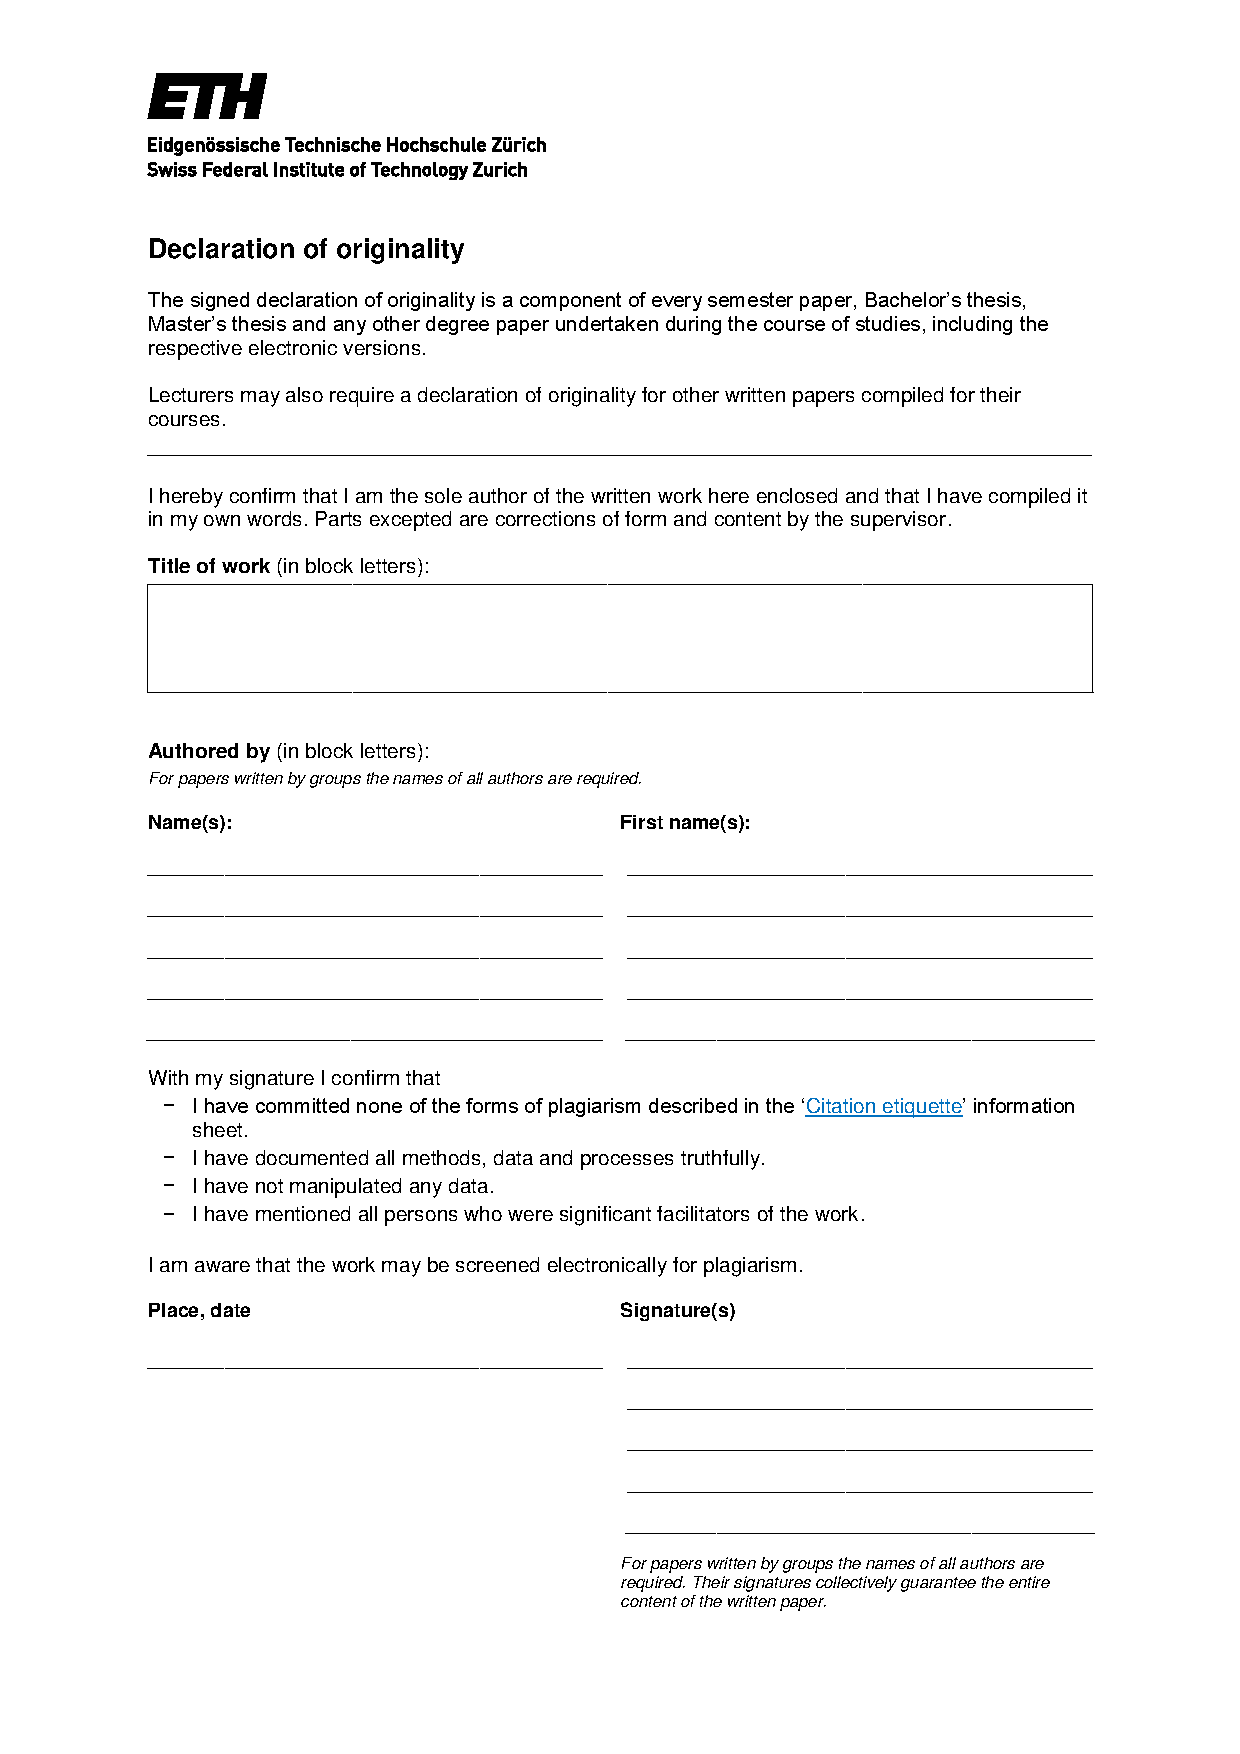
\includepdf[pages=-]{declaration-originality.pdf}

%-------------------------------------------------------------------------------
%  ABSTRACT PAGE
%-------------------------------------------------------------------------------

\begin{abstract}
\addchaptertocentry{\abstractname} % Add the abstract to the table of contents
Brief description of the thesis. Capture readers' interest. Mention/summarize everything that was done in the thesis.
\end{abstract}

%-------------------------------------------------------------------------------
%  ACKNOWLEDGEMENTS
%-------------------------------------------------------------------------------

\begin{acknowledgements}
\addchaptertocentry{\acknowledgementname} % Add the acknowledgements to the table of contents
\begin{itemize}
\itemsep0em
  \item Supervisors
  \item Professor
  \item Vasilis
  \item Joao
  \item family
  \item wg
  \item gionata
  \item Octave
  \item FullSWOF\_2D
  \item Inkscape
\end{itemize}
\end{acknowledgements}


%-------------------------------------------------------------------------------ABBREVIATIONS
%-------------------------------------------------------------------------------

\begin{abbreviations}{ll} % Include a list of abbreviations (a table of two columns)

\textbf{EP}   & \textbf{E}xpectation \textbf{P}ropagation\\
\textbf{FV}   & \textbf{F}inite \textbf{V}olume\\
\textbf{FVM}  & \textbf{F}inite \textbf{V}olume \textbf{M}ethod\\
\textbf{GCI}  & \textbf{G}rid \textbf{C}onvergence \textbf{I}ndex\\
\textbf{GC}   & \textbf{G}aussian \textbf{P}rocess\\
\textbf{IQR}  & \textbf{I}nter\textbf{Q}uartile \textbf{R}ange\\
\textbf{ML}   & \textbf{M}achine \textbf{L}earning\\
\textbf{MAE}  & \textbf{M}aximum \textbf{A}bsolute \textbf{E}rror\\
\textbf{RMSE} & \textbf{R}oot \textbf{M}ean \textbf{S}quared \textbf{E}rror\\

\end{abbreviations}


%-------------------------------------------------------------------------------
%	SYMBOLS
%-------------------------------------------------------------------------------

\begin{symbols}{lll} % Include a list of Symbols (a three column table)

$dx$      & Grid spacing in x-direction    & \si{\m} \\
$dy$      & Grid spacing in x-direction    & \si{\m} \\
$Lx$      & Domain length in x-direction   & \si{\m} \\
$Ly$      & Domain length in y-direction   & \si{\m} \\
$Nx$      & Number of cells in x-direction & 1 \\
$Ny$      & Number of cells in y-direction & 1 \\
$Q$       & Discharge                      & \si{\cubic\m\per\s} \\
$t_{max}$ & Simulation duration            & \si{\s} \\
%Symbol & Name & Unit \\

%\addlinespace % Gap to separate the Roman symbols from the Greek

\end{symbols}


%-------------------------------------------------------------------------------
%  TABLE OF CONTENTS
%-------------------------------------------------------------------------------

\tableofcontents
\seb{is that ok index up to third level? or better just second? should third level be numbered and indented as well?}


%-------------------------------------------------------------------------------
%  THESIS BODY
%-------------------------------------------------------------------------------

\mainmatter % Begin numeric (1,2,3...) page numbering

\pagestyle{thesis} % Return the page headers back to the "thesis" style

% Include the chapters of the thesis as separate files from the Chapters folder
% Uncomment the lines as you write the chapters

\chapter{Introduction}
\label{chp:introduction}
%----------------------------------------------------------------------------------------

% Define some commands to keep the formatting separated from the content 
\newcommand{\keyword}[1]{\textbf{#1}}
\newcommand{\tabhead}[1]{\textbf{#1}}
\newcommand{\code}[1]{\texttt{#1}}
\newcommand{\file}[1]{\texttt{\bfseries#1}}
\newcommand{\option}[1]{\texttt{\itshape#1}}

%----------------------------------------------------------------------------------------



Flooding and inundation have dramatically increased in the last years due to climate change.
The frequency, as well as the magnitude of extreme rain events, leading to major inundations, have grown, making our capability to predict occurrence and effects more unreliable.
To limit risks and damage, novel control, mitigation and warning measures are needed.
Design and implementation of these need preliminary study of the situation based on data and information.
Unfortunately, these are often not available, or not in the amount required for carrying out preliminary studies.

Nowadays simulation offers a valid and very powerful tool for dealing with this problem.
Hydrological numerical models of catchments can be built, where depending on the degree of detail required different processes are implemented: infiltration, evaporation, erosion, etc.
Depending on the degree of detail chosen more or less accurate models can be achieved.
These models are mainly based on topographical data of the catchment in question, which are then refined by assigning friction coefficients values, infiltration capacity values, hydraulic conductivity values, porosity values to the different zones of the catchment.
Such models need to be calibrated.
This means that by using optimization algorithms the parameters of the model are varied within certain ranges in order to reproduce at best a recorded output (e.g. river outlet hydrograph) generated from "known" initial conditions (e.g. initial soil saturation) and inputs (e.g. the recorded hyetograph).
Once the model is calibrated it can be used to generate new data, from which new information about the given system can be learned and from which other conditions and new situations can be tested.

The main drawback of simulation lays in its very high computational burden.
For calibration alone several runs of the model are required.
Every simulation can last from some minutes up to several hours, depending on the complexity of the model, the type of computer where the simulations are run, the duration of the event simulated, the resolution used for the model, etc.
Once the model is calibrated several more runs are necessary in order to generate the desired dataset.
The number of runs depends on the kind of study one would like to carry out.
For uncertainty analysis for example, up to some thousands of simulations can be run, in order to study the influence that the variation of a parameter of the model (or its uncertain determination) has on the output.\\

\ldots\\



\seb{Rearrange and somehow integrate the two previous sections in order to produce a global introduction. Introduce the following section "Emulation", a brief introduction about emulation}

% ---------------------------------------------------------------------------------------------------
% ===================================================================================================
\section{Definition of goals}
% ===================================================================================================

Focus on emulation subject.

\begin{itemize}
\itemsep0em
  \item explain what is emulation
  \item use both terms \textit{surrogate model} and \textit{emulator}
  \item mention \textit{EmuMore} project
  \item give emulation examples
\end{itemize}


% ==============================================================================
\section{Emulation}
% ==============================================================================

\begin{itemize}
\itemsep0em
  \item define the goals of this thesis
  \item state the questions which should be answered withing this thesis. Try to close the loop in the conclusions chapter (cf. Thesis example Jörg)
  \item what readers should expect from the thesis
  \item mention reproducibility, open softwares
  \item include a scheme with the \emph{emulation workflow}
\end{itemize}









\chapter{Methods}
\label{chp:methods}
% ---------------------------------------------------------------------------------------------------

% ===================================================================================================
\section{Simulation in hydrology}
% ===================================================================================================


% ---------------------------------------------------------------------------------------------------
\subsection{FullSWOF\_2D-v1.07.00}
% ---------------------------------------------------------------------------------------------------


% ---------------------------------------------------------------------------------------------------
\subsection{Development of \textit{FullSWOF\_2D} interaction tools}
% ---------------------------------------------------------------------------------------------------

\begin{itemize}
\itemsep0em
  \item explain the work done
  \item list the functions developed and their function
  \item mention \textit{fswof2d} repository
  \item explain how to install the package?? \noteseb{does this make sense here?? should go in the README}
\end{itemize}

As already mentioned in section \colseb{mention which section} \textit{FullSWOF\_2D-v1.07.00} was chosen as \emph{overland flow simulator} in order to generate the required datasets.
\textit{FullSWOF\_2D} needs at least three input files in order to run simulations:

\begin{itemize}
\itemsep0em
  \item \textit{topography}: a text file specifying the topography of the domain
  \item \textit{parameters}: a text file specifying the values set for the simulation parameters
  \item \textit{huv\_init}: a text file defining the initial conditions of the problem (initial water height and initial water velocity at every point of the grid)
\end{itemize}

In order to generate these files, interaction functions were developed with the open source tool \textit{Octave 4.2.1} \autocite{octave_community_gnu_2018}.
The interaction functions were grouped into the Octave package \textit{fswof2d} available at \url{https://bitbucket.org/binello7/fswof2d}.\\

The package includes the following functions, all of which are distributed under \textit {GPLv3} license \autocite{smith_quick_2014}.

\begin{itemize}
\itemsep0em
  \item center2node.m
  \item csec\_channel2lvlsym.m
  \item dataconvert.m
  \item extrude\_csec.m
  \item huv2file.m
  \item matplotlib\_cm.m
  \item node2center.m
  \item params2file.m
  \item read\_params.m
  \item topo2file.m
\end{itemize}

% ---------------------------------------------------------------------------------------------------
\subsection*{center2node.m}
% ---------------------------------------------------------------------------------------------------
\textit{function x = center2node (cx, x0)}\\


% ---------------------------------------------------------------------------------------------------
\subsection*{node2center.m}
% ---------------------------------------------------------------------------------------------------
\textit{function cx = node2center (x)}\\

\textit{FullSWOF\_2D} uses a regular uniform grid in order to solve the \emph{shallow water equation} with the finite volume method (FVM).
The equations are solved at the center of every cell.
After creating the vector defining the grid nodes, one can use the \textit{center2node} function to compute the centers of the grid cells.
This is particularly useful because the $(x,y)$ coordinates saved to the \textit{topography} file have to be the coordinates of the cell centers.
A short usage example would be:

\begin{lstlisting}
  # define the domain length in x-direction
  Lx = 100;
  # define the number of nodes
  Nx = 200;
  # create nodes of the regular grid in x-direction
  xn = linspace (0, Lx, Nx);
  # create vector of cell centers
  xc = node2cdenter (xn);
\end{lstlisting}



% ===================================================================================================
\section{Emulation}
% ===================================================================================================


% ---------------------------------------------------------------------------------------------------
\subsection{Regression and interpolation methods}
% ---------------------------------------------------------------------------------------------------

\begin{itemize}
\itemsep0em
  \item explain the work done on regression and interpolation
  \item explain their relation with emulation
  \item explian extrapolation, when it can be done and how reliable it can be
\end{itemize}



\chapter{Case studies}
\label{chp:case_studies}
%-------------------------------------------------------------------------------

\noindent{\LARGE\textbf{Case study 1}}
%===============================================================================
\section{A mechanistic emulator: fitting the \emph{weir equation}}
%===============================================================================

%:::::::::::::::::::::::::::::::::::::::::::::::::::::::::::::::::::::::::::::::
%  * present it as a didactic example
%  * use it to compare GP (prior knowledge) with e.g. deep neural networks: how many points can we have?
%  * mention grid convergence study (results go in the Appendix)
%  * mention problem with FullSWOF boundary conditions
%  * define well results and methodology
%  * such an emulator can be improved -> modified to compute slope in order to have a given mu value
%  * state all of the goals of the CS: learn weir eq. from simulation, apply curve fitting, get a feeling for simulation accuracy
%:::::::::::::::::::::::::::::::::::::::::::::::::::::::::::::::::::::::::::::::

As a first case study to apply the acquired knowledge, it was decided to build an utterly mechanistic emulator.
The main goal of this case study is to try to fit the \emph{weir equation} to simulated data instead of to experimental data.
Here we basically rediscover the way science has always been done: by observing, measuring and trying to find mathematical relationships.
The biggest difference is the fact that the experimental set-up is completely computer built.\\

The \emph{weir equation} is a partially theoretical equation that provides an estimate of the discharge $Q$ over a weir as a function of the water depth above the weir itself ($h_w$).
The equation can be derived from the Bernoulli equation under certain assumptions \autocite{bos_discharge_1989} and can be found under many different forms.
The form used here is the one proposed by \emph{Francis} \autocite{walcott_weir_1907}:

\begin{equation}\label{eq:weir_eq}
  Q = \textcolor{red}{C} \cdot L \cdot h_w^{\textcolor{red}{a}}\, , \quad \mbox{usu. } \textcolor{red}{a = 3/2}
\end{equation}

\noindent Where the empirical coefficient $C$ corrects for the assumption of absence of viscous effects and uniform velocity distribution. $L$ is the length of the weir (perpendicular to the channel) and $h_w$ is the water height above the weir.

In addition to the parametric model (weir equation) two non-parametric local techniques, namely \emph{linear interpolation} and \emph{cubic spline interpolation}, were used to intrapolate between the simulated data points.\\


%-------------------------------------------------------------------------------
\subsection{Brief experiment description}\label{sec:cs1_brief_description}
%-------------------------------------------------------------------------------

\seb{explain the experiment very generally. Put the section title or leave it with no section title with the upper part?}
 
For this experiment simulations were run in a flat rectangular channel.
A weir with a trapezoidal cross section is located at the channel half-length.
As initial condition the upstream side of the weir was filled with water up to the weir crest.
At the domain top boundary a constant inflow discharge was set, while at the bottom boundary water could freely outflow.
As the simulation runs, the inflow water flows down the channel, overflows the weir and leaves the domain through the lower boundary.
After some time the simulation reaches the \emph{steady-state} conditions: inflow, discharge over the weir and outflow have the same magnitude and the water height above the weir has stabilized.
At this point the value $h_w$ was extracted and was coupled with the discharge value $Q$ generating it.
\num{25} experiments were conducted with $Q$ linearly spaced in the range \SIrange{0.1}{10}{\cubic\meter\per\second}.
All simulated pairs $(Q, h_w)$ constitute an observational \emph{predictor-response} set to which the weir equation was fitted.
 \seb{give e.g. in Appendix the discharge values used? Probably not, I gave the code with linspace to generate the different discharges}\\

In order to ensure the convergence of the simulator solution, and therefore the quality of the experimental results, a \emph{grid convergence study} was performed prior to the experiment.
For this, the simulation with the highest discharge was repeated with successive grid refinements
The value of the variable of interest, water height, was then compared between the different simulations to find at which grid resolution the solution stabilizes.


%-------------------------------------------------------------------------------
\subsection{Material and methods}
%-------------------------------------------------------------------------------
%...............................................................................
\subsubsection{Generating the topography}
%...............................................................................
The topography used for running the simulations was generated in \textit{Octave} \seb{write "Octave", "FullSWOF", ... in italics?} and represents a flat channel of \SI{40}{\meter} length with a weir placed at its midpoint, at \SI{20}{\meter} distance from the top boundary.
The channel cross section is a rectangle of \SI{4}{\meter} width and the weir has a trapezoidal shape.
Fig.~\ref{fig:weir_scheme} shows the geometry of the channel.
The weir has a crest width of \SI{2}{\meter} and therefore belongs to the \emph{broad-crested} class. The $C$ coefficient for broad-crested weirs with vertical walls and \SI{2}{\meter} crest width varies between \num{1.36} and \num{1.53}, depending on the water height $h_w$ \autocite{brown_urban_2009}.
We therefore expect a value close to this for our experiment.
A 3D overview of the channel can be found in Fig.~\ref{fig:channel} in the Appendix. \seb{add a 3D plot of the channel?}

\begin{figure}[h]
  \centering
  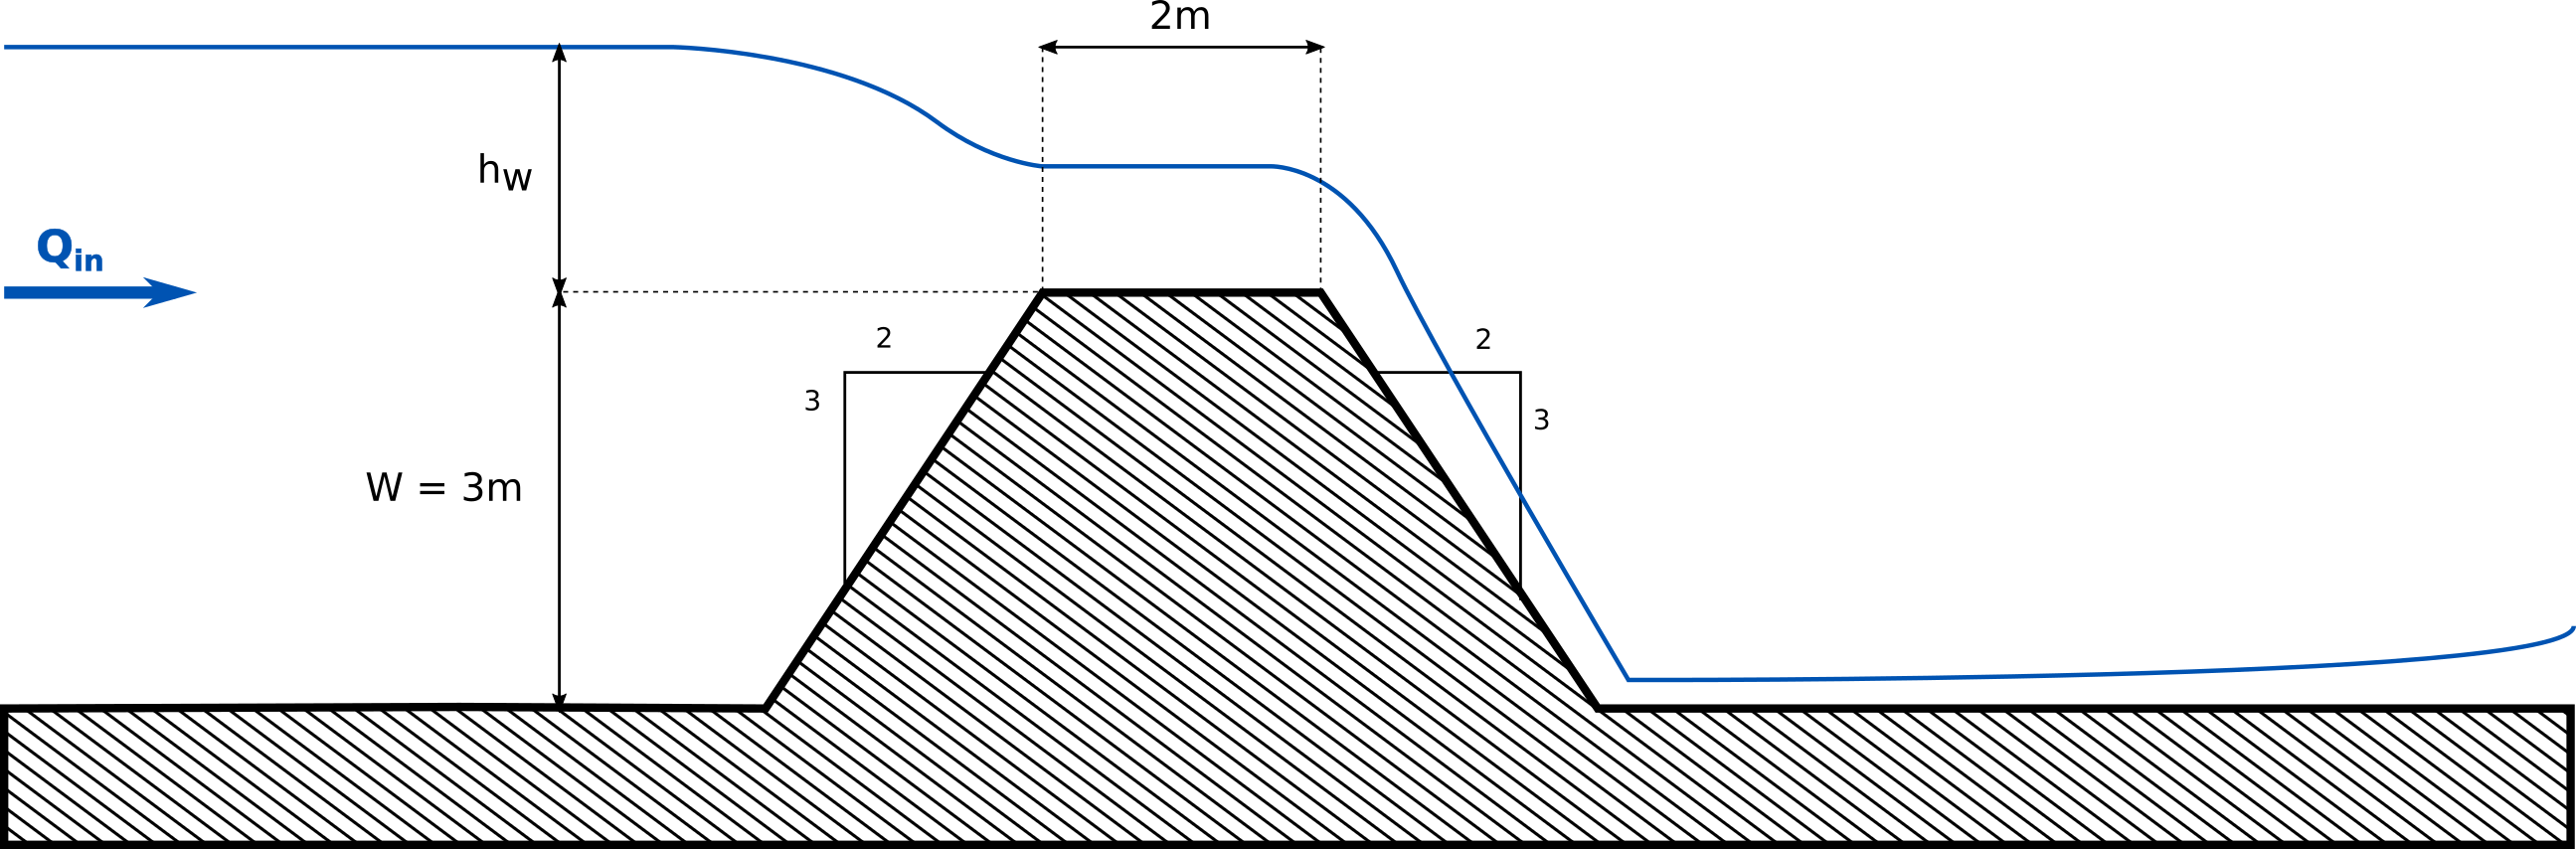
\includegraphics[width=0.8\textwidth]{Figures/weir_scheme.png}
  \caption{Geometry of the weir used for the experiments.}
  \label{fig:weir_scheme}
\end{figure}

%...............................................................................
\subsubsection{Setting-up the simulations}
%...............................................................................
After generating the topography to be used for the experiment the simulation parameters were defined and saved to the parameters file.

The simulation was done with no rain and no infiltration.
This way, water just enters the system through the top boundary and leaves it through the bottom one.
For this a \emph{Neumann} boundary condition was chosen at the bottom, while an \emph{imposed discharge} boundary condition was set at the inflow boundary.
This boundary condition needs two values to be specified: the magnitude of the inflow and an imposed water height, which is used under supercritical flow conditions.
The \num{25} inflow discharges used were obtained with the following \emph{Octave/MATLAB} code.\\

\inputminted[
  fontsize=\footnotesize,
  firstline=4,
  lastline=5,
  numbersep=2pt,
  gobble=0,
  frame=none,
  bgcolor=light-gray,
  framesep=10mm
]{octave}{code.m}\\

\noindent Where the minus sign indicates that water steadily \emph{enters the domain}.
The imposed height was set to \SI{3}{\m}, corresponding to the weir height.

The channel topography presents no banks.
Wall boundary conditions were set for the lateral boundaries in order to produce the rectangular cross section.
The wall boundaries extend infinitely high, preventing the water from overflowing.
Simulations were run for $t_{max} = \SI{200}{\s}$ and \num{200} intermediate states were saved, giving a time resolution of the simulation output of \SI{1}{\s}.
For the channel a uniform Manning roughness coefficient of \SI{0.03}{\s\per\m\tothe{1/3}} was used.

Since infiltration was not active for the simulations, all of the parameters relative to the soil model did not have to be set.

The number of cells in x, and in y direction were defined according to the grid convergence study explained here below.

%...............................................................................
\subsubsection{Conducting the grid convergence study}
%...............................................................................
\seb{better to keep a separated section, including methods and results like done here, or split it up under "material and methods" and "results and discussion"?}

\paragraph{Introduction} Accuracy of simulation results, as well as simulation runtime, are dependent on the grid resolution chosen.
In order to find an appropriate grid resolution, a grid convergence study was performed.
Successive refinements were tested in order to find out from which grid resolution the solution stabilizes, becoming independent from the resolution used.
A criterion has to be established, in order to decide when the solution has converged to a satisfactory result.
If the Grid Convergence Index (GCI) is used, then a GCI lower than \SI{5}{\percent} for the last refinement is usually taken as a criterion \autocite{ali_grid_2009}.

\paragraph{Set-up} For the mesh study \num{7} simulations were run by varying the grid resolution ($Nx$, $Ny$) only. \seb{those are mentioned in the "list of symbols". Does this help understand what was varied?}
Topography and parameters used are those mentioned in the two preceding sections.
Squared cells were used and the inflow discharge was set to the highest discharge value of the experiment, namely \SI{10}{\cubic\meter\per\second}.
This discharge is the one generating the highest flow velocities.
If convergence under these conditions is reached, then convergence for lower discharges is also assured.
Tab.~\ref{tab:mesh_study} summarizes the simulations main characteristics.

\seb{how to indicate units in the table?}
\begin{table}[h]
  \centering
  \caption{Summary of simulations runtime, grid resolution and other related parameters for the mesh convergence study.}
  \label{tab:mesh_study}
  \begin{tabular}{crrcccccr}
    \toprule
%    \rowfont{\bfseries}
    \multirow{2}{*}{\#} & \multicolumn{1}{c}{Nx} & \multicolumn{1}{c}{Ny} & \multicolumn{1}{c}{Lx} & \multicolumn{1}{c}{Ly} & \multicolumn{1}{c}{dx} & \multicolumn{1}{c}{dy} & \multicolumn{1}{c}{Q} & \multicolumn{1}{c}{runtime} \\
       & \multicolumn{1}{c}{$/1$} & \multicolumn{1}{c}{$/1$} & \multicolumn{1}{c}{$/\si{\meter}$} & \multicolumn{1}{c}{$/\si{\m}$} & \multicolumn{1}{c}{$/\si{\m}$} & \multicolumn{1}{c}{$/\si{\m}$} & \multicolumn{1}{c}{$/\si{\cubic\m\per\s}$} & \multicolumn{1}{c}{$/\si{\minute}$} \\ 
    \midrule
    1  & 2             & 20            & 4               & 40          & 2.00        & 2.00        & 10                      & 0.00 \\
    2  & 4             & 40            & 4               & 40          & 1.00        & 1.00        & 10                      & 0.07 \\
    3  & 8             & 80            & 4               & 40          & 0.50        & 0.50        & 10                      & 0.60 \\
    4  & 20            & 200           & 4               & 40          & 0.20        & 0.20        & 10                      & 9.00 \\
    5  & 40            & 400           & 4               & 40          & 0.10        & 0.10        & 10                      & 69.60 \\
    6  & 80            & 800           & 4               & 40          & 0.05        & 0.05        & 10                      & 537.72 \\
    7  & 100           & 1000         & 4               & 40          & 0.04        & 0.04        & 10                      & 1048.40 \\
    \bottomrule
  \end{tabular}
\end{table} \seb{put runtime here? Or somehow separate it, or do not put it at all?}

\paragraph{Results} Fig.~\ref{fig:water_profiles} shows the free surface profiles of the \num{7} simulations at steady-state conditions along the channel axis.
It can be noticed that for $Ny =$ \numlist{20;40;80} the water depth is visibly higher than for further refinements, and its shape quite varying.
This means that the solution has not converged yet.
Results for $Ny =$ \numlist{400;800;1000} are very close, since the lines are almost overlapping.
$Ny =$ \num{200} shows a similar profile shape, but the height is still diverging quite a bit from the successive refinements.
To better observe the variations between the different refinements, the $h$ value convergence at the weir crest was studied.

\seb{how to indicate units in graphs / diagrams? (unit)? [unit]? /unit?}
\begin{figure}[h]
  \centering
  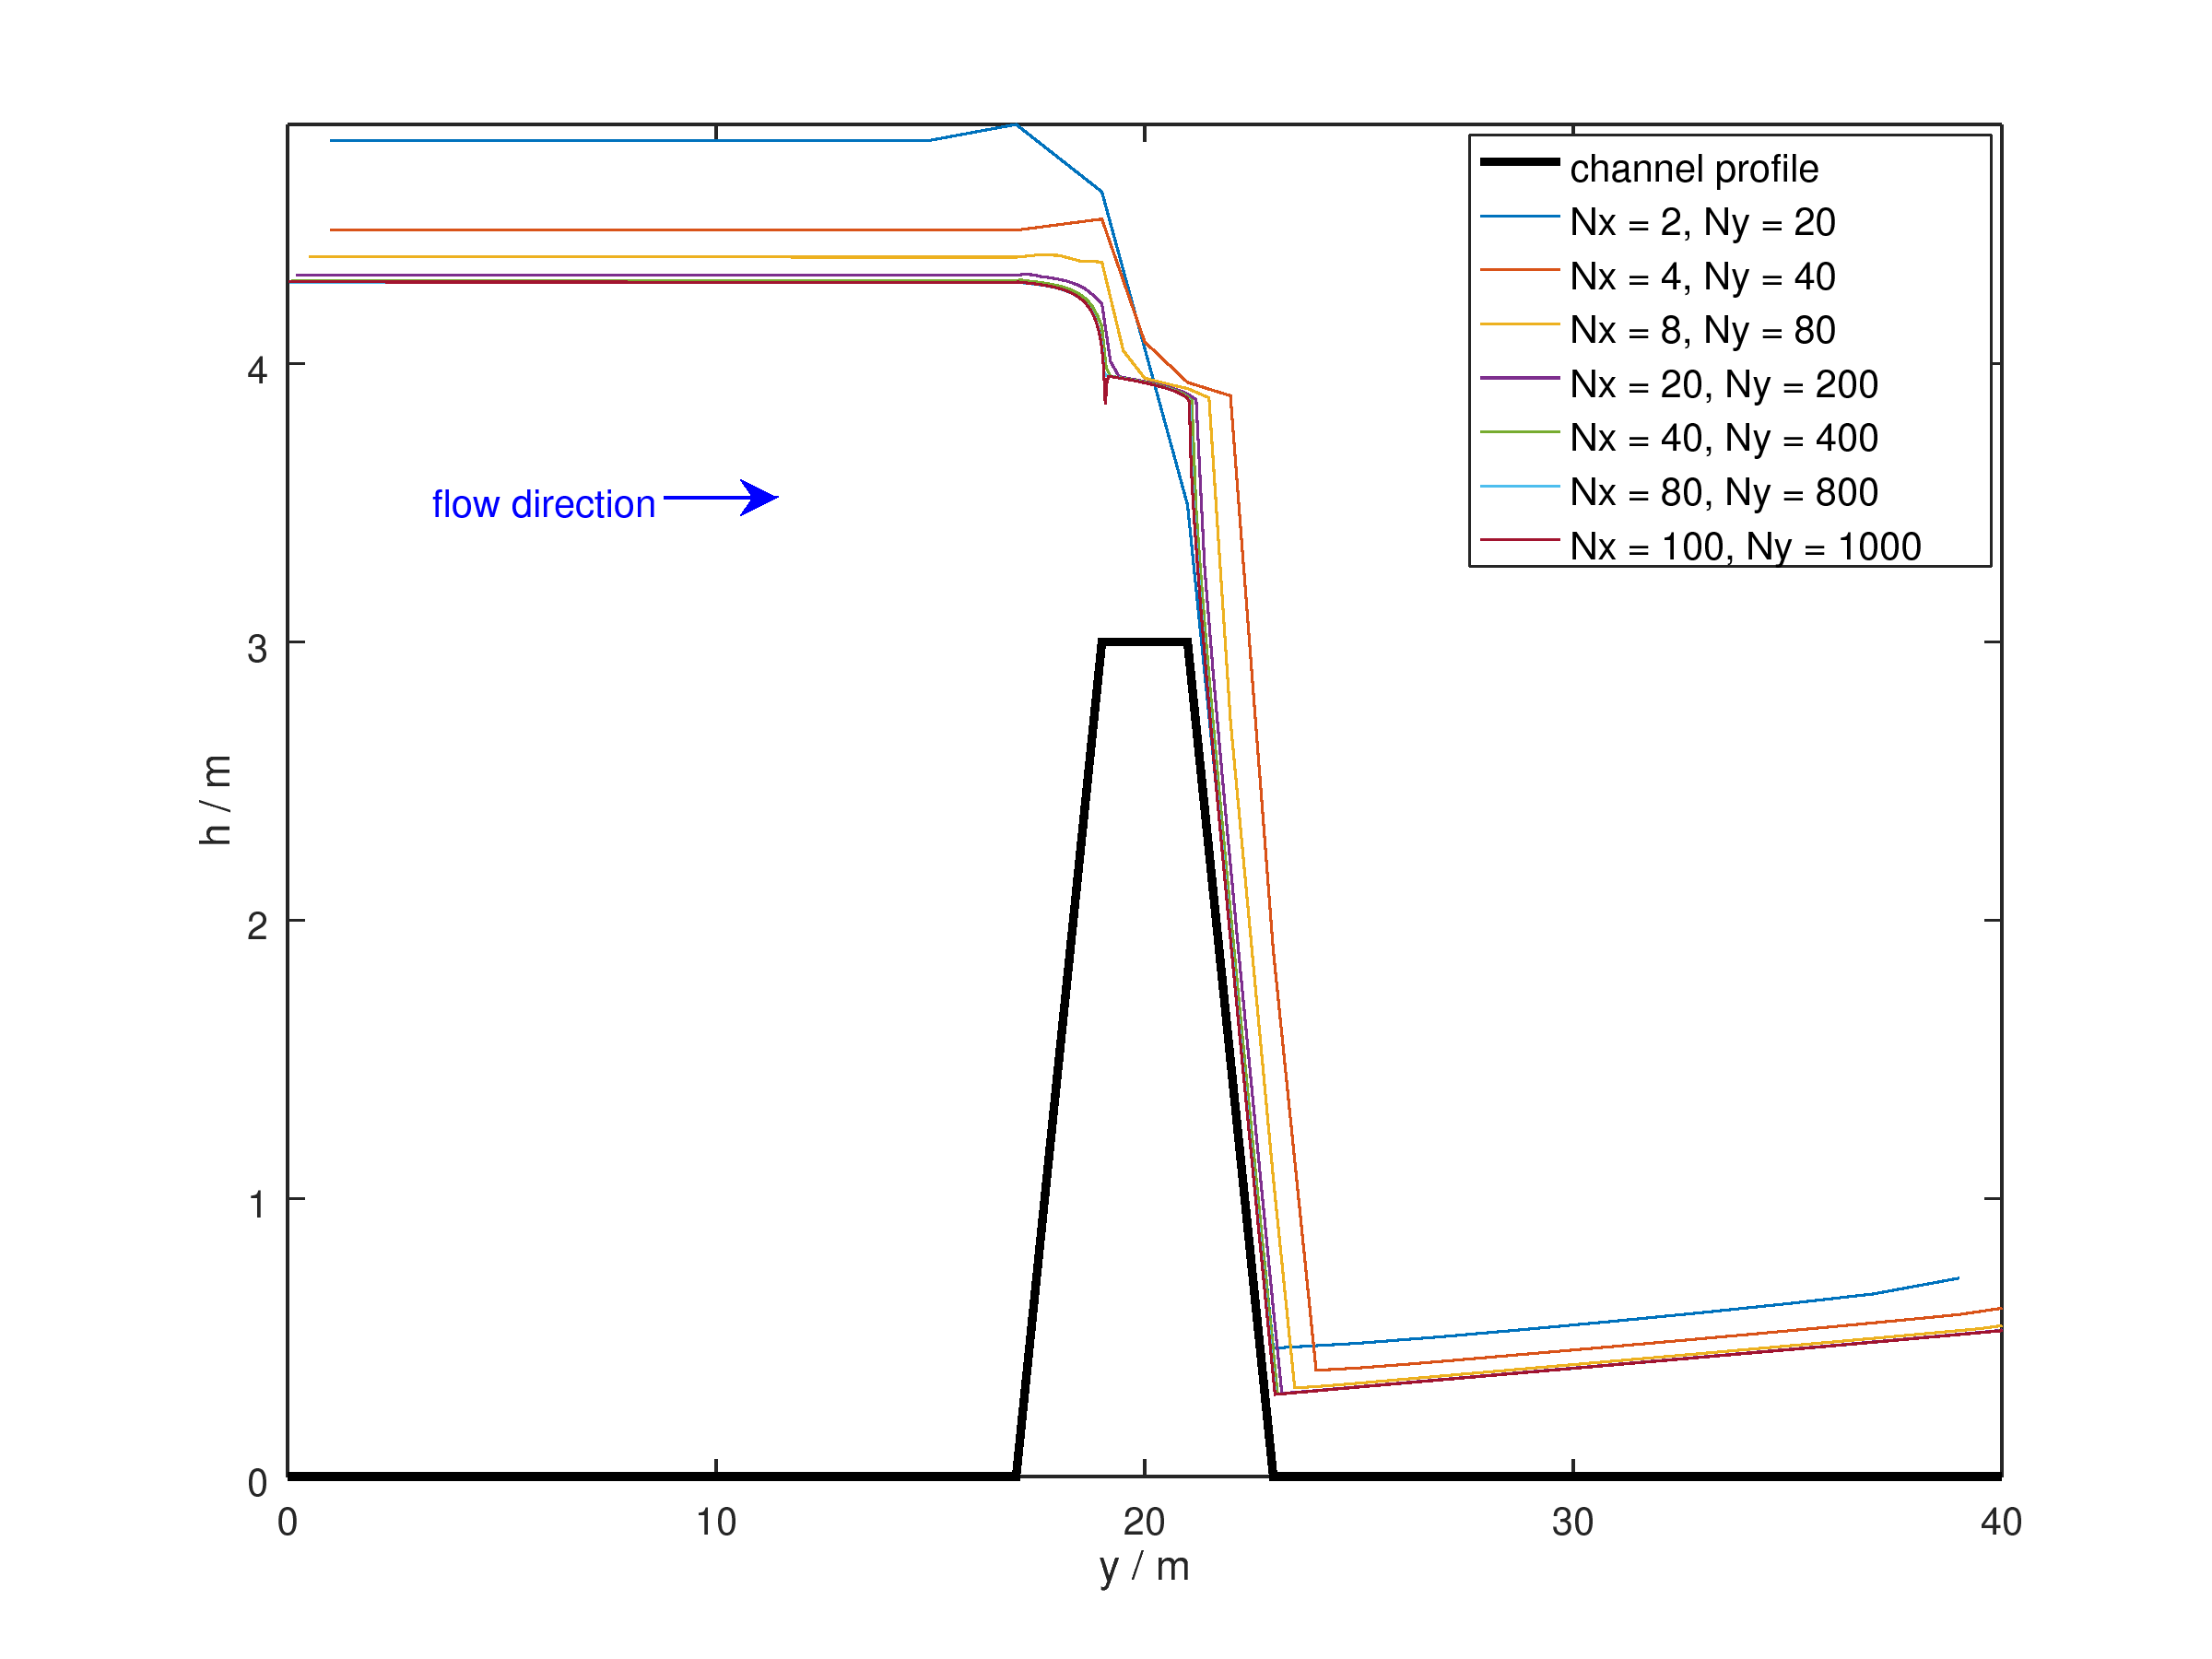
\includegraphics[width=0.7\textwidth]{Figures/water_profiles.png}
  \caption{Longitudinal free surface profiles at steady-state conditions for the \num{7} different grid resolutions.}
  \label{fig:water_profiles}
\end{figure}

In Fig.~\ref{fig:diff_center} the percent variation in the value of $h$ can be observed.
Measured absolute $h$ values at the weir center can be observed in Fig.~\ref{fig:convergence_center} in the Appendix. 
At the \nth{4} refinement the percent variation is smaller than \SI{0.01}{\percent}.
This variation is small enough to assert that the solution has satisfactory converged.
For the experiment it was therefore decided to use $(Nx, Ny) = (\num{40}, \num{400})$ corresponding to a grid resolution of \SI{0.10}{\m} in both x and y directions. The simulation runtime of $\approx \SI{1}{\hour} \SI{10}{\minute}$, required for this resolution is still quite acceptable.

\begin{figure}[h]
  \centering
  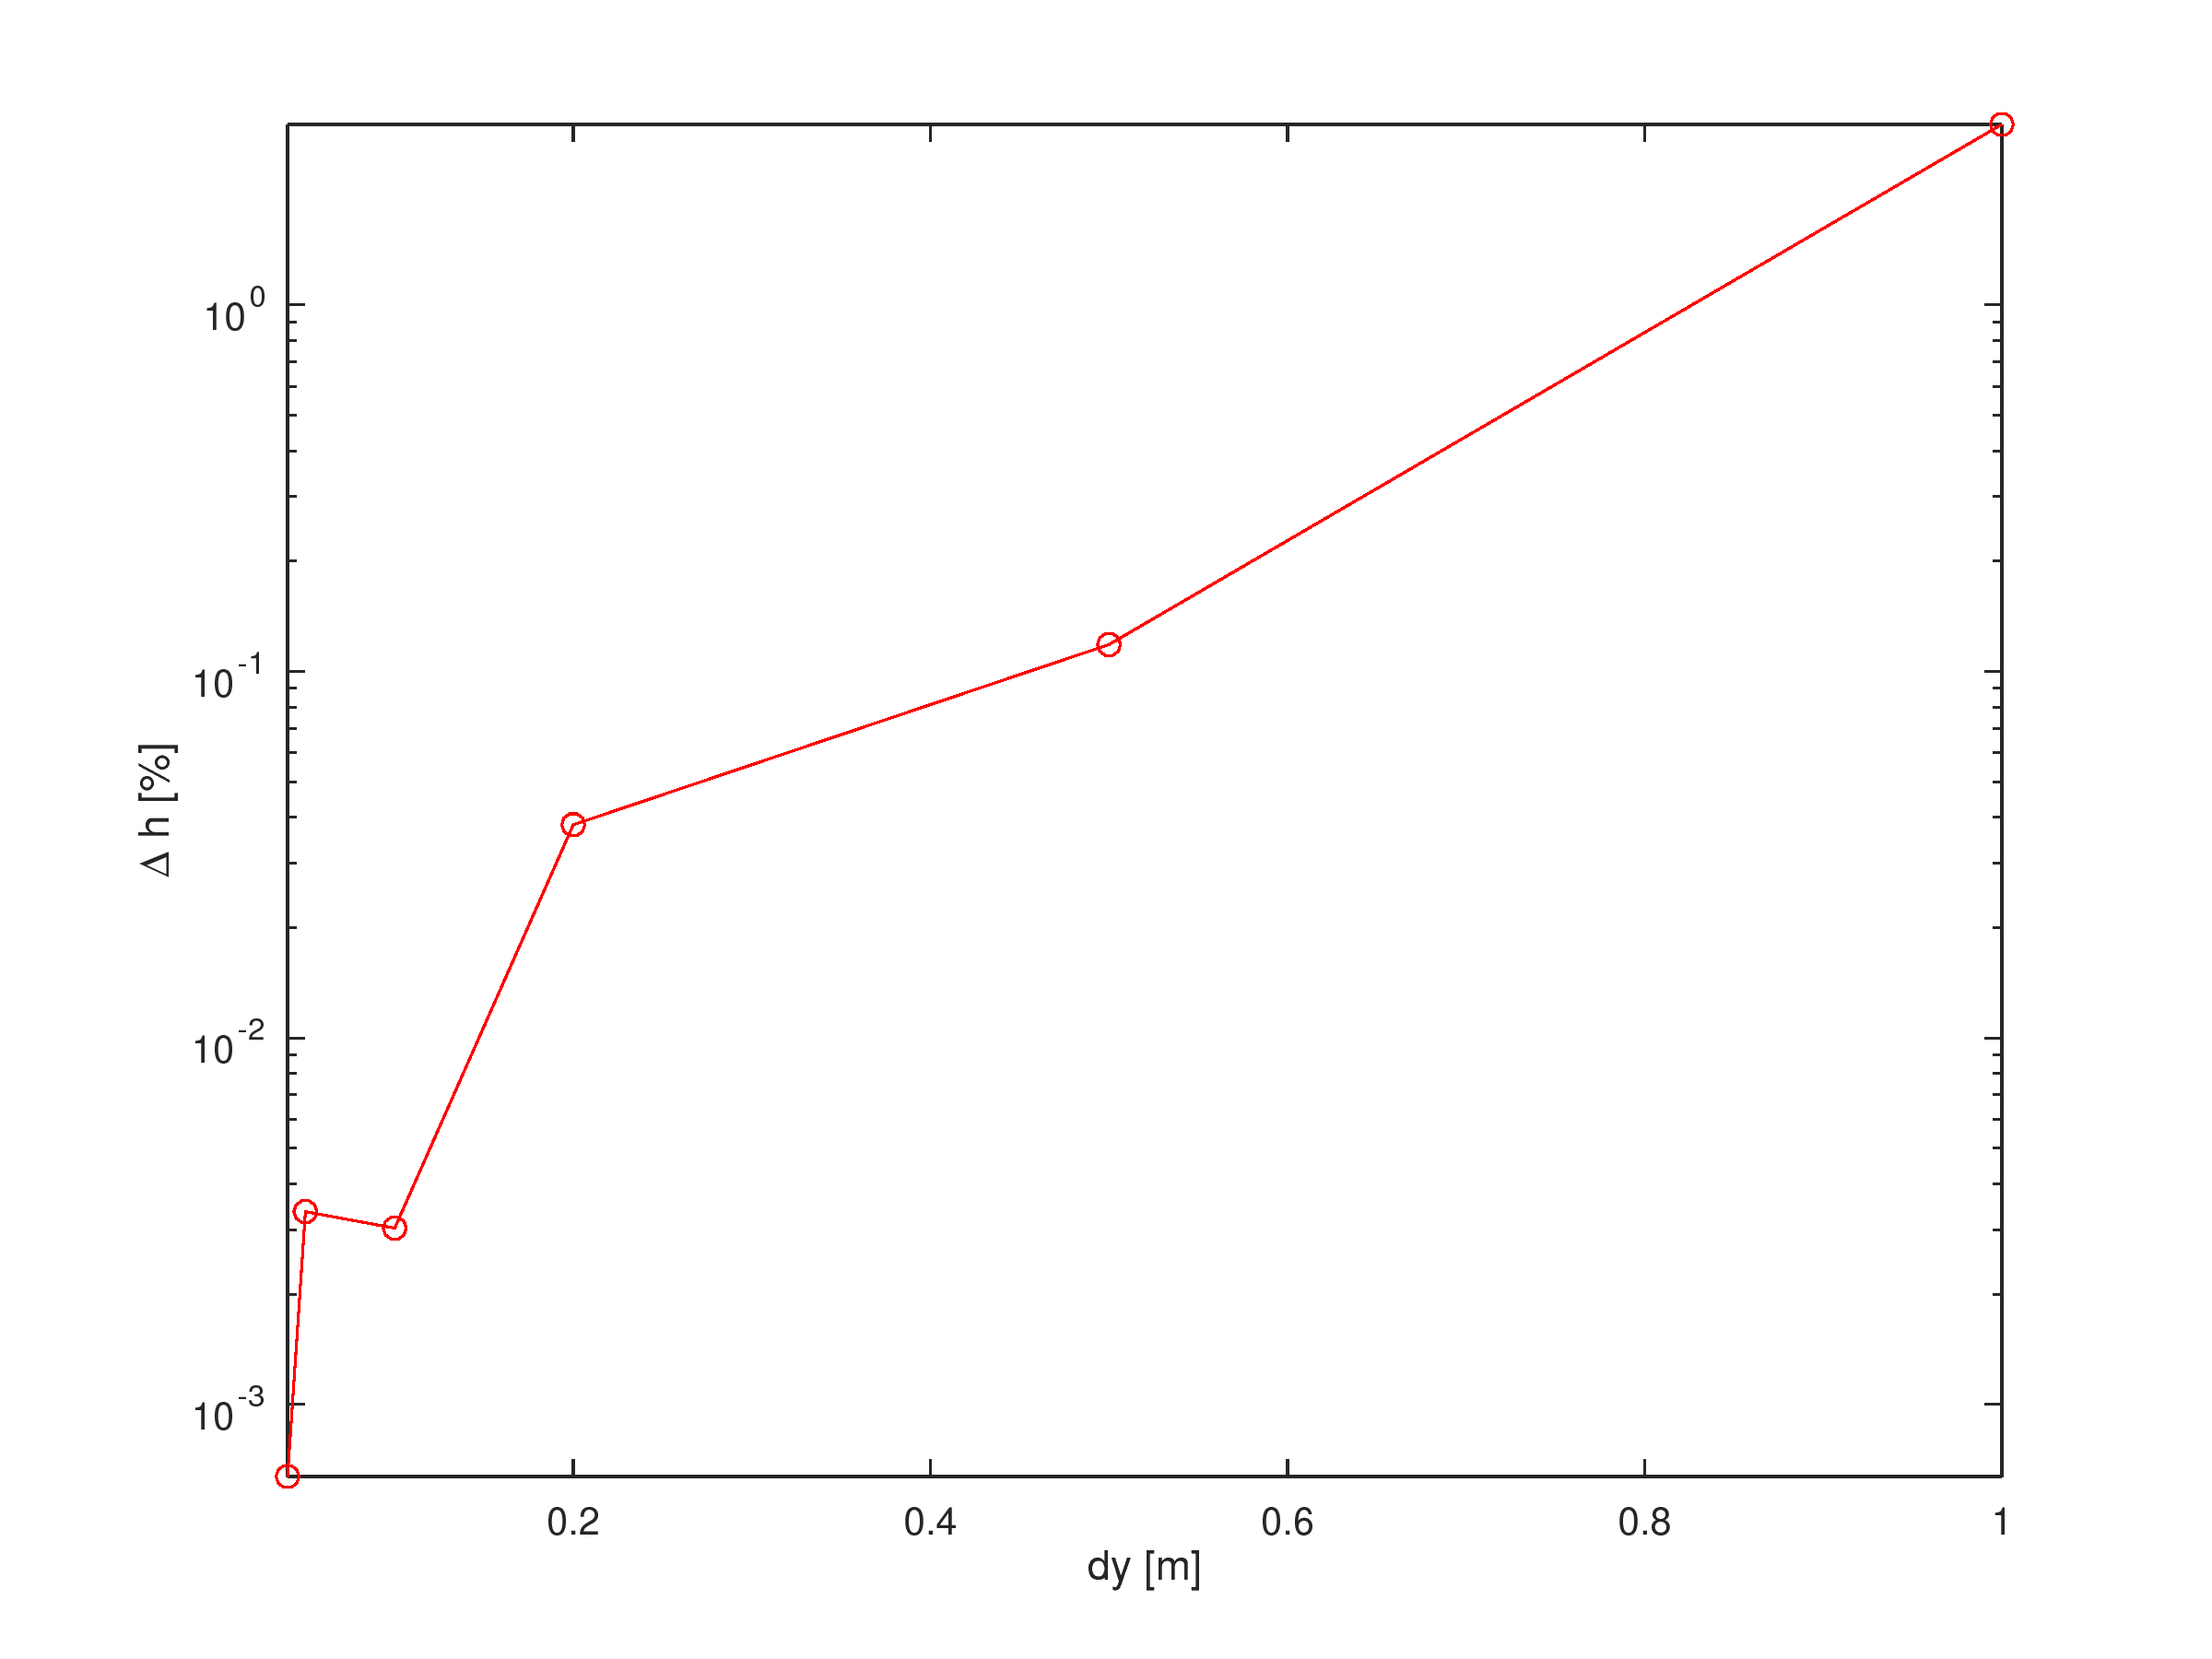
\includegraphics[width=0.7\textwidth]{Figures/diff_center.png}
  \caption{Percent variation of the measured $h$ at the weir midpoint between the given $dy$ and the previous one.}
  \label{fig:diff_center}
\end{figure}
\seb{Figure 3.3 moves to another section... is that ok??}

%...............................................................................
\subsubsection{Extracting the dataset}
%...............................................................................
The weir equation computes the discharge over the weir as a function of the water height $h_w$ under steady-state conditions.
These are reached after $\approx \SI{50}{\s}$ of simulation.
After this time, small oscillation of the water surface are still present.
To get rid of these, a time averaged free surface from $t = \SI{100}{\s}$ to $t = \SI{200}{\s}$ was computed.
Fig.~\ref{fig:free_surfaces} presents the free surface profiles of the \num{25} experiments at steady-state conditions obtained after this \emph{time smoothing out}.
The three lowest profiles correspond to the simulation runs with the three lowest inflow discharges. 
As initial condition the weir upstream side of the channel was filled with water to the weir's height.
The fact that these three profiles are lower than the initial condition indicates that something went wrong with the simulation and water was lost from the top boundary.
These simulations were discarded for the continuation of the experiment.
The height value for the remaining simulations was extracted \SI{1.2}{\m} before the weir base, to avoid observations in the acceleration zone, happening in proximity of the weir crest.
At this point a space average over the channel breadth was taken.
The procedure was repeated for all of the experiments.

\begin{figure}[h]
  \centering
  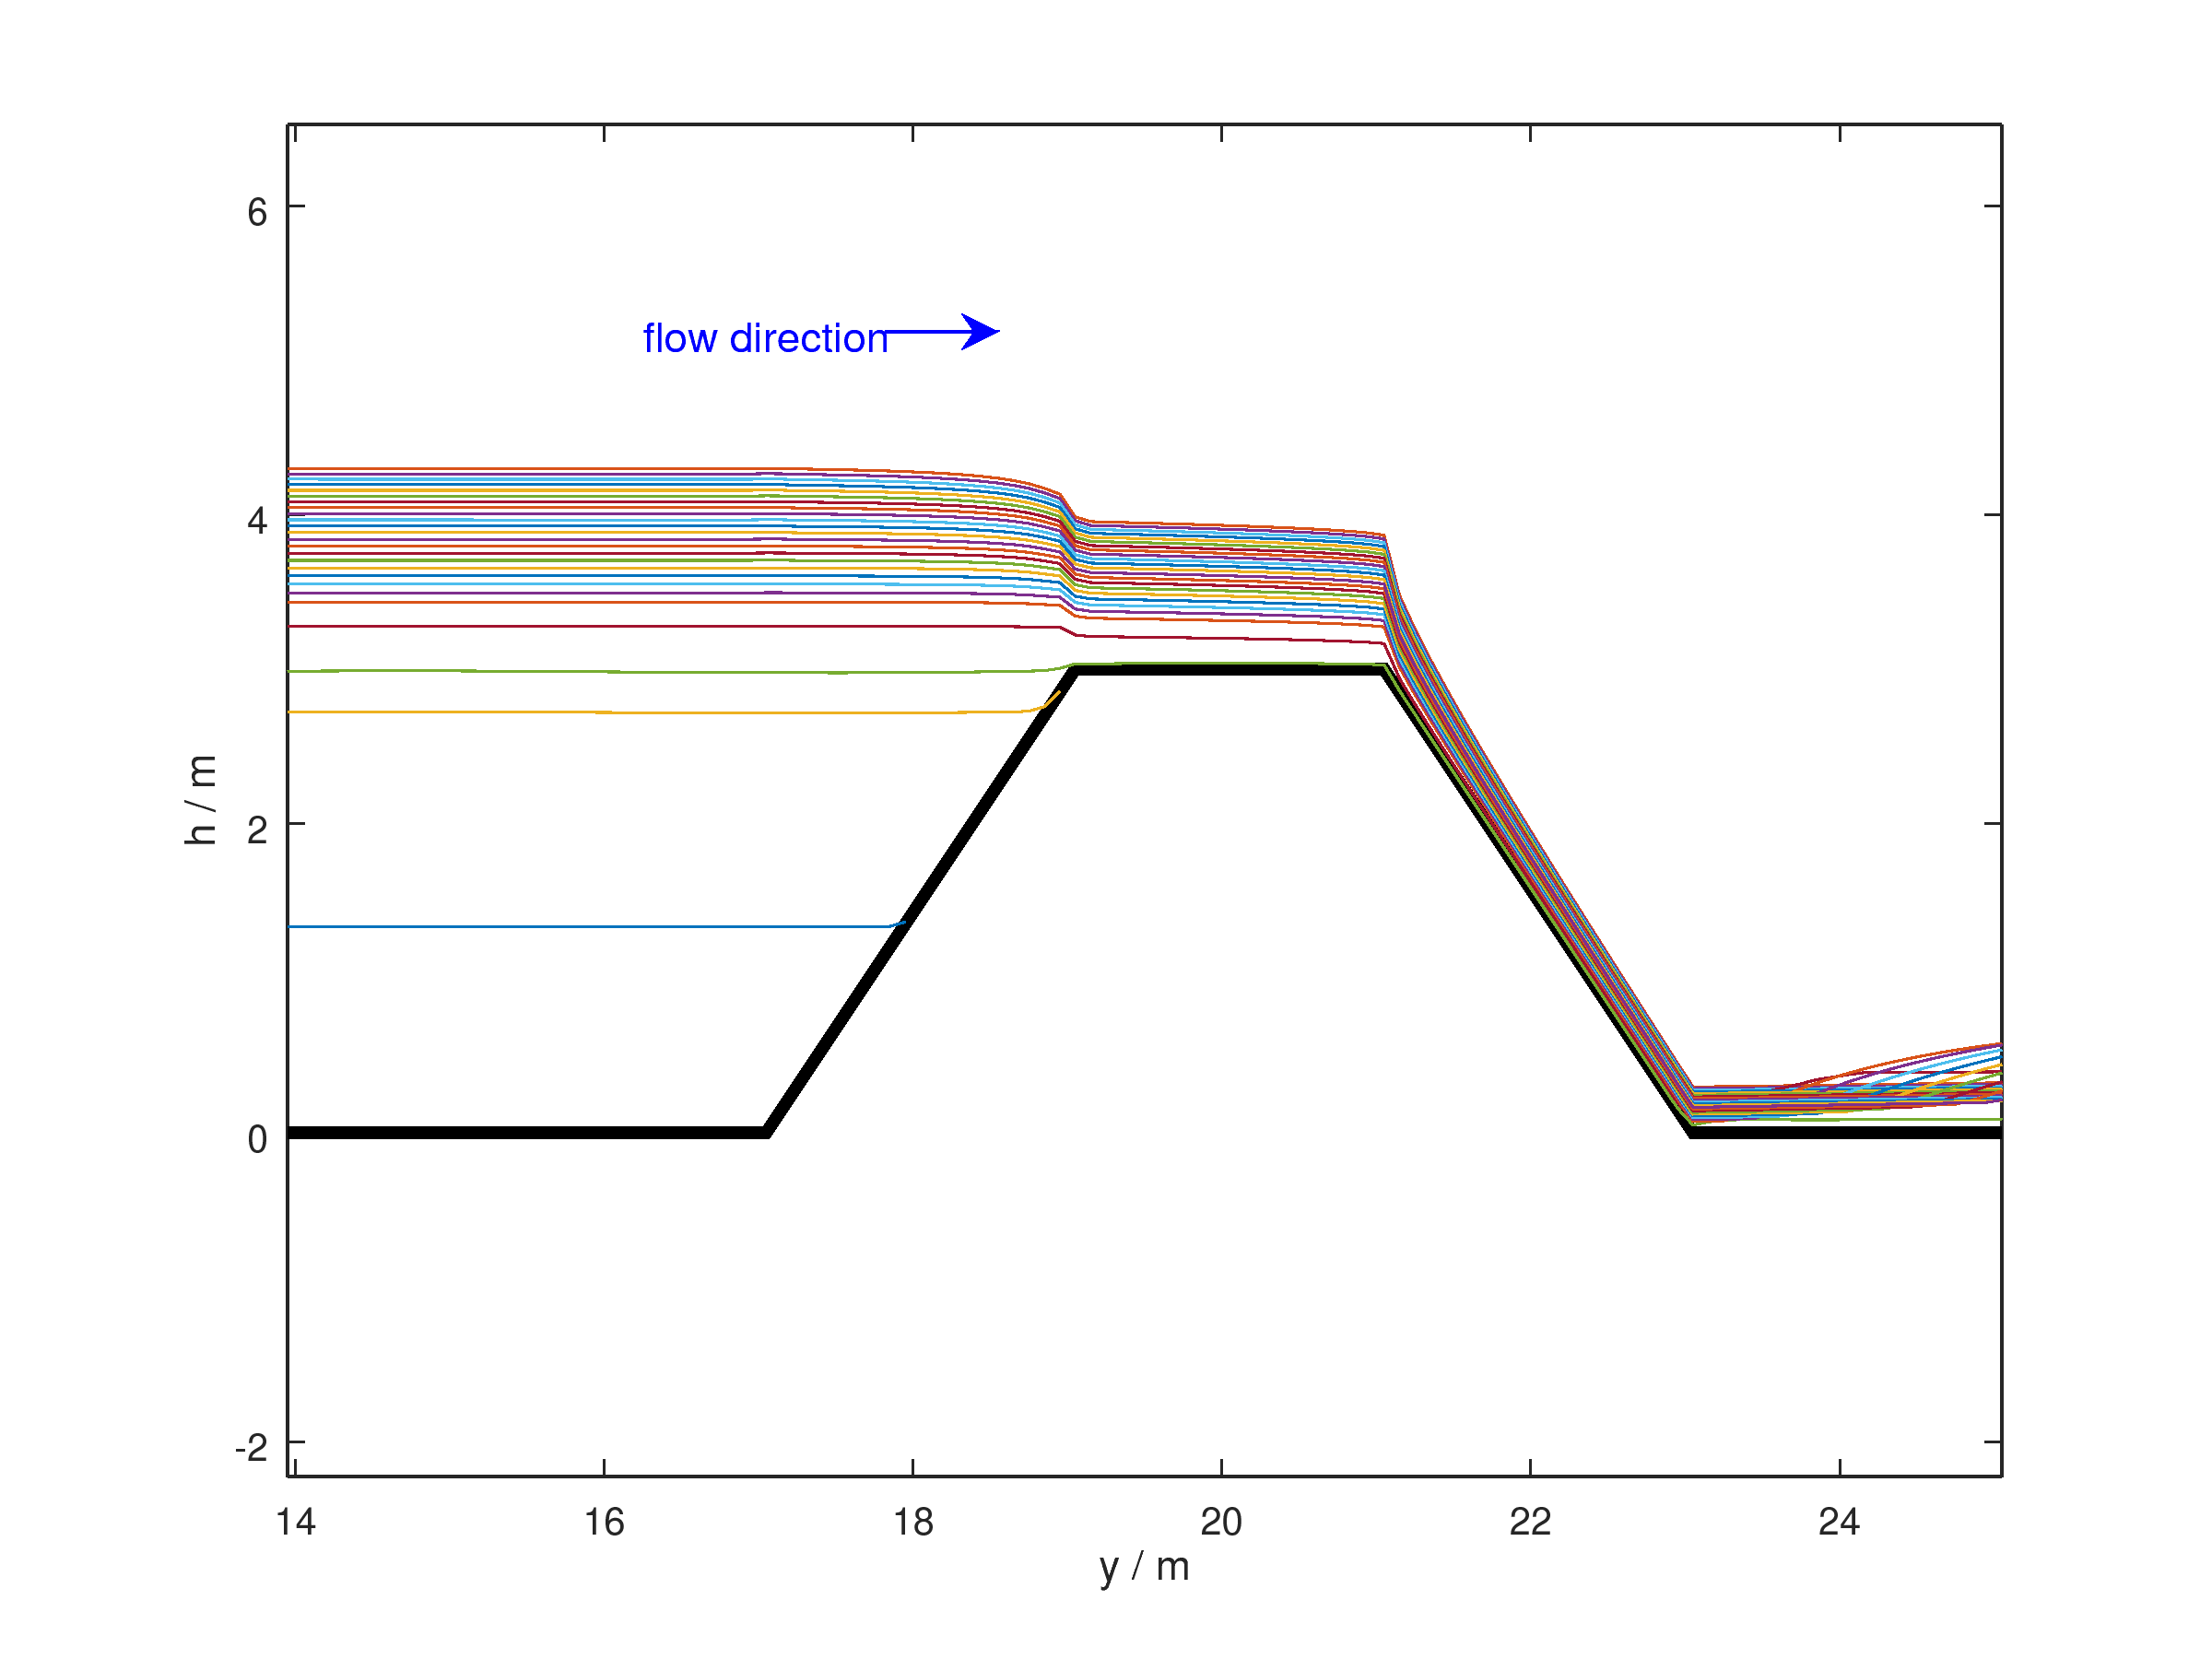
\includegraphics[width=0.7\textwidth]{Figures/free_surfaces.png}
  \caption{Free surface profiles along the channel axis for the \num{25} experiments.}
  \label{fig:free_surfaces}
\end{figure}


%...............................................................................
\subsubsection{Fitting the data}
%...............................................................................
The weir equation (Eq.~\ref{eq:weir_eq}) was fitted to the dataset previously extracted using linear regression.
The original weir equation is non-linear with respect to the parameters, it was thus linearized by taking the logarithm:

\begin{equation}
  \log(Q) = \log(C) + \log(L) + a \cdot \log(h_w)
\end{equation}

\noindent and the values of the parameters $a$ and $C$ were determined.
The performance of the fitted weir equation should be compared with that of a linear interpolation through the points and that of a cubic spline interpolation.
Therefore, the points were interpolated with both methods.


%...............................................................................
\subsubsection{Computing the error}\label{sec:compute_error}
%...............................................................................
To evaluate the performance of the three models, an increasing number of observations were removed, the models were trained on the remaining observations and it was tried to predict the ones removed.
For an amount $k$ of points removed all possible combinations were tested. The number of model evaluations follows:

\begin{equation}
  \binom{n}{k} = \frac{n!}{k!\left(n-k\right)!}
\end{equation}

\noindent Since this number grows very fast a subset of the initial dataset was used.
This can be found in Tab.~\ref{tab:dataset_error} in the Appendix.
The first and last points of the dataset were kept during all the \emph{cross-validation} experiment in order to avoid wild extrapolation at the boundaries of the predictor space.
From the remaining \num{12} points all possible combinations of \num{1} to \num{10} points were removed.
The root mean squared error (RMSE) of every combination was computed and the average RMSE for the removal of \num{1} up to \num{10} points was taken.


%-------------------------------------------------------------------------------
\subsection{Results and discussion}
%-------------------------------------------------------------------------------
% * importance of prior knowledge -> even if few points we can obtain good
%   models. Not the case without (lin. interp, spline interp.)


In Fig.~\ref{fig:simulations_results} the $(Q, h_w)$ pairs extracted from the simulations are plotted.
The gap in the lower part of the plot is due to the data that had to be discarded.
These points represent the dataset which was used to fit the weir equation and the other two models.

\begin{figure}[h]
  \centering
  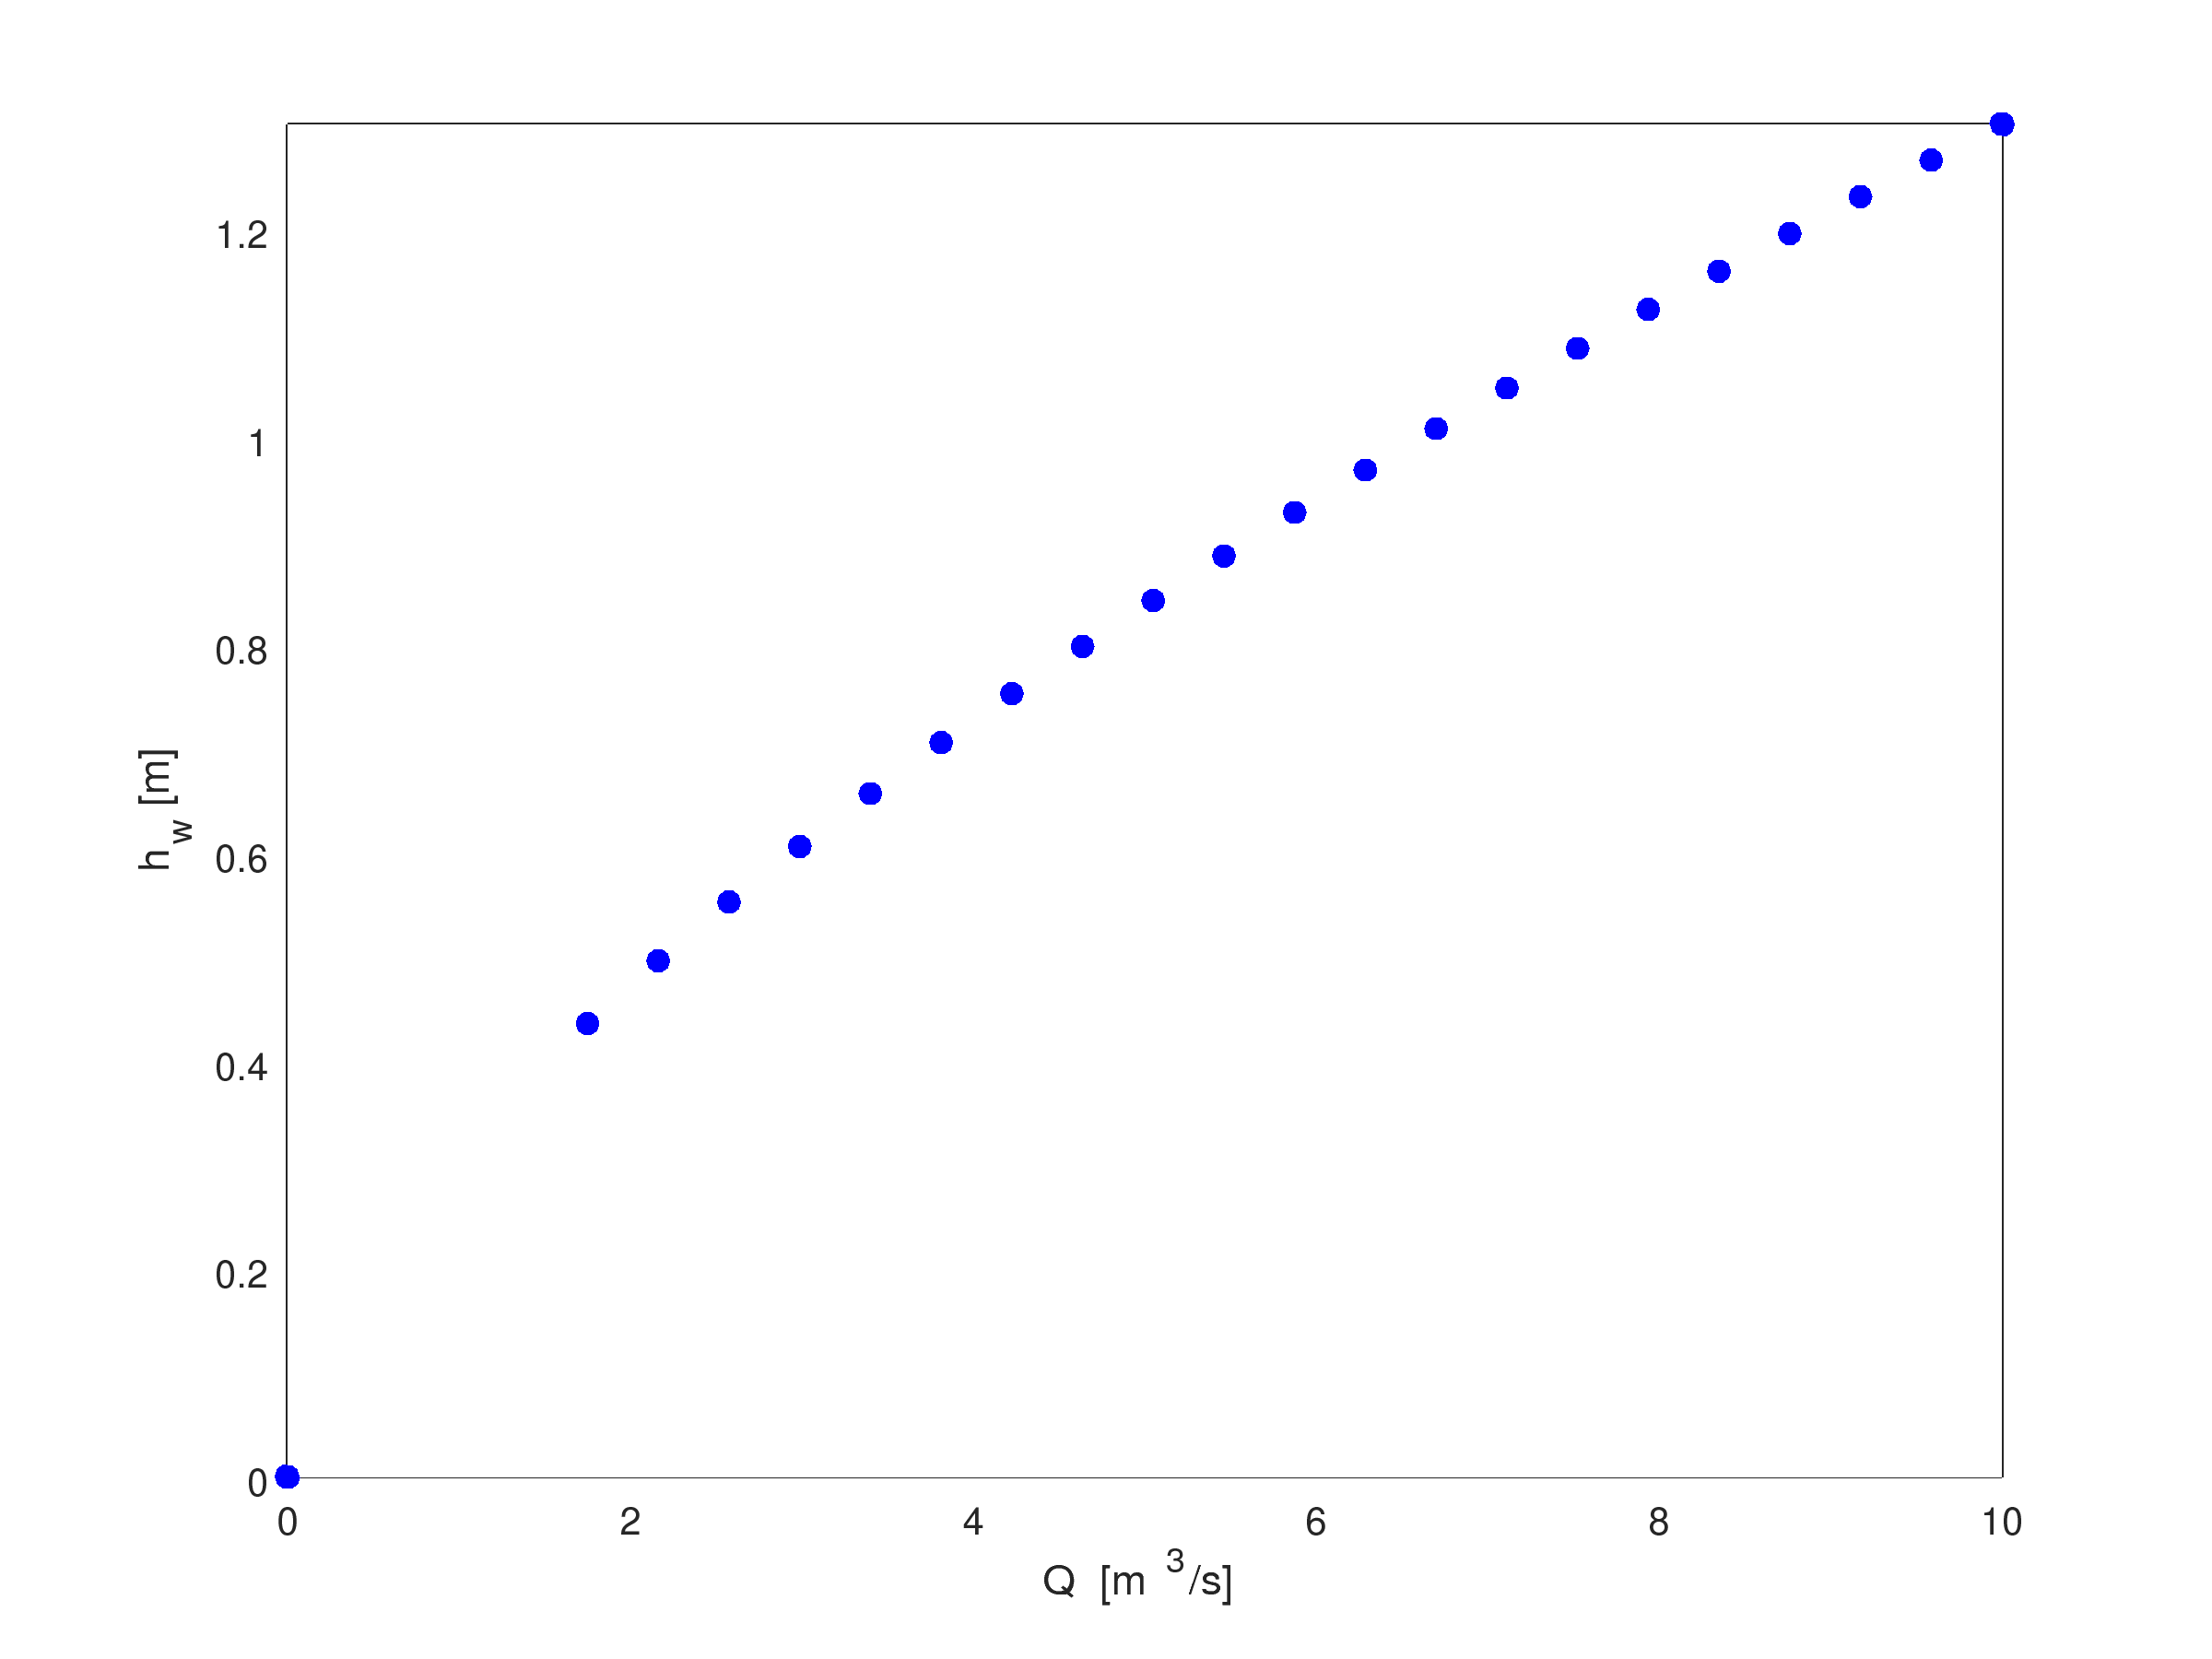
\includegraphics[width=0.7\textwidth]{Figures/simulations_results.png}
  \caption{Plot of the $(Q, h_w)$ pairs extracted from the simulations. Points corresponding to the unsuccessful simulations have already been discarded. This produces the gap visible in the left part of the plot.}
  \label{fig:simulations_results}
\end{figure}

The fit of the different models to the dataset is displayed in Fig.~\ref{fig:fitting_results}.
It can immediately be observed that the linear interpolation fails to capture the initial trend shown by the weir equation and the cubic spline interpolation.
This is due to two main reasons.
The first one is that the density of data points in this region is low---the linear interpolation simply joins the two nearest points with a segment---and on such a long distance it can diverge quite a lot from non-linear models.
Moreover, in this region the weir equation presents its maximum curvature.
This makes the linear interpolation diverge even faster.

From the second to the last point all models seem to perform good: the three lines are almost perfectly overlaying, meaning that all give very similar results.
Some divergences can be observed in proximity of data points, especially between the weir equation and the other two models: this is due to the fact that the two interpolations \emph{interpolate} the points, whereas the curve obtained for the weir equation represents the best linear fit to the points (\mintinline{octave}{polyfit (x, y, 1)}).
This minimizes the least-squares-error of the fit \autocite{eaton_gnu_2016}, which does not necessarily means interpolating through the points.

\begin{figure}[h]
  \centering
  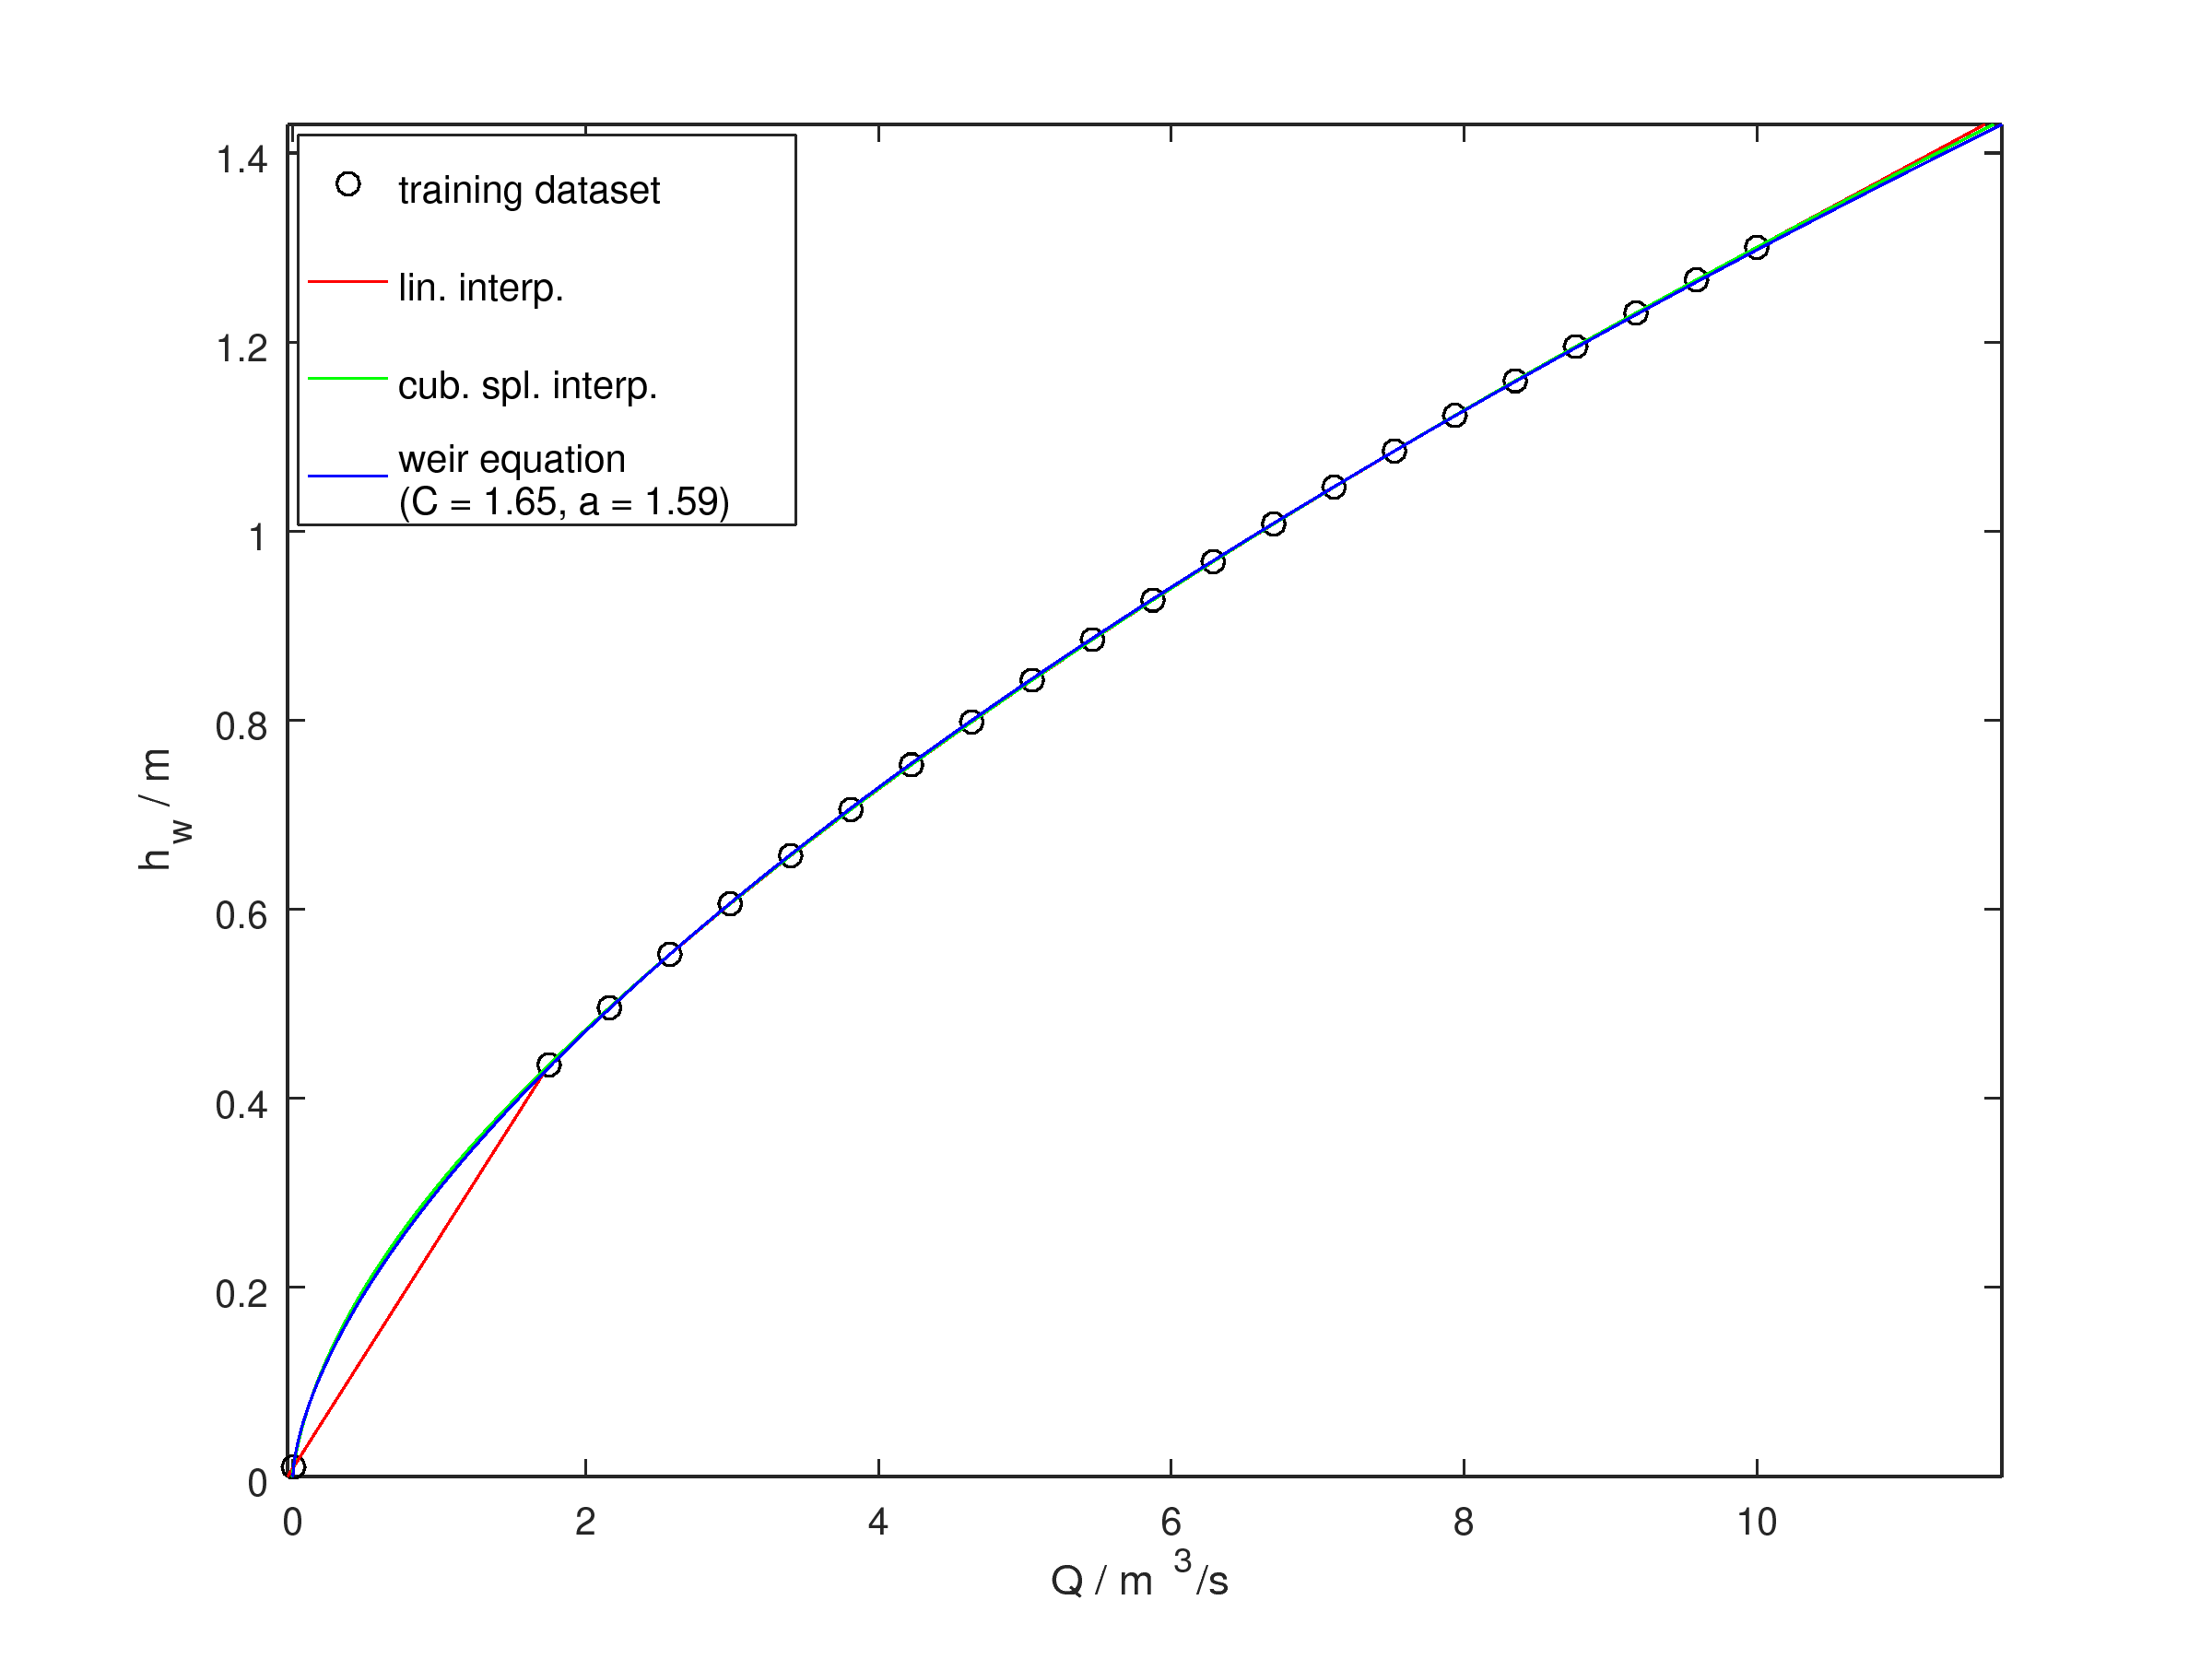
\includegraphics[width=0.7\textwidth]{Figures/fitting_results.png}
  \caption{Fit of the three models to the simulated dataset. In blue the weir equation with $C = \num{1.65}$ and $a = \num{1.59}$, in red the linear interpolation through the points and in green the cubic spline interpolation.}
  \label{fig:fitting_results}
\end{figure}

For the fitting of the weir equation the values $C = 1.65$ and $a = 1.59$ were found.
As mentioned in Sec.~\ref{sec:cs1_brief_description} for a weir of \SI{2}{\m} breadth and vertical walls $C$-values in the range $[\numrange{1.36}{1.53}]$ are expected, depending on the magnitude of $h_w$.
The value obtained for $C$ assumes that $C$ does not vary with $h_w$.
Moreover, the weir used for the experiment has a trapezoidal cross section instead of a rectangular one.
\cite{tracy_discharge_1957} investigated how the coefficient $C$ varies with different weir shapes.
For a weir with sloping walls the $C$ coefficient increases, because the head losses in comparison to one with vertical walls are lower.
The difference in the $C$ coefficient observed here can be explained by this phenomenon.\\

\begin{figure}[h]
  \centering
  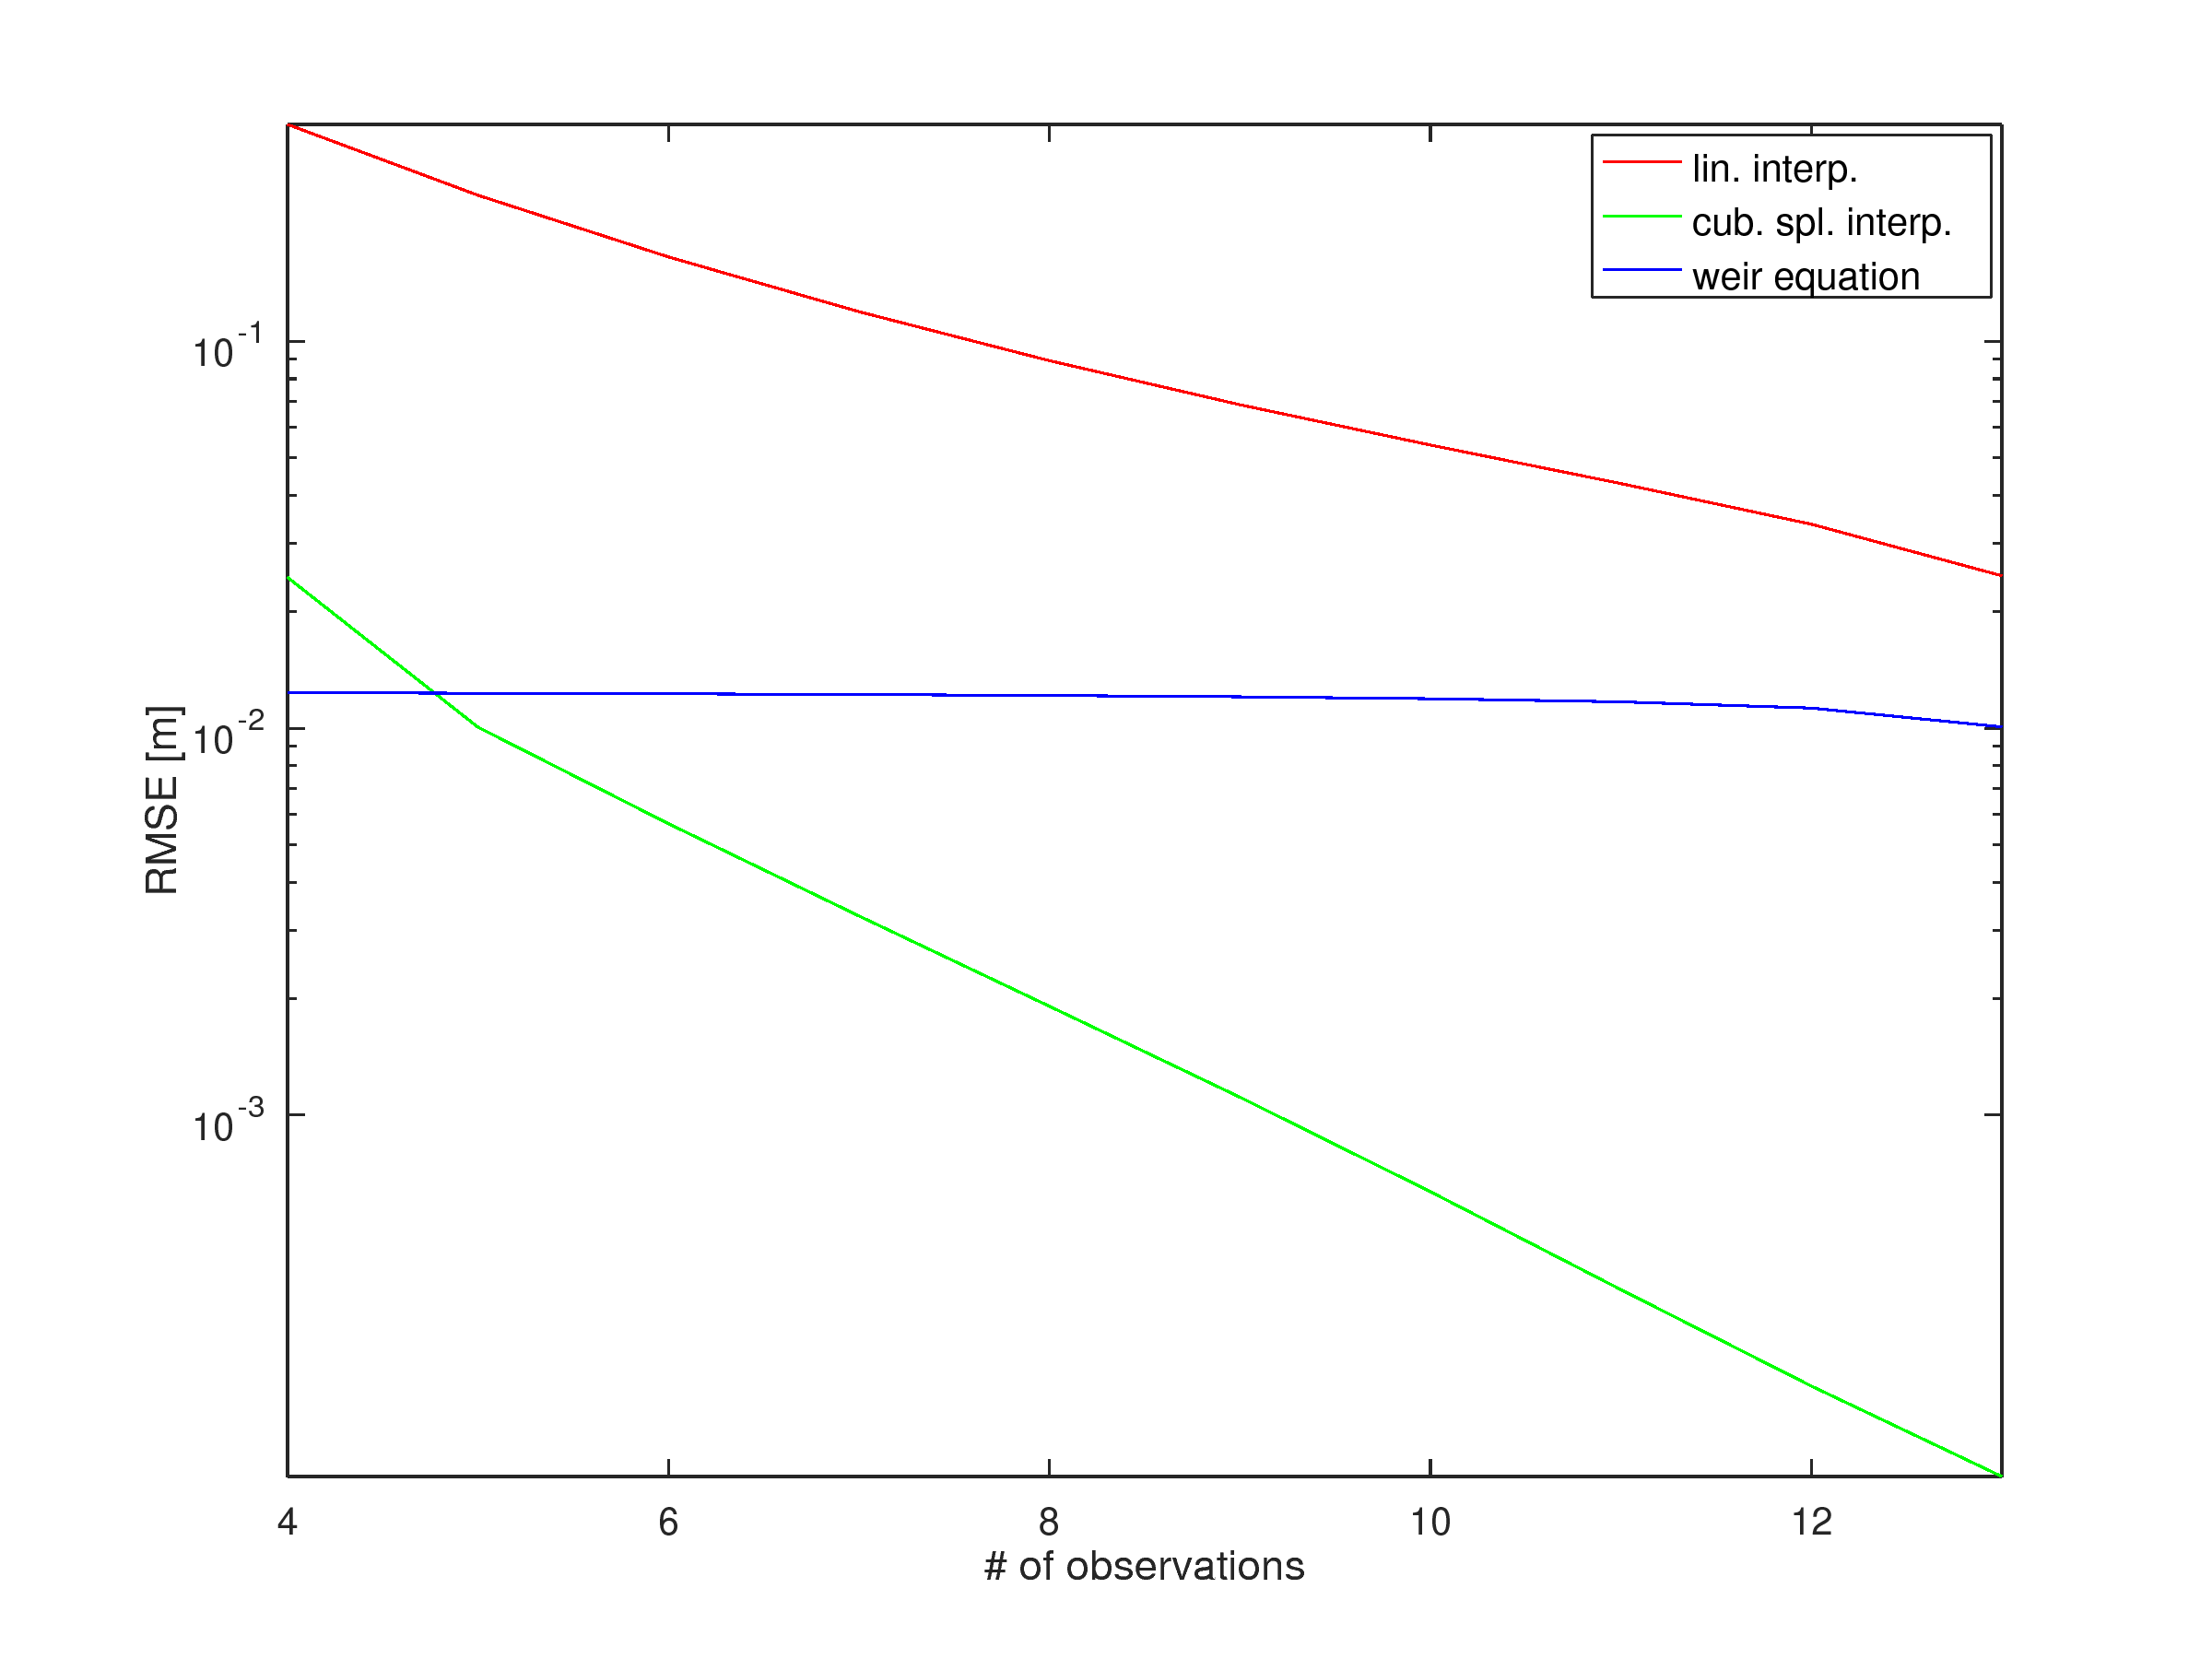
\includegraphics[width=0.7\textwidth]{Figures/fitting_errors.png}
  \caption{Mean RMSE of the three different models as a function of the number of points used to train the models.}
  \label{fig:fitting_errors}
\end{figure}

In Fig.~\ref{fig:fitting_errors} the RMSE obtained by cross-validation as explained in Sec.~\ref{sec:compute_error} are displayed.
No matter how many points are used, the linear interpolation always performs at worst.
By increasing the number of points its performance improves quite rapidly, but not enough to reach that of the other two models.
The process generating the points does not have a linear behavior.
Despite the improvement of its performance, this model will never approximate the process generating the points as well as the others.

The results for the cubic spline interpolation confirm what was already observed in the previous plot.
This is a good model at mimicking the process originating the points.
Its performance goes from slightly worse than that of the weir equation model up to almost \num{2} order of magnitude better.
However, by reducing the number of points, the error of this model increases exponentially.
Thanks to its flexibility, the cubic spline interpolation shows very small errors when fitted with many points.
This model, by definition, interpolates through all of the training points.
If the training points are close to each other, the chance of interpolating an "unseen" point in the middle of two others, or at least to pass very close are very high.
By increasing this distance these chances decrease quite fast, since the cubic spline interpolation is not a very suitable model to describe the behavior of the process between two points.
For this reason the error increases exponentially.

The weir equation model used minimizes the least-square-error of the fit, without necessarily interpolating through the points.
It is a very inflexible model, only two parameters can be varied to improve the quality of fit, while many more observations are available.
For this reason the interpolation through the points cannot be achieved, unless the observations were originated exactly by the model chosen.
The results shown here are the best which can be achieved with it.
Because interpolation cannot be obtained, its error decreases very slowly with increasing number of points.
The inflexibility of this model represents its weakness but at the same time its strength.
This is in fact a very robust model, which still produces good results when few observations are available.
It shows almost no decline in performance by reducing the number of points.

Although its performance is outperformed by the cubic spline interpolation, when more than \num{4} observations are taken, use of this model can still be considered: the error, in spite of being higher than the one obtained with the cubic spline interpolation, is still very little compared with the values of $h$ measured.
In a practical application in hydraulics the difference between the two models could be neglected and one could opt for the most stable one, to stay on the safe side when few points are available.
Fig.~\ref{fig:boxplot_models} in the Appendix summarizes the performance of the three models when using $[\numrange{4}{13}]$ \# of points.
Here it can be seen that the RMSE for the weir equation is higher on average respect to the cubic spline interpolation but still very low (in the order of $\approx \SI{1}{\centi\meter}$).
Its variation is almost inexistent, the box plot is practially described by a line.\\

A closer comparison between the two best models (Fig.~\ref{fig:fitting_std}) shows new interesting features.
The cubic spline interpolation is very sensitive to which points are removed when many are removed.
The standard deviation on its RMSE by changing which observations are removed increases by a factor of \num{60} when \num{4} resp. \num{13} points are used.
The opposite is observed for the weir equation model.
This is more sensitive to which observation is removed when only few of them are removed and becomes less sensitive as fewer observations are used to fit the model.
However, the variation here when \num{4} resp. \num{13} points are used is only $\approx \num{6} \times$.

When considering this, the weir equation can still do better when up to \num{6} points are used, and not just by \num{4} as it was indicated by Fig.~\ref{fig:fitting_errors}.
In the weir equation model proposed by \cite{brown_urban_2009}, the coefficient $C$ varies as a function of $h_w$.
The shorter the weir width, the wider becomes the range of values for the $C$ coefficient.
If a functional relationship $f:h_w \mapsto C$ had been established, then a weir equation model better fitting the data would have been obtained.


\begin{figure}[h]
  \centering
  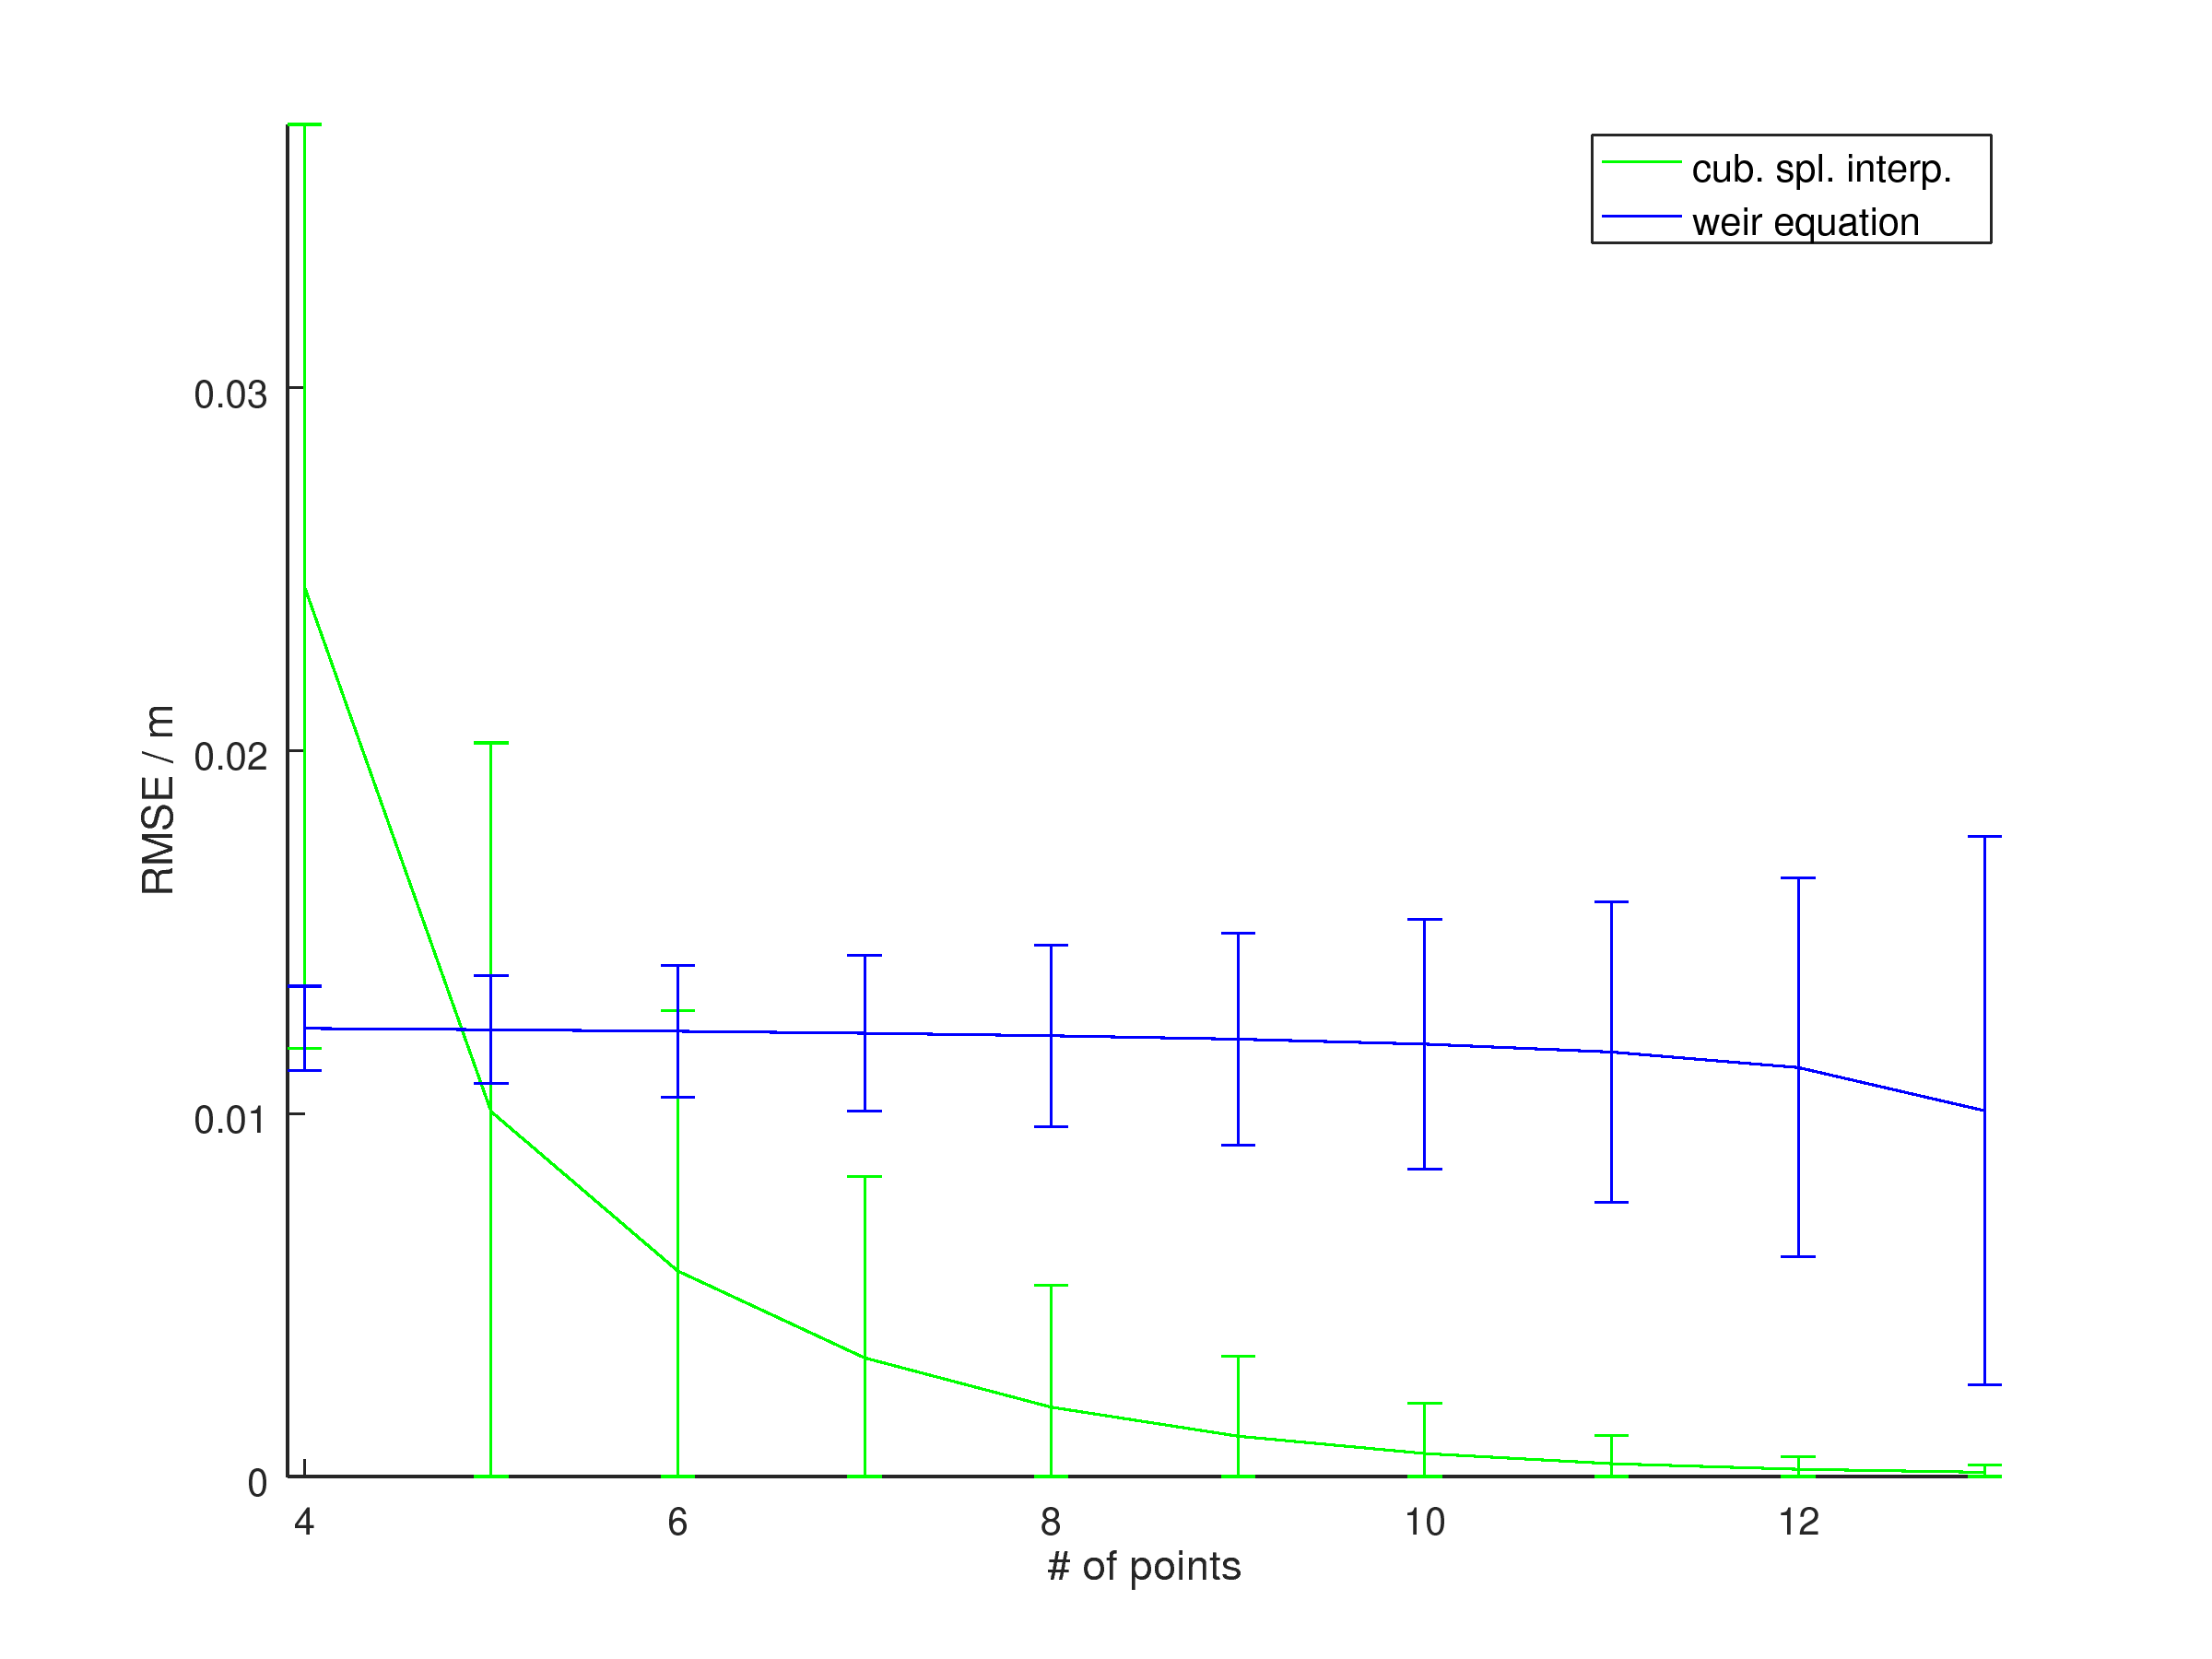
\includegraphics[width=0.7\textwidth]{Figures/fitting_std.png}
  \caption{Closer comparison of the weir equation and the cubic spline interpolation models.}
  \label{fig:fitting_std}
\end{figure}


From this example the importance of the equilibrium \emph{prior knowledge} -- \emph{data availability} can be seen.
Some "interpolation methods" \seb{is it correct "interpolation methods"? how could I call them otherwise?}, e.g. \emph{neural networks} in machine learning (ML), are very data-greedy.
These can perform very well when a big training dataset is available, but fail if not enough data is available.
When obtaining new observations is computationally very costly, like it is the case with most simulations, "interpolation methods" allowing the encoding of prior knowledge can turn out to be very useful.
Gaussian processes (GP) represent a good example.
When the physical laws governing a process are known, i.e. its partial differential equations, it can be tried to encode them in the GP used.
If the information embedded is correct, the result will be very similar to the one observed with the weir equation case study: it does not matter how many points are available to perform the fitting, the results will still be good.
If the right model for the process is found, no more observation are needed.
These are simply given by the evaluation of the model itself.

Moreover the technique just explained can give further insight and can help us learn new functional relationships about the process which is studied.
If the GP chosen performs good, then the functional relationships encoded in it are somehow closely linked with the process itself.
New relationships and dependencies between predictors used and responses observed can be established and we can therefore shed new light on the mechanistic of the process.



%finish with take home message



\seb{should I add a plot of the residues, to see if the weir equation is the "actual model" generating the points?}

%-------------------------------------------------------------------------------
%An \textit{early flood warning tool} in an essential component of an \textit{early flood warning system}.
%An early flood warning system has to be understood as an integrated system of tools and plans to detect and respond to flood emergencies \autocite{icimod_early_2018}.
%This can be managed by the community themselves and if designed, implemented and operated correctly can make the difference between tragedy and survival.

%Such systems have already been installed in various endangered regions in the world.
%After the major flooding of July 2014, the city of Altstätten in the canton of St. Gallen made the decision to install one.
%The system installed uses cameras, sensors and level meters to gather data and information about the current situation \autocite{st._galler_tageblatt_altstatten_2017}.
%When the value of certain parameters exceed the given threshold, a dangerous situation is recognized and the alarm signal is sent.

%Three years after the installation of the system an alarm rings in the middle of the night.
%Firemen go immediately into action in order to install temporary measures to fight against the water.
%A couple of hours later the torrent overflows at several points and the city gets flooded.
%Damages are less severe than last time, especially thanks to the temporary measures installed, but possibly they could have been reduced even more.

%Crucial in order to limit the damages is the intervention time before the actual flooding occurs.
%The earlier the dangerous situation can be detected the more time is available to the population and authorities to get ready and set up different types of temporary mitigation measures.
%Systems based on sensors monitoring the evolution of the current situation in the upper part of the catchment are quite reliable but do not allow for long anticipation time.

%Numerical simulations can be run with meteorological forecast data and approximate soil saturation conditions in order to obtain early predictions of the event outcome.
%However, the big advantage of predicting with that much anticipation is partially lost due to the duration of such simulations.
%Accurate meteorological forecasts are available only few hours before the event.
%If the model require several hours to run, which is often the case to obtain accurate predictions for catchments of this extent, then the advantage of being able to run it in advance is canceled.

%A possible solution to this problem is the development of an \emph{early flood warning tool} based on an \emph{ad hoc surrogate model} exploiting the catchment specific behavior.
%This early flood warning tool should be able to recognize if a rain event will generate a channel discharge leading to flooding and if yes within how much time.
%For this scope two different emulators are used.
%The first emulator classifies a rain event based on the forecasted \emph{average rain intensity} and \emph{current soil saturation} into two groups: rain events generating discharge exceeding a chosen threshold ($Q_!$) and rain events not generating discharge exceeding the threshold.
%For events exceeding the threshold a second emulator is developed.
%This predicts the time the rain event will need to produce the threshold discharge $Q_!$ at the outlet of the catchment.
%-------------------------------------------------------------------------------


\newpage

\noindent{\LARGE\textbf{Case study 2}}
%===============================================================================
\section{An hydrological emulator: estimating the \textit{time-to-threshold}}
%===============================================================================

With this case study it was decided to address a complex hydrological problem by means of emulation.
The problem we want to solve is estimating the time needed for a channel conveying water from a catchment to reach a certain threshold discharge ($Q_!$) at its outlet as a function of rain intensity and initial soil saturation.

For the experiment a synthetic catchment topography was used, which at first glance can make the case study look very abstract.
In reality the emulator is just exploiting the catchment specific behavior, which is of course different from one catchment to another, but the methodology applied here could be applied to whatever catchment.
The emulator developed here, with the appropriate adjustments, could be exploited as an \emph{early flood warning tool}.

As for the previous example, the simulations were run with the open source software \textit{FullSWOF\_2D-v.1.07.00} \autocite{delestre_fullswof:_2014} \seb{put the citation every time that it is mentioned?}, while the input files necessary for the simulations were prepared with \textit{GNU Octave 4.2.1} \autocite{octave_community_gnu_2018} \seb{how to cite this?} with the aid of the package \textit{fswof2d}.


%-------------------------------------------------------------------------------
\subsection{Material and methods}
%-------------------------------------------------------------------------------
%...............................................................................
\subsubsection{Generating the topography}
%...............................................................................

The topography used represents a catchment of size $\SI{2}{\kilo\meter} \times \SI{2}{\kilo\meter}$ and it is visible in Fig.~\ref{fig:topography}.
It is composed of a sloping plane with three Gaussian bumps on the top.
The Gaussian bumps have different heights and widths and generate a \emph{Y-shaped channel} which extends from the upper and left boundary down to the lower boundary.
A paraboloid was added to the plane to promote the accumulation of water in the channel.
This has a single outlet located close to the center of the domain's bottom boundary.

The synthetic topography produced, in contrast to a real one, has the advantage of having a much smoother surface, which allows using a coarser grid resolution without losing topographical features.
The coarser the grid the fewer the nodes where the finite volume (FV) equations have to be solved, which reduces the simulation runtime \seb{how does it decrease? linearly? quadratically?}. 
Another advantage of having a smooth topography, not presenting discontinuities, is that the solutions converge easily, and no grid refinement is necessary.
The grid used is composed of $\num{100} \times \num{100}$ cells, giving a resolution of $\SI{20}{\meter} \times \SI{20}{\meter}.$

\begin{figure}[h]
  \centering
  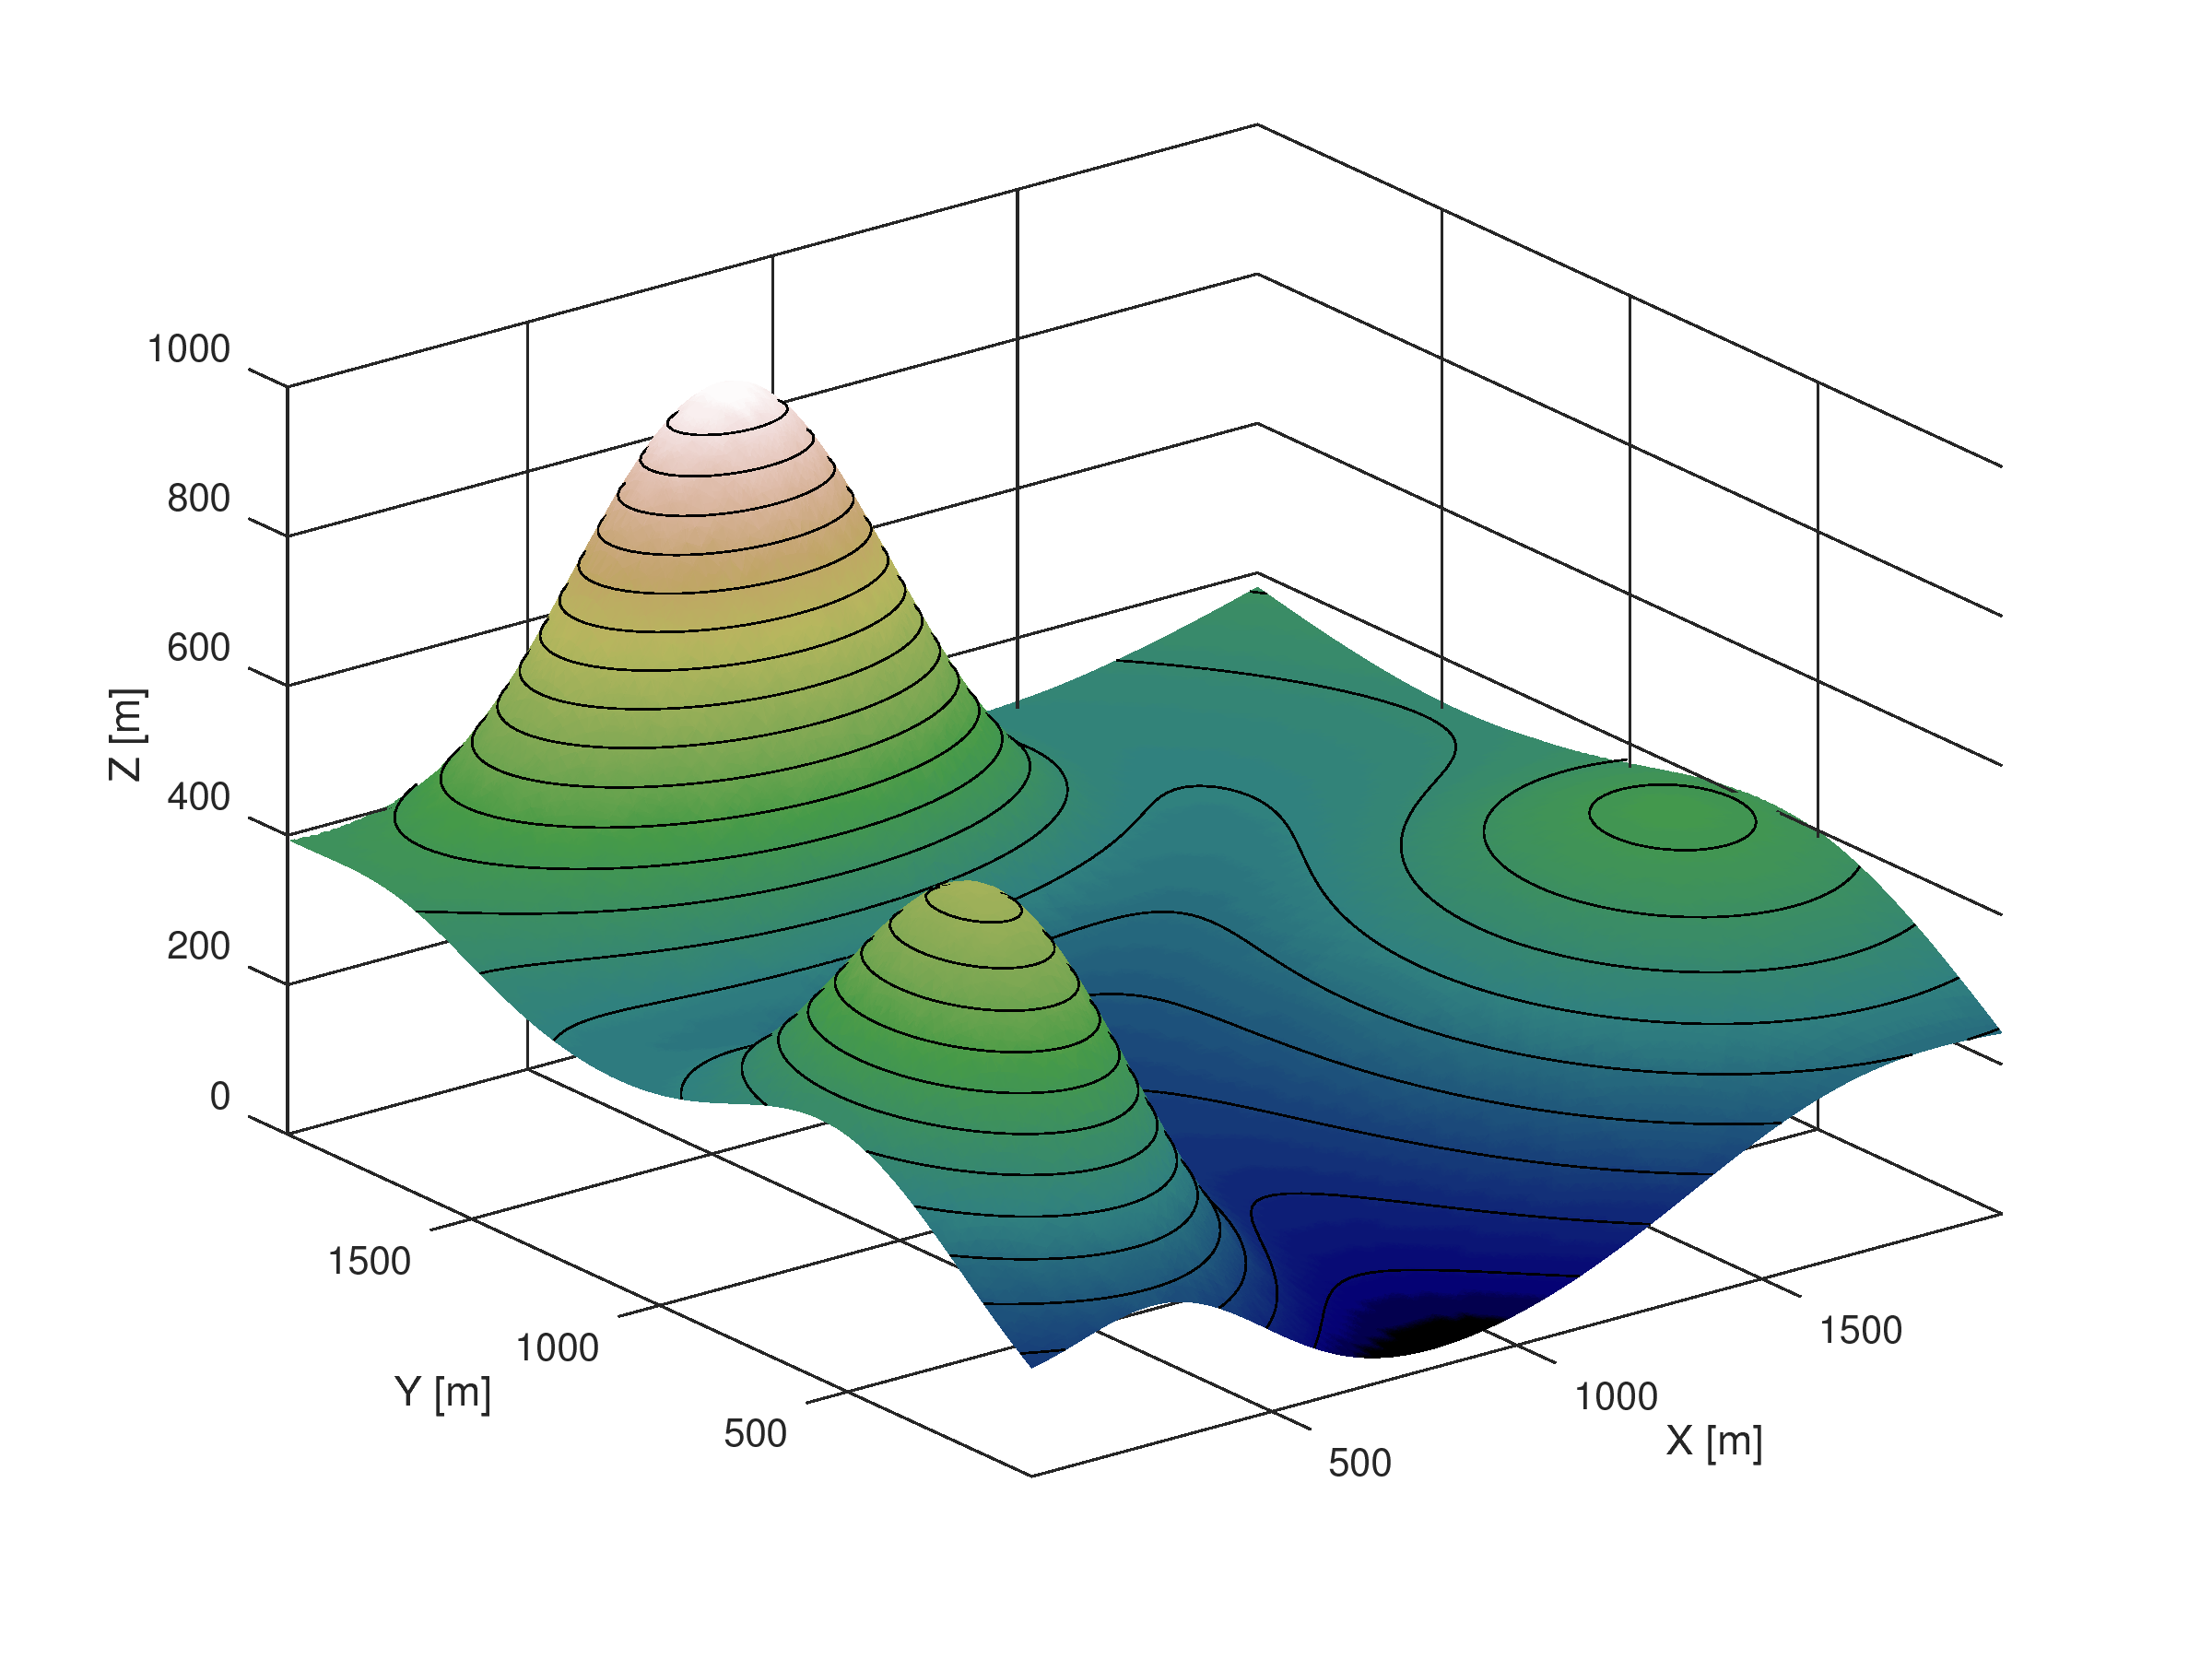
\includegraphics[width=0.7\textwidth]{Figures/topography.png}
  \caption{Synthetic topography composed of three Gaussian bumps on a sloping plane.}
  \label{fig:topography}
\end{figure}

%...............................................................................
\subsubsection{Setting-up the simulations}
%...............................................................................
The dataset required for building the emulator was generated by running \num{50} simulations with different combinations of the variables \emph{rain intensity} ($I$) and \emph{initial soil saturation} ($\theta_i$).
The initial soil saturation, being a spatially distributed variable, was kept uniform over the whole domain.
The rain intensity was kept constant and was uniformly applied over the domain, also since \textit{FullSWOF\_2D}, at this stage of development, only allows for uniformly distributed rain events \autocite{laguerre_documentation_2016}.

\num{5} different initial saturations in the $[\numrange{0}{1}]$ interval and \num{10} rain intensities in the \SIrange{10}{35}{\milli\metre\per\hour} interval were taken and all their possible combinations were used as inputs for the simulations.
The rain duration was set to \SI{6}{\hour}, while a simulation duration of \SI{9}{\hour} was chosen in order to be able to observe the hydrograph recession. A time resolution of \SI{60}{\second} was used, which means that intermediate simulation results were written to the \emph{outputs} file every \SI{60}{\second}.

Some parameters, namely those specific for the catchment in questions, were kept constant over all of the simulations.
These are summarized in Tab.~\ref{tab:simulations_parameters}.
The parameters marked with * are those \emph{spatially distributed}, meaning that a different value could be set for every cell.
For simplicity, a spatially uniform catchment was used, therefore the values from the table are valid for the whole domain.
Three \textit{wall boundary conditions} were set, for the upper and the two lateral boundaries.
For the bottom boundary a \textit{Neumann boundary condition} was selected, allowing water to freely outflow through that boundary and making sure that all of the water is lost from here.

\begin{table}[h]
  \centering
  \caption{Parameters and setting fixed for all simulations.}
  \label{tab:simulations_parameters}
  \begin{threeparttable}
    \begin{tabular}{lrl}
      \toprule
      \textbf{Parameter} & \textbf{Value} & \textbf{Units} \\
      \midrule
      Domain x-length                          &    $2'000$           & \si{\meter}   \\
      Domain y-length                          &    $2'000$           & \si{\meter}   \\
      Number of cells x                        &    $100$             & --   \\
      Number of cells y                        &    $100$             & --   \\
      Friction coefficient\tnote{*}            &    $0.03$            & \si{s.m^{-1/3}}\\
      Crust thickness\tnote{*}                 &    $1$               & \si{\meter}\\
      Crust hydraulic conductivity\tnote{*}    &    $2\cdot 10^{-6}$  & \si{\meter\per\second}\\
      Soil hydraulic conductivity\tnote{*}     &    $2\cdot 10^{-6}$  & \si{\meter\per\second}\\
      Soil suction head\tnote{*}               &    $0.09$      & \si{\meter}\\
      Soil maximum infiltration rate\tnote{*}  &    $19.8$      & \si{\milli\meter\per\hour}\\
      \bottomrule
    \end{tabular}
    \begin{tablenotes}
      \item[*] Parameters spatially distributed.
    \end{tablenotes}
  \end{threeparttable}
\end{table}

%...............................................................................
\subsubsection{Extracting the datasets}
%...............................................................................
This data constitute the \emph{training} dataset for the emulator.
A \emph{test} dataset and a \emph{validation} dataset were also generated and can be found in the Appendix~\ref{Appendix}. \seb{verify if they are really added}

The datasets used to build the emulator was extracted from the simulation outputs.
The extraction was done in two steps.
In the first step the outflow hydrographs were extracted from the output data. 
This was done by summing up the cell discharge along the whole domain bottom boundary for every saved time-step (one value every \SI{60}{\second}).
Result of this operation is a discharge values time series of \num{540} elements.
The same procedure was repeated with every one of the \num{50} experiments.

Fig.~\ref{fig:hydrographs3d} shows the extracted hydrographs.
Here many interesting features can be observed.
First of all it can be seen that experiments run with the two lowest rain intensities and low initial soil saturation generated no discharge.
In the second place, simulations run with $\theta_i = \num{1}$ always reached their peak discharge, and this happens quite quickly.
Some of these show a second smaller increase after the first quick rising limb.
This gets higher the higher the rain intensity.
Some simulations show two "increase bumps" after the first rising limb.
This effect is due to the topography.
The topography used presents zones with very steep slopes and others with very flat ones.
This causes that water droplets at the same distance from the outlet to reach it with different travel times.
When the water from the inclines has reached the outlet, that coming from flat areas is still traveling downstream.
After a given lapse of time this water reaches the outlet as well, giving rise to the bumps visible in the hydrographs.\\

\begin{figure}[h]
  \centering
  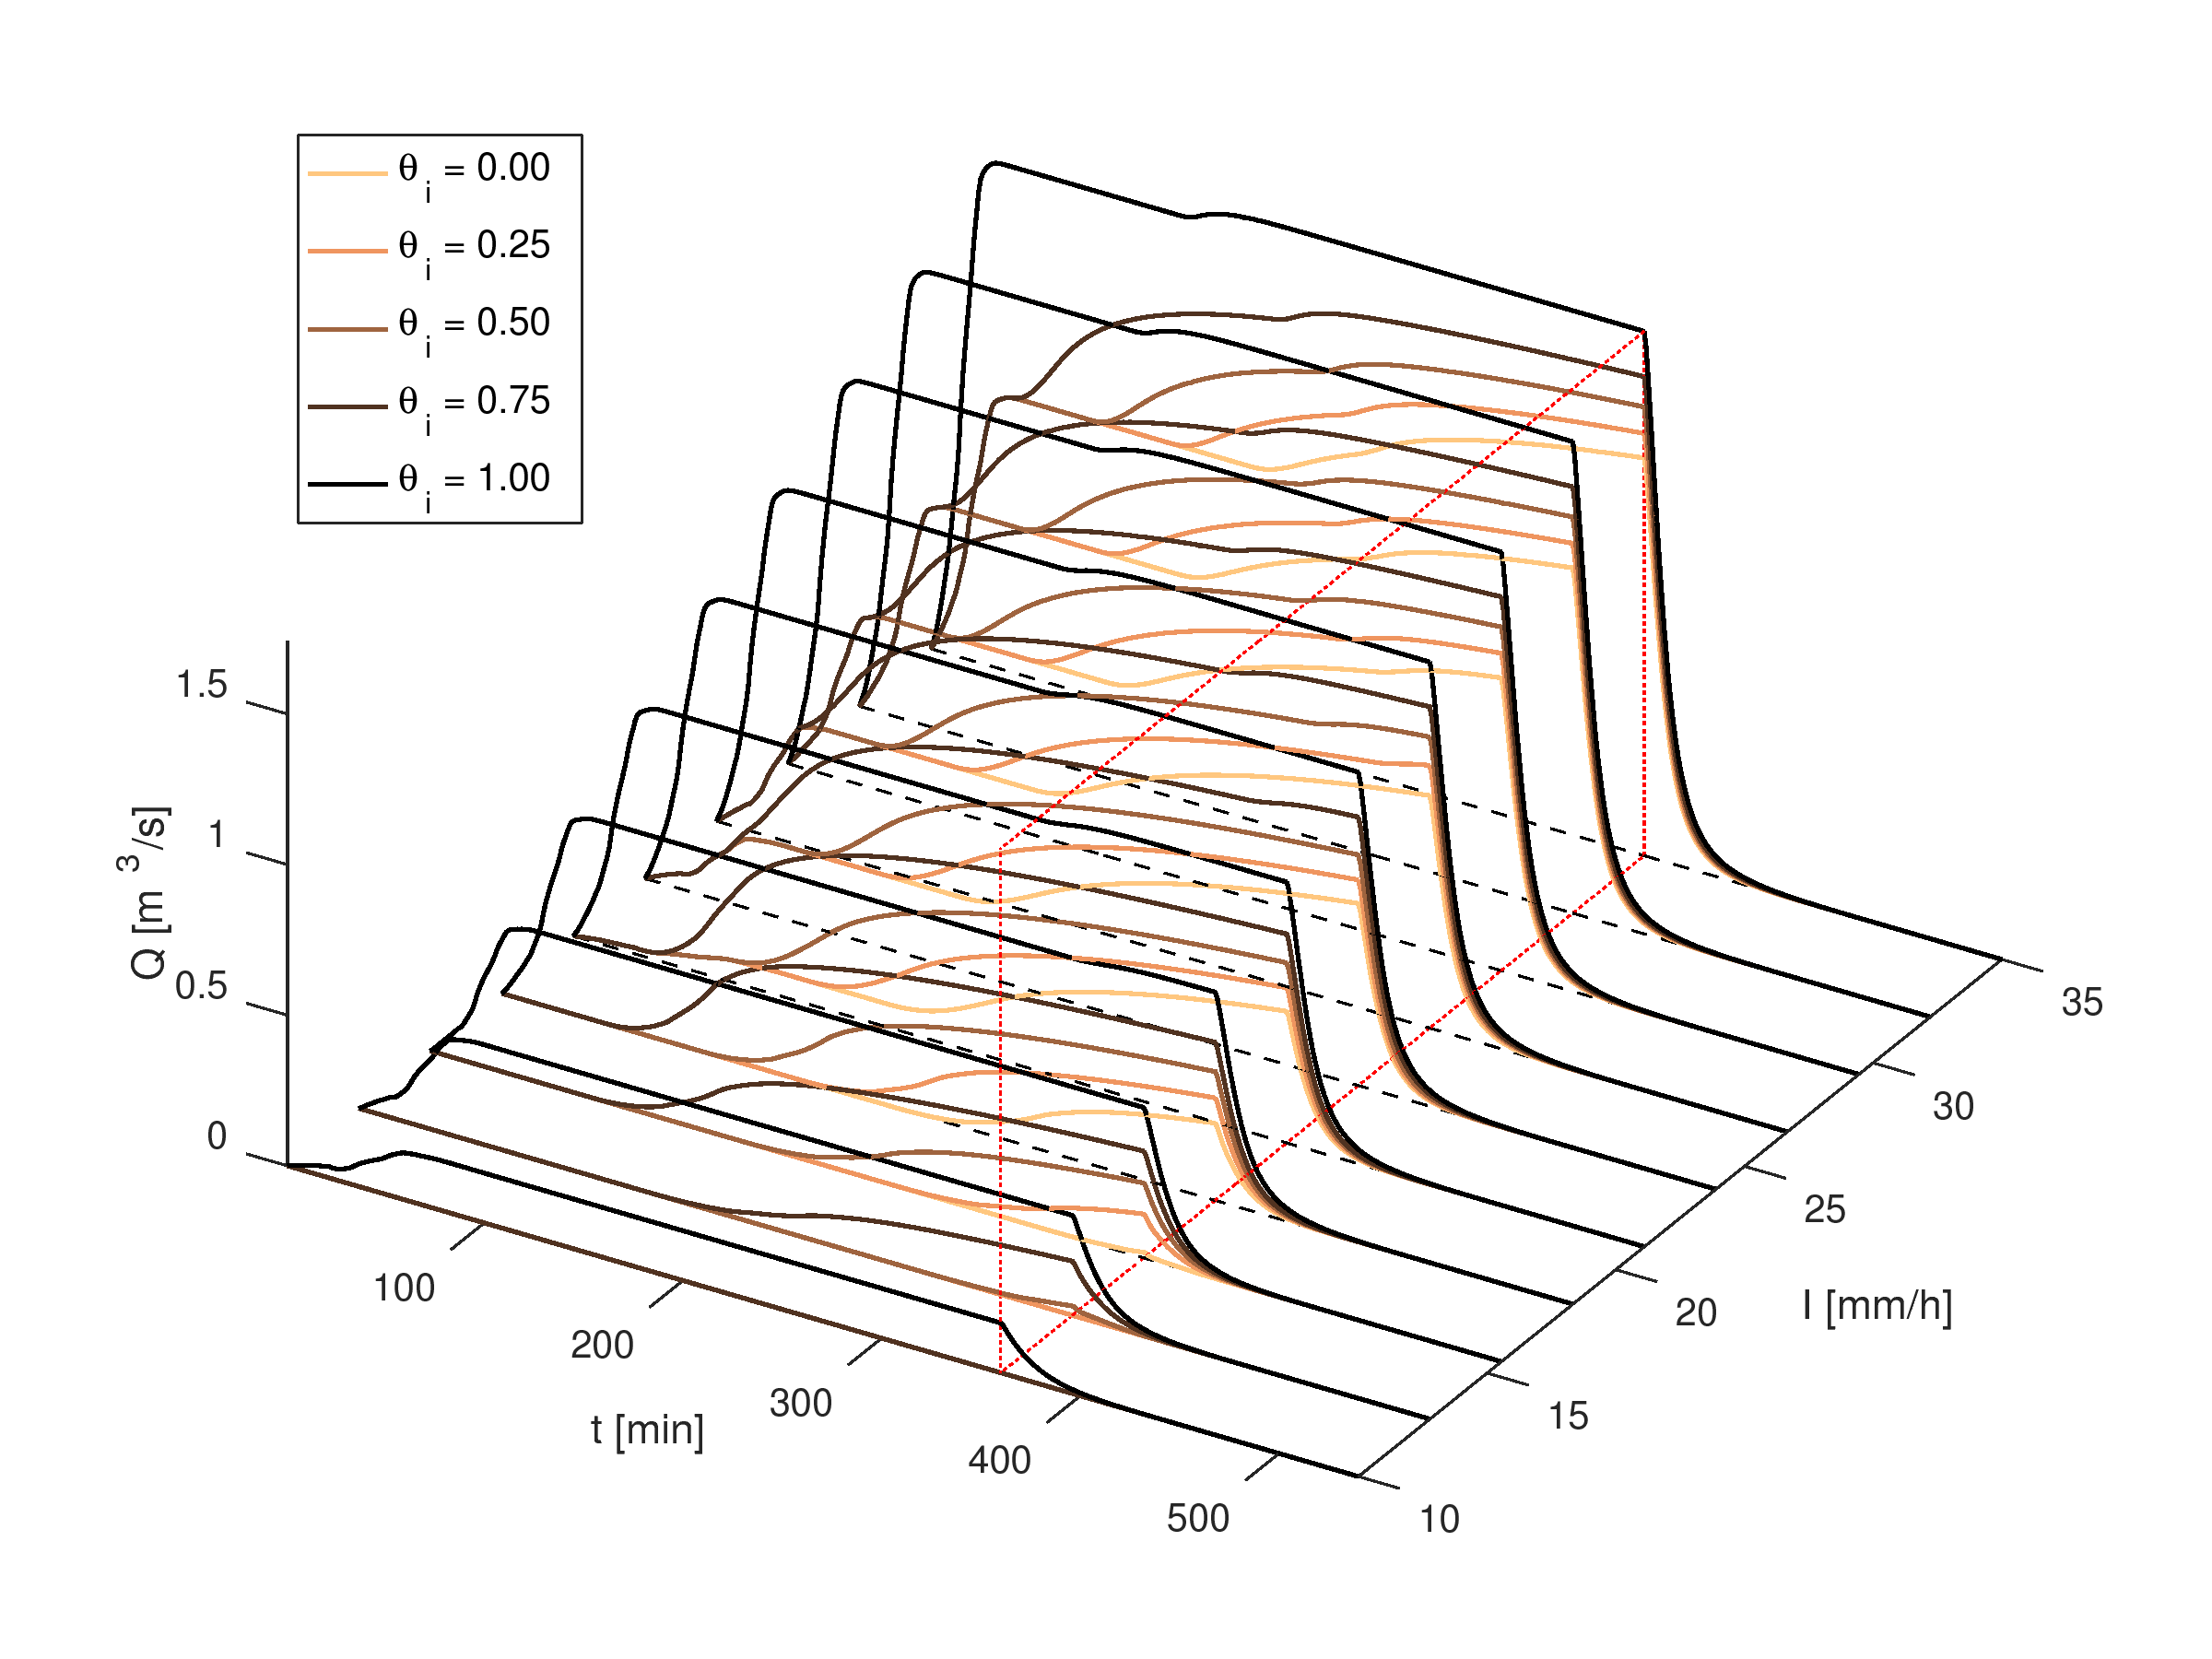
\includegraphics[width=0.75\textwidth]{Figures/hydrographs3d.png}
  \caption{Response hydrographs for the \num{50} simulations at the catchment outlet. The red frame shows the end of the rain event. Depth-dimension shows the \emph{rain intensity} variable, while the \emph{initial saturation} variable is rendered by the colormap.}
  \label{fig:hydrographs3d}
\end{figure}

To build the \emph{time-to-threshold emulator}, the emulator giving the arc of time $t_!$ passed from the beginning of the rain event to the exceeding of the threshold discharge $Q_!$, a threshold discharge has to be established.
For a real case study a characteristic discharge value would be set.
This could be the discharge at which a bridge or the embankments downstream of the considered domain are overflown.
Here this value can be chosen with greater freedom, and the effects of choosing different values can be studied.

By looking at the hydrographs of Fig.~\ref{fig:hydrographs3d} it can be observed that $t_!$ is a difficult quantity to predict.
In fact, depending on the $Q_!$ set, there is a variable number of experiments not reaching the threshold, of experiments reaching it very quickly, or of experiment with similar conditions but very different $t_!$.
Especially this last point can be better understood by comparing Fig.~\ref{fig:hydrograph}.
The quantity $t_!$ shows discontinuities.
Within the region defined by the $Q_!$ and the $Q'_!$ lines the hydrograph presents a plateau.
Here, a minimal variation of the threshold set can make the time-to-threshold fall towards $t_!$ or $t'_!$, hence causing a big jump in the value.

\begin{figure}[h]
  \centering
  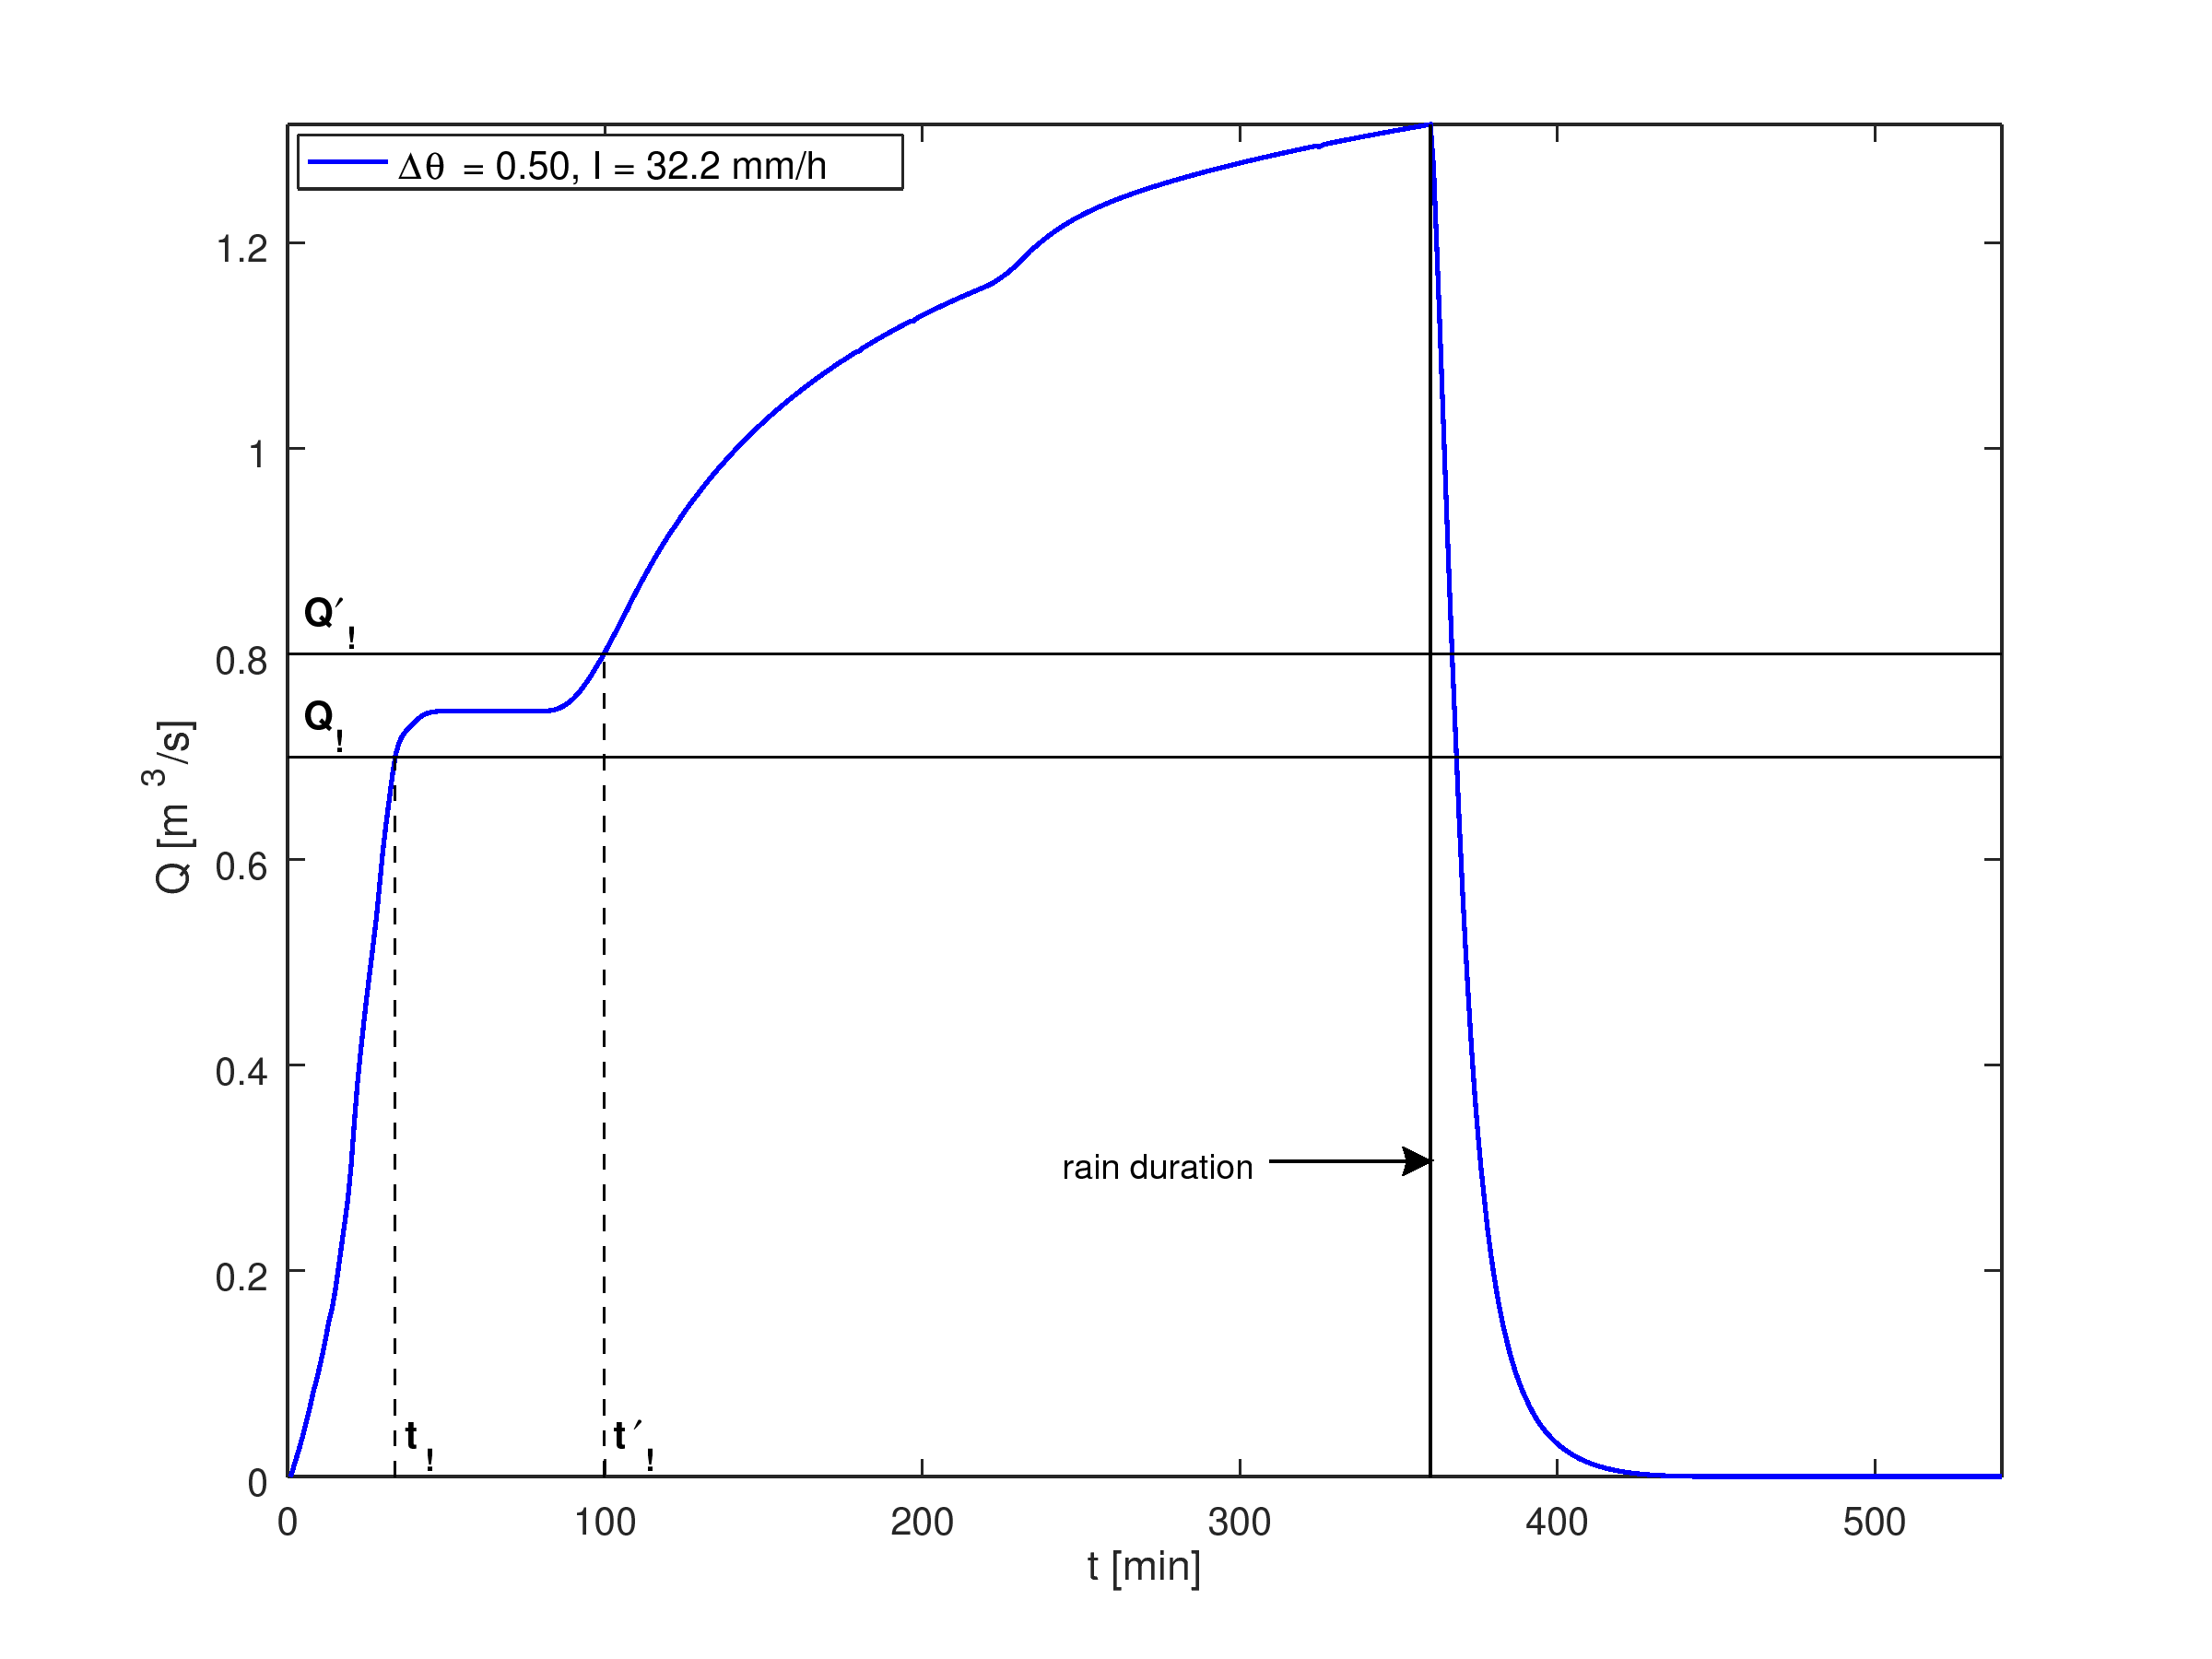
\includegraphics[width=0.7\textwidth]{Figures/hydrograph.png}
  \caption{Response hydrograph for $\theta_i = \num{0.5}$ and $I = \SI{32.2}{\milli\meter\per\hour}$. The discontinuity in the quantity $t_!$ is visible between the $Q_!$ and the $Q'_!$ lines, where the discharge presents a plateau.}
  \label{fig:hydrograph}
\end{figure}

$Q_!$ was set to \SI{10}{\percent} \seb{why this value? should I give any explanation?} of the $Q_{max}$ value recorded, corresponding to \SI{0.17}{\cubic\meter\per\second}.
The time at which this value is exceeded for the first time was extracted from every hydrograph and forms the dataset for the \emph{regression emulator}.
Another dataset for the \emph{classification emulator} was created by assigning the value \num{-1} to rain events not reaching the threshold and \num{1} to all of the others.


\subsubsection{Building-up the classification emulator}


\subsubsection{Building-up the regression emulator}


%-------------------------------------------------------------------------------
\subsection{Results and discussion}
%-------------------------------------------------------------------------------

\begin{itemize}
\itemsep0em
  \item emulator should never underestimate danger (what type of error is this? we want to avoid it absolutely)
  \item try to perform GP interpolation. If it does not work, explain why polynomial interpolation (no time)
  \item use emulator with uncertainty in the $I$ and $\theta_i$. Perform uncertainty quantification
\end{itemize}


\subsubsection{Classification emulator}

Results for the classification emulator
\begin{itemize}
  \item show classification with 3 different $Q_!$
  \item perform testing 
\end{itemize}

\begin{figure}[htpb]
  \centering
  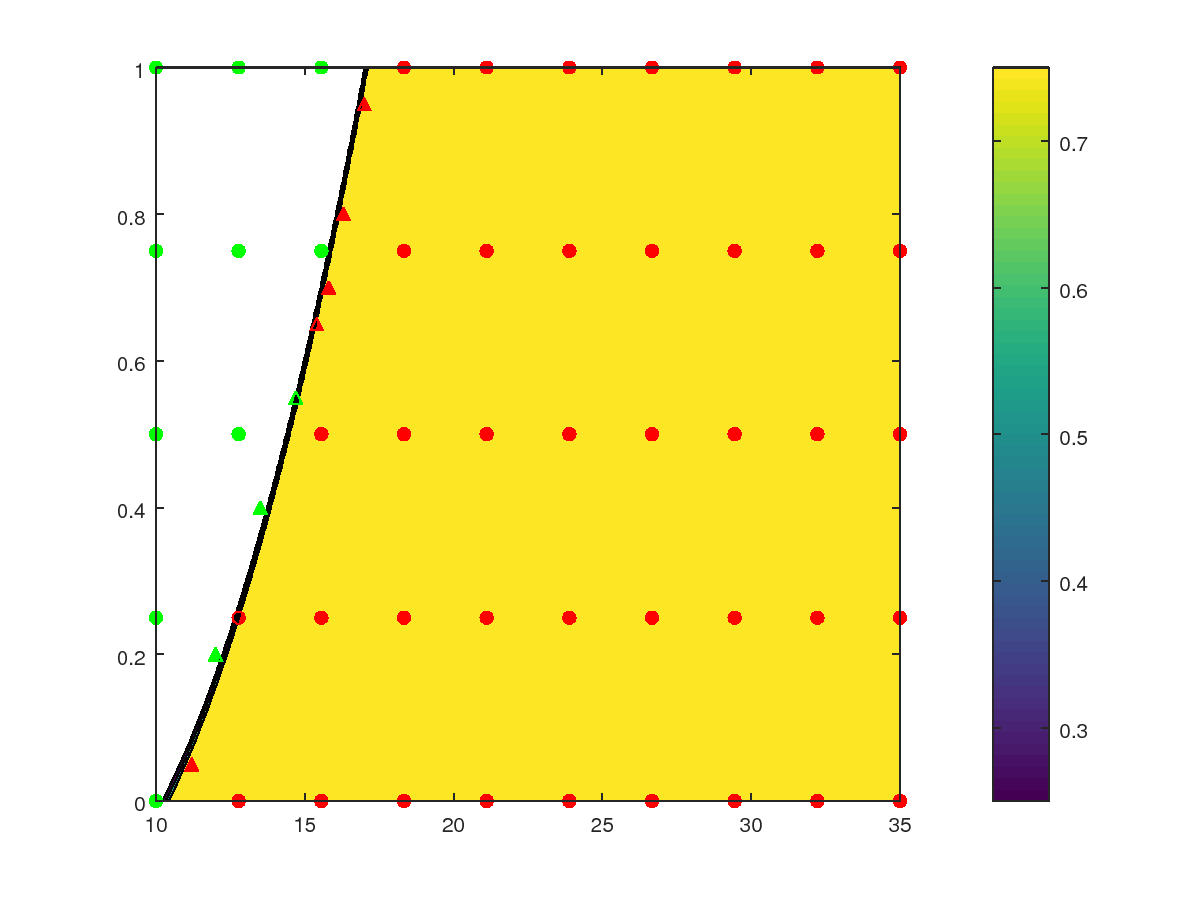
\includegraphics[width=0.75\textwidth]{Figures/classification.png}
  \caption{Binary classification emulator: events reaching $Q_!$ (red) and events not reaching $Q_!$ (green) for $Q_! = XX.X$.}
  \label{fig:classification_Q1}
\end{figure}


\subsubsection{Regression emulator}

\begin{figure}[htpb]
  \centering
  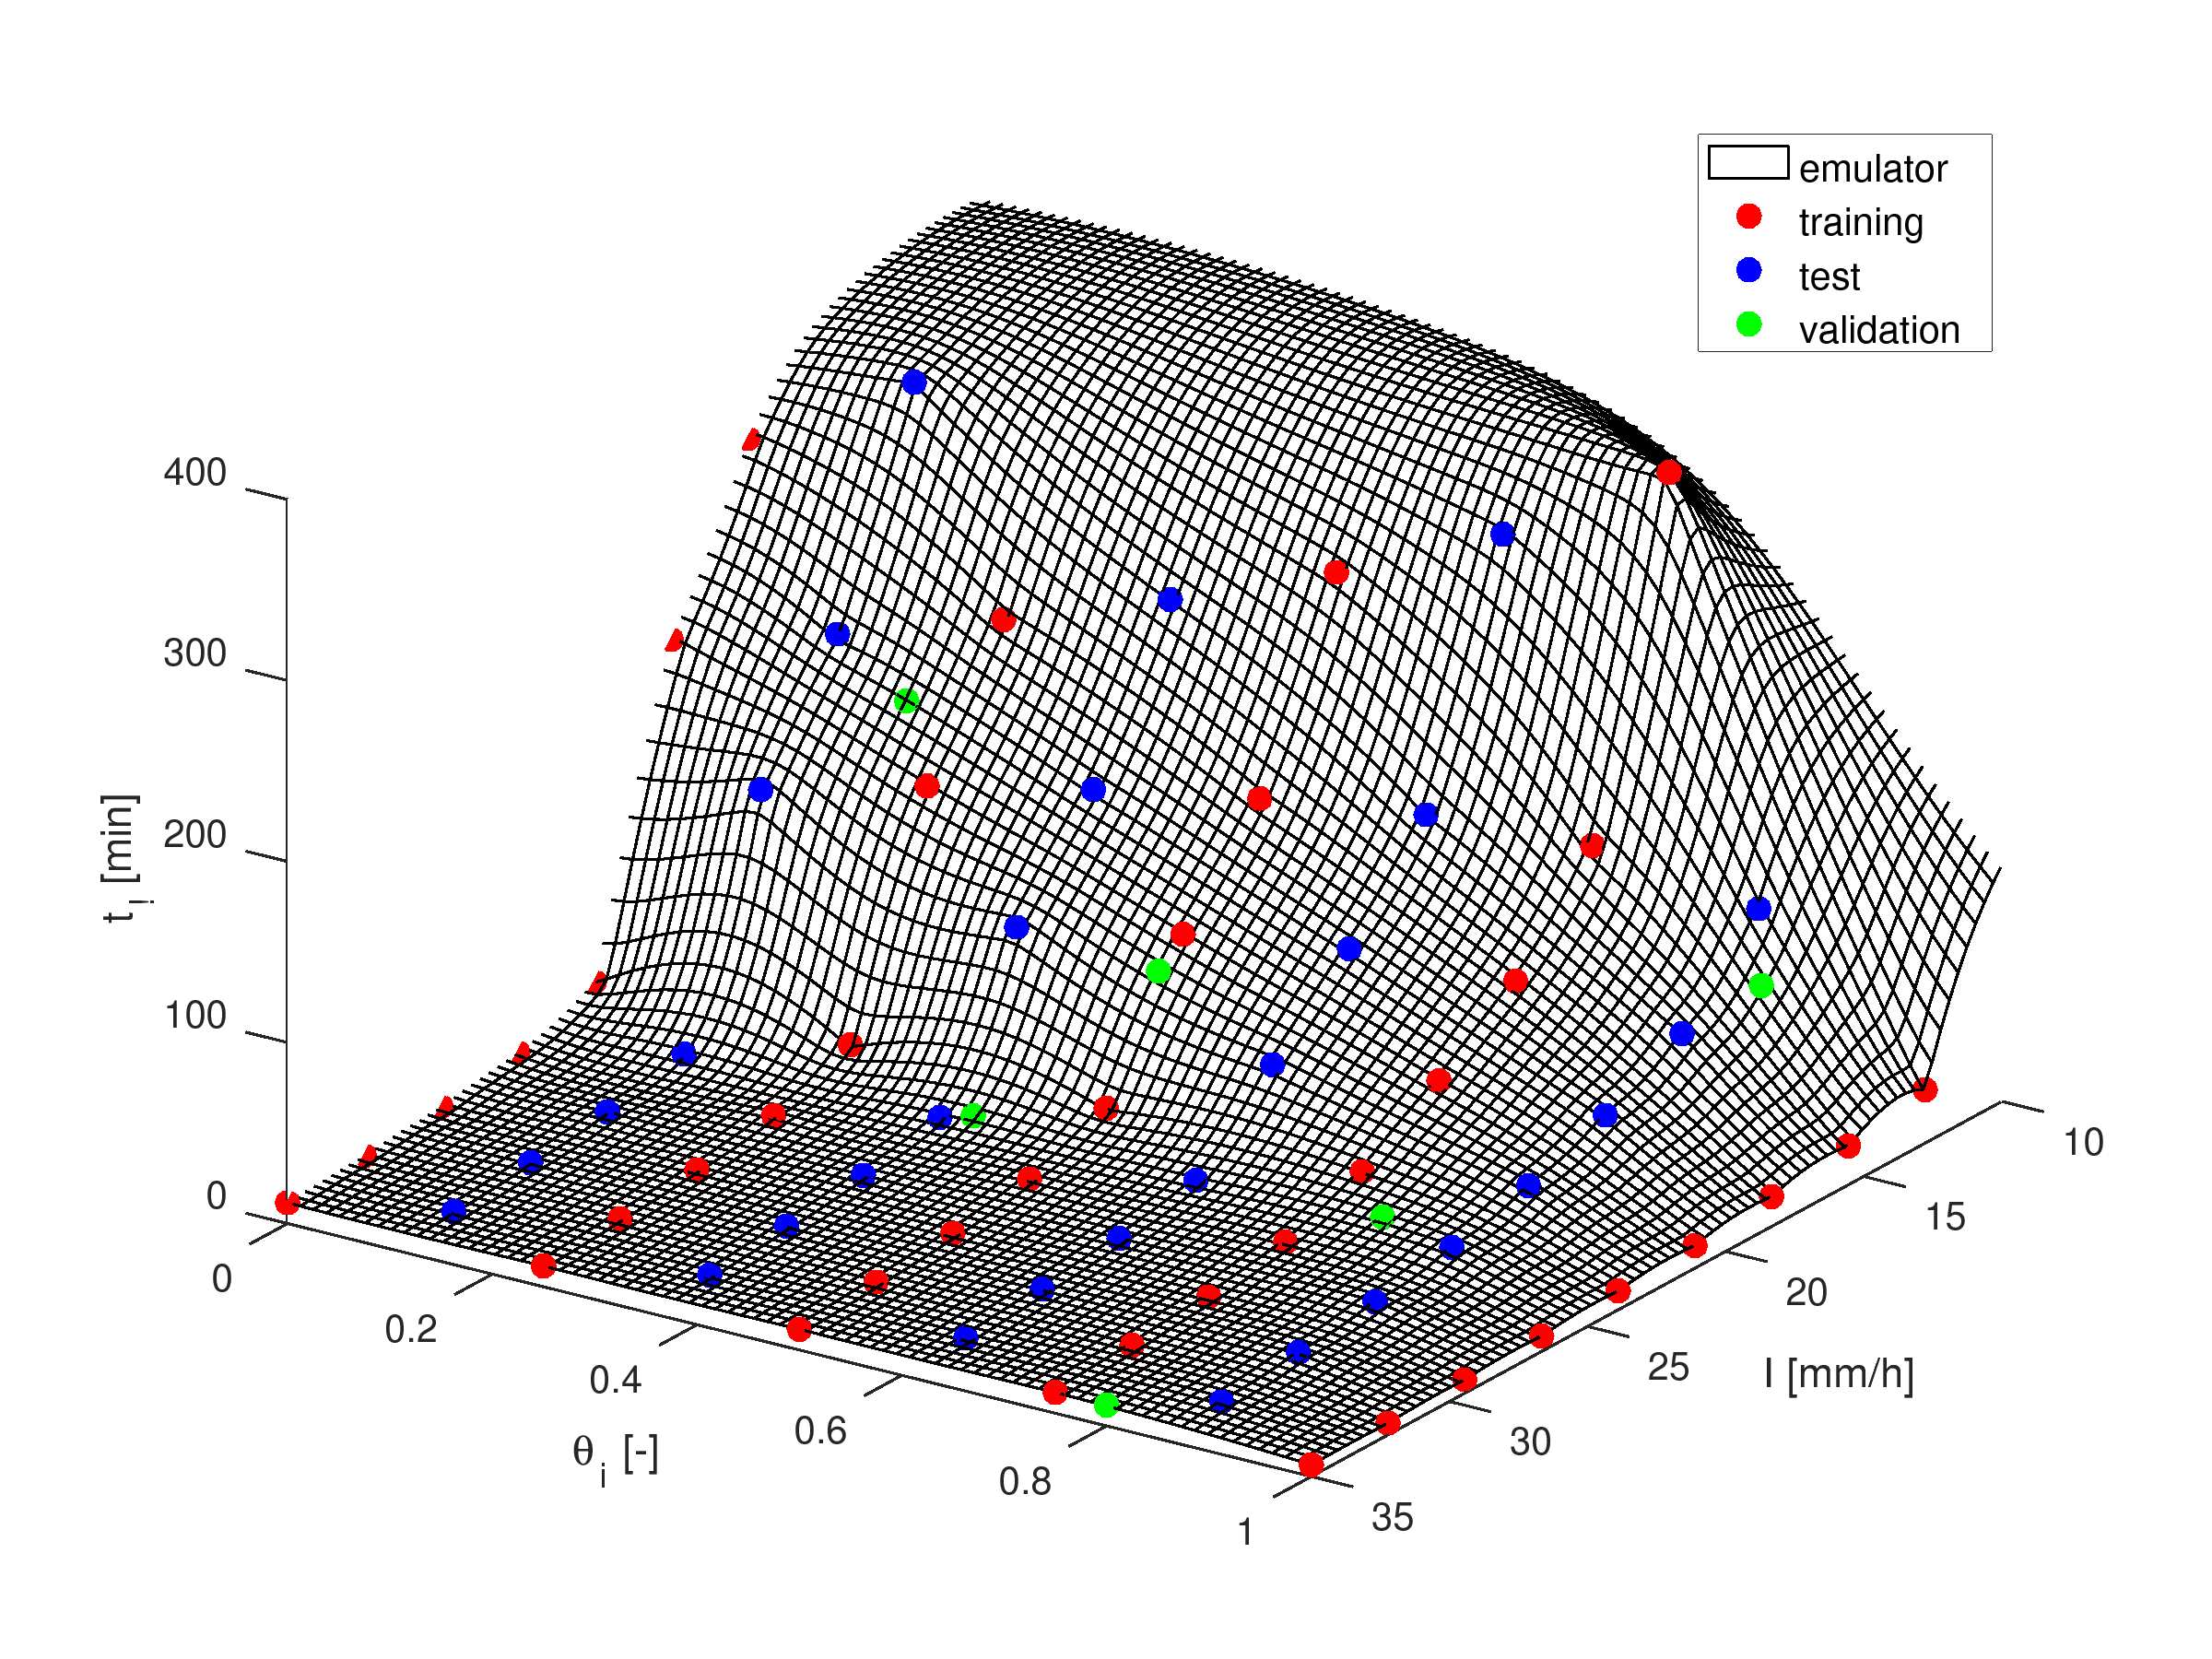
\includegraphics[width=0.7\textwidth]{Figures/emulator.png}
  \caption{Time-to-threshold emulator: training (red), test (blue) and validation (green) datasets and the emulator producing the intrapolation response.}
  \label{fig:regression_emulator}
\end{figure}


\begin{table}[htpb]
  \centering
  \caption{Emulator performance on \emph{test} and \emph{validation} data}
  \label{table label}
  \begin{tabular}{lcc}
    \toprule
     & \textbf{MAE [\si{\minute}, \si{\percent}]} & \textbf{RMSE [\si{\minute}, \si{\percent}]} \\
    \midrule
    \textbf{test} & val & val \\
    \textbf{validation} & val & val \\
    \bottomrule
  \end{tabular}
\end{table}


\chapter{Discussion}
\label{chp:conclusions}



\chapter{Conclusions}
\label{chp:outlook}




%individual results are probably being discussed in 3.1.2 and 3.2.2

%Here, you could provide a joint discussion, maybe discussion common features/insight for both case studies. FullSwof, GPs as tools vs. "simple" emulators such as response surfaces/lin. methods.

%Also, you could move the next steps/outlook part here.



%probably move bullet points 2 and 3 to discussion section and have Conclusion as summarizing section, re-stating the problem, the general approach, the main results (Answers to Research questions). and brief summary of future work.


%5.1. Answers to research questions

%5.2. Open questions


%s of this thesis.

%You can stay with "Goals", or break it down into different "objectives"/sub-goals, if needed.

%From goals/objectives, usually research questions are derived. These should be as specific as possible, so you can write a concise answer.





%The work done on emulation 

This thesis follows a storyline, which connects up the dots, resulting in a prelude to emulation for near-time flood prediction.
Venturing in a completely new field, that of emulation, opened me up a whole new world.
This itinerary through emulation, after clearing up some initial doubts, made me realize its true potential.
Emulation can have great applicability, especially in the engineering fields.
Engineering often has to tackle repetitive problems, which solution can be found only iteratively.
Emulation can provide alternative new ways to solve such problems.
Once an appropriate emulator for a specific task is built, this can provide fast answer to the problem of interest.
Emulation can be performed at almost no cost: it requires neither special tools nor special investments.
The work done on this thesis demonstrate it.\\

In spite of its simplicity, the first case study was for me a very didactic one.
The weir equation, commonly used in hydraulic engineering, proved to be a fair approximation of the relation discharge-height over the weir, although flexible non parametric interpolation techniques have shown to produce more accurate estimates when an adequate number of observations is available.
This case study also shows the potential of numerical simulation in replacing the realization of laboratory experiments, with the potential of reducing future research costs and time.\\

Although the methodology in the second case study appears more complex than the one adopted in the first one, the high level of abstraction and generalization of the presented workflow allows to apply the proposed early flood warning system to real situations with only slight modifications. These especially concerns the assessment of the emulator performance. Still, the partial accuracy assessment conducted reported excellent performance, especially with regards to the estimation of the time period before a flood occurs. \\

In conclusion, this thesis shows the benefit of conjugating the accuracy of numerical simulation with the huge enhancement in computing time provided by emulators. In the engineering field, promising research areas may include uncertainty propagation, sensitivity analysis and models optimization or calibration, which are actually hampered by the excessive computational burden of numerical simulation. 


 
% - automatization
% - to bridge a gap
% innovation

 
 

 




















%-------------------------------------------------------------------------------
%  BIBLIOGRAPHY
%-------------------------------------------------------------------------------

\printbibliography[heading=bibintoc] \seb{any rule for the bibliography? print ISBN? print url where document is available (if pdf)?}

%-------------------------------------------------------------------------------
%  APPENDIX
%-------------------------------------------------------------------------------

\appendix % Cue to tell LaTeX that the following "chapters" are Appendices

% Include the appendices of the thesis as separate files from the Appendices folder
% Uncomment the lines as you write the Appendices

% Appendix
\chapter{Appendix}


\seb{change appendix name or way it is displayed. I want to have just 1 appendix}
%===============================================================================
\section{Additional material}\label{sec:additional_material}
%===============================================================================
\noindent The \citetalias{octave_community_gnu_2018} fswof2d package can be downloaded at:
\begin{itemize}
\itemsep0em
  \item \url{https://bitbucket.org/binello7/fswof2d/}
\end{itemize}

\noindent All of the material composing these thesis (documents, scripts, files, functions, etc.) is available at:
\begin{itemize}
\itemsep0em
  \item \url{https://bitbucket.org/binello7/master_thesis}
\end{itemize}



%===============================================================================
\section{Case study 1}
%===============================================================================
\begin{figure}[H]
  \centering
  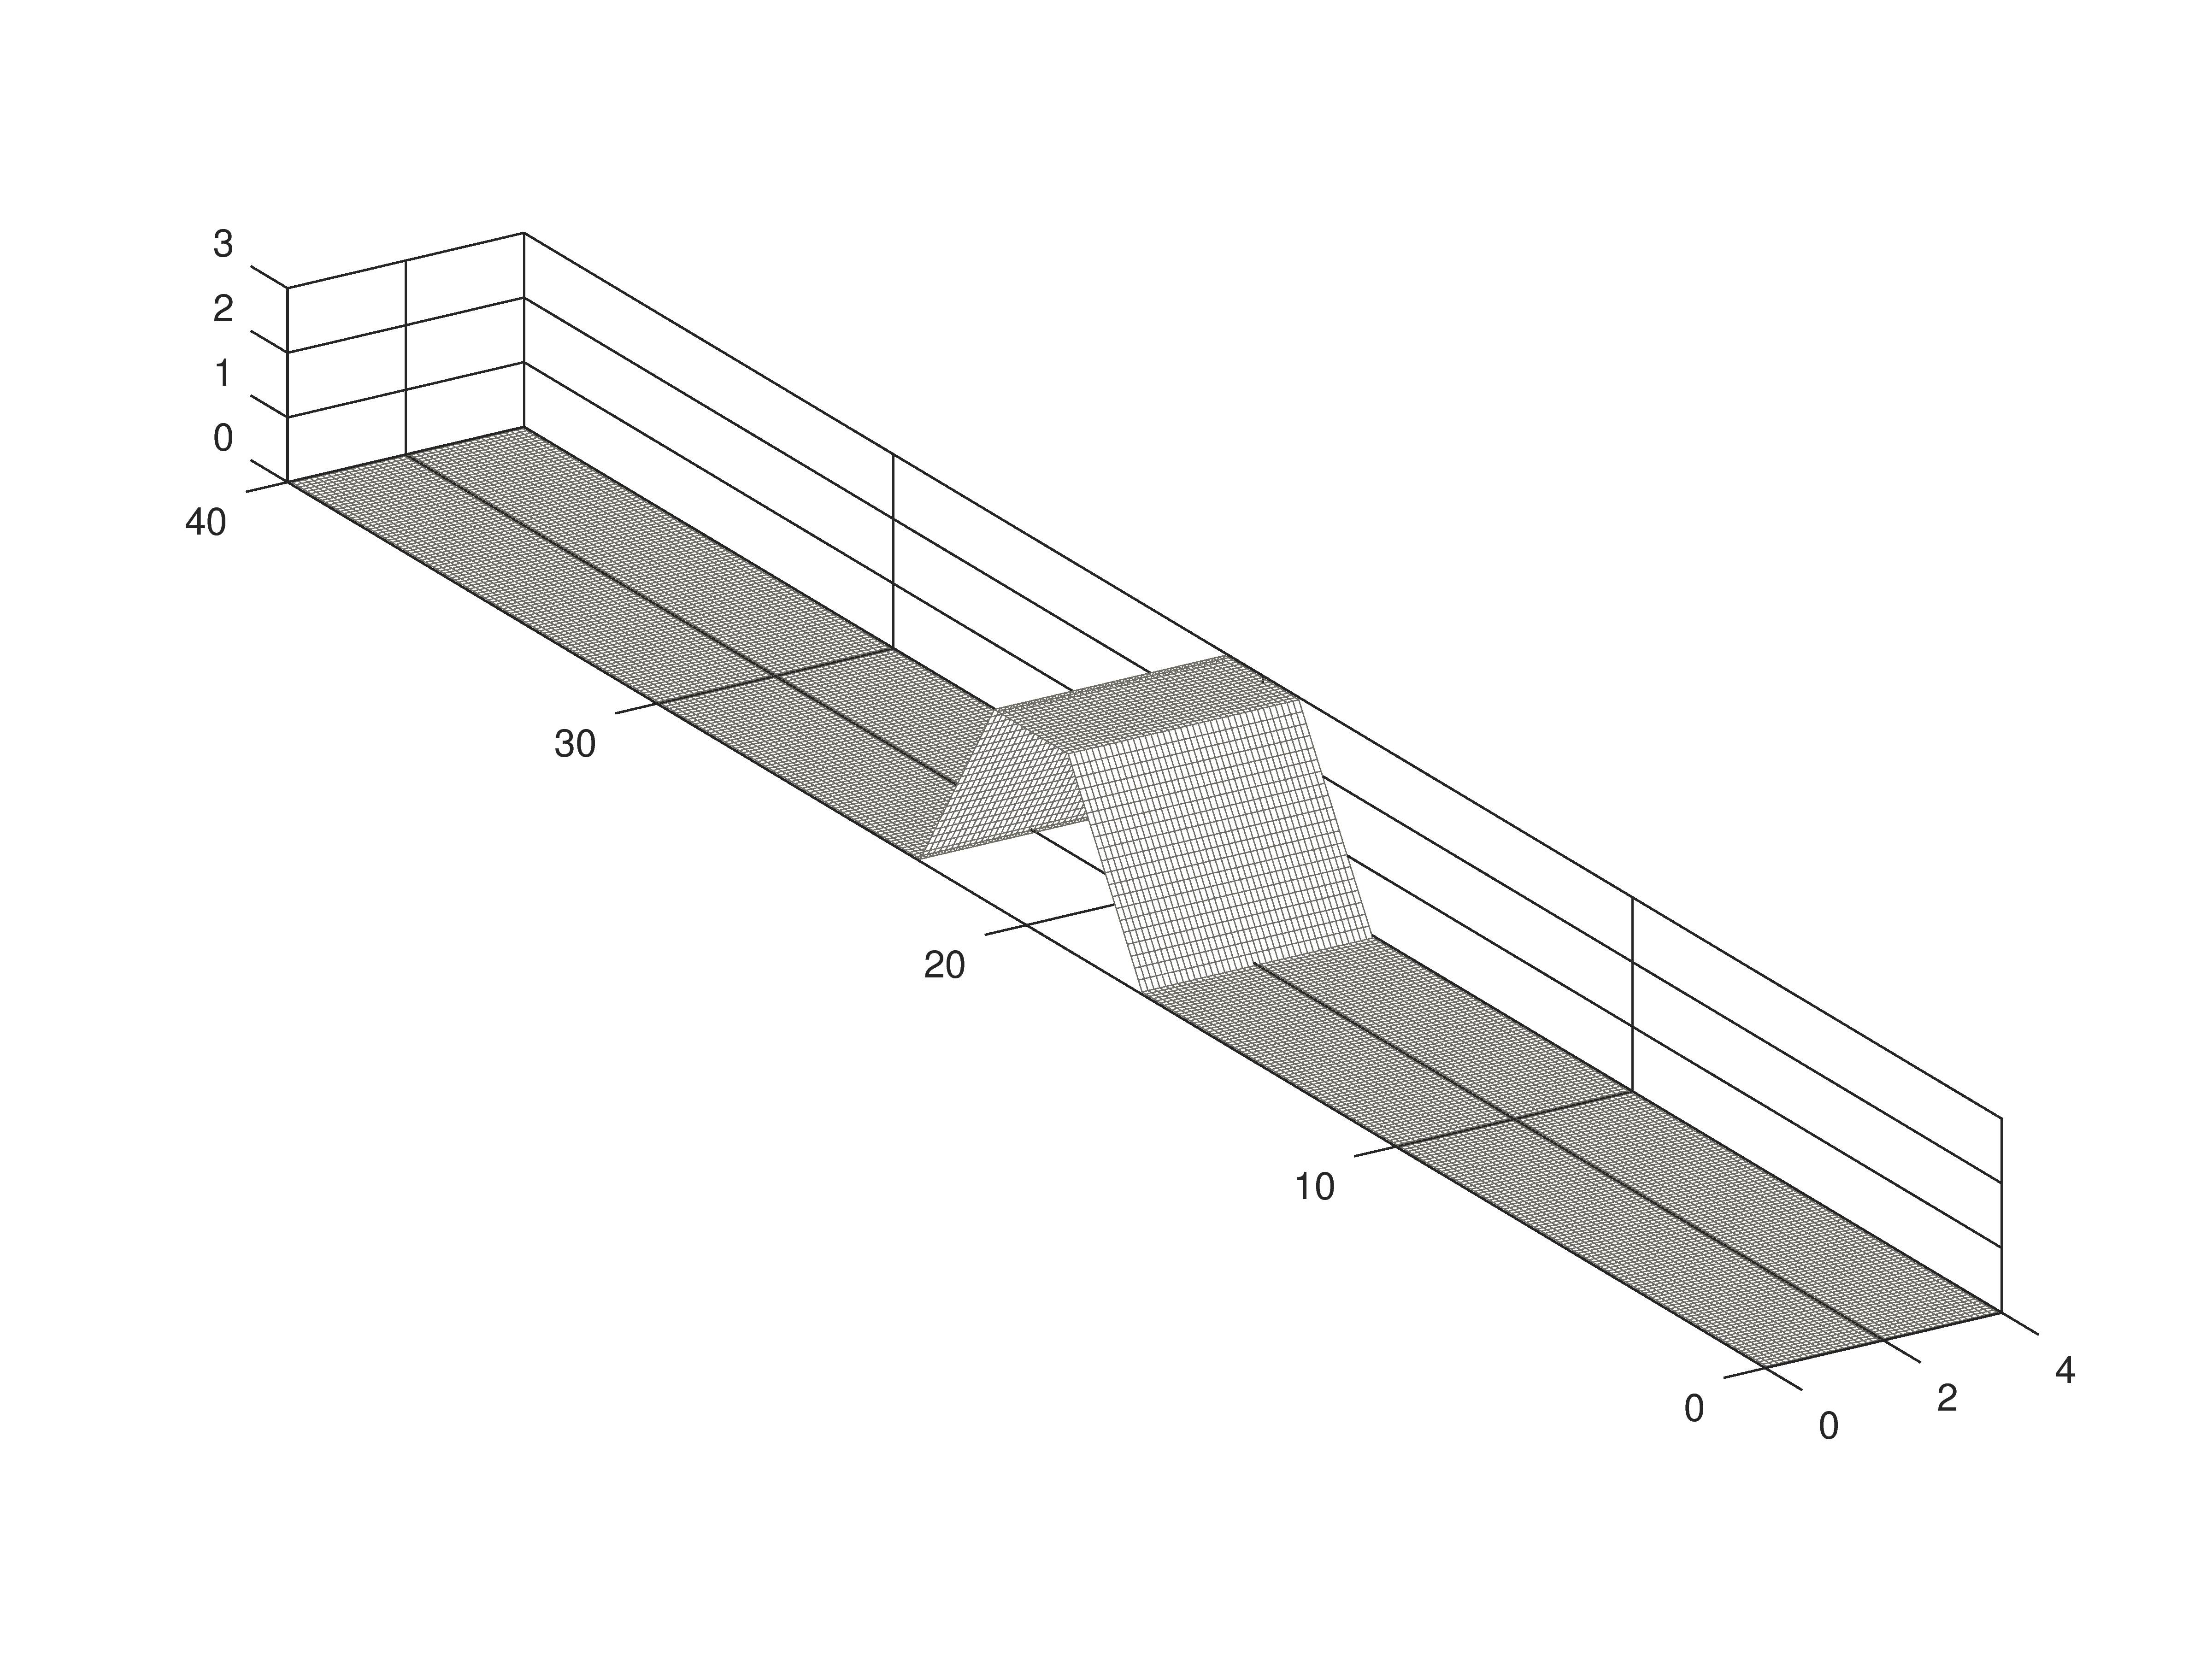
\includegraphics[width=0.8\textwidth]{Figures/channel.png}
  \caption{Channel topography and free surface of the water computed with \citetalias{delestre_fullswof:_2017} at $t = \SI{16}{\s}$. The simulation at this point has not reached the steady-state conditions yet. This is visible from the waves on the water surface downstream of the weir, indicating that the hydraulic jump has not stabilized yet.}
  \label{fig:channel}
\end{figure}
\seb{does it make sense to put this figure?}
\seb{change the caption of the figure!}


\begin{figure}[H]
  \centering
  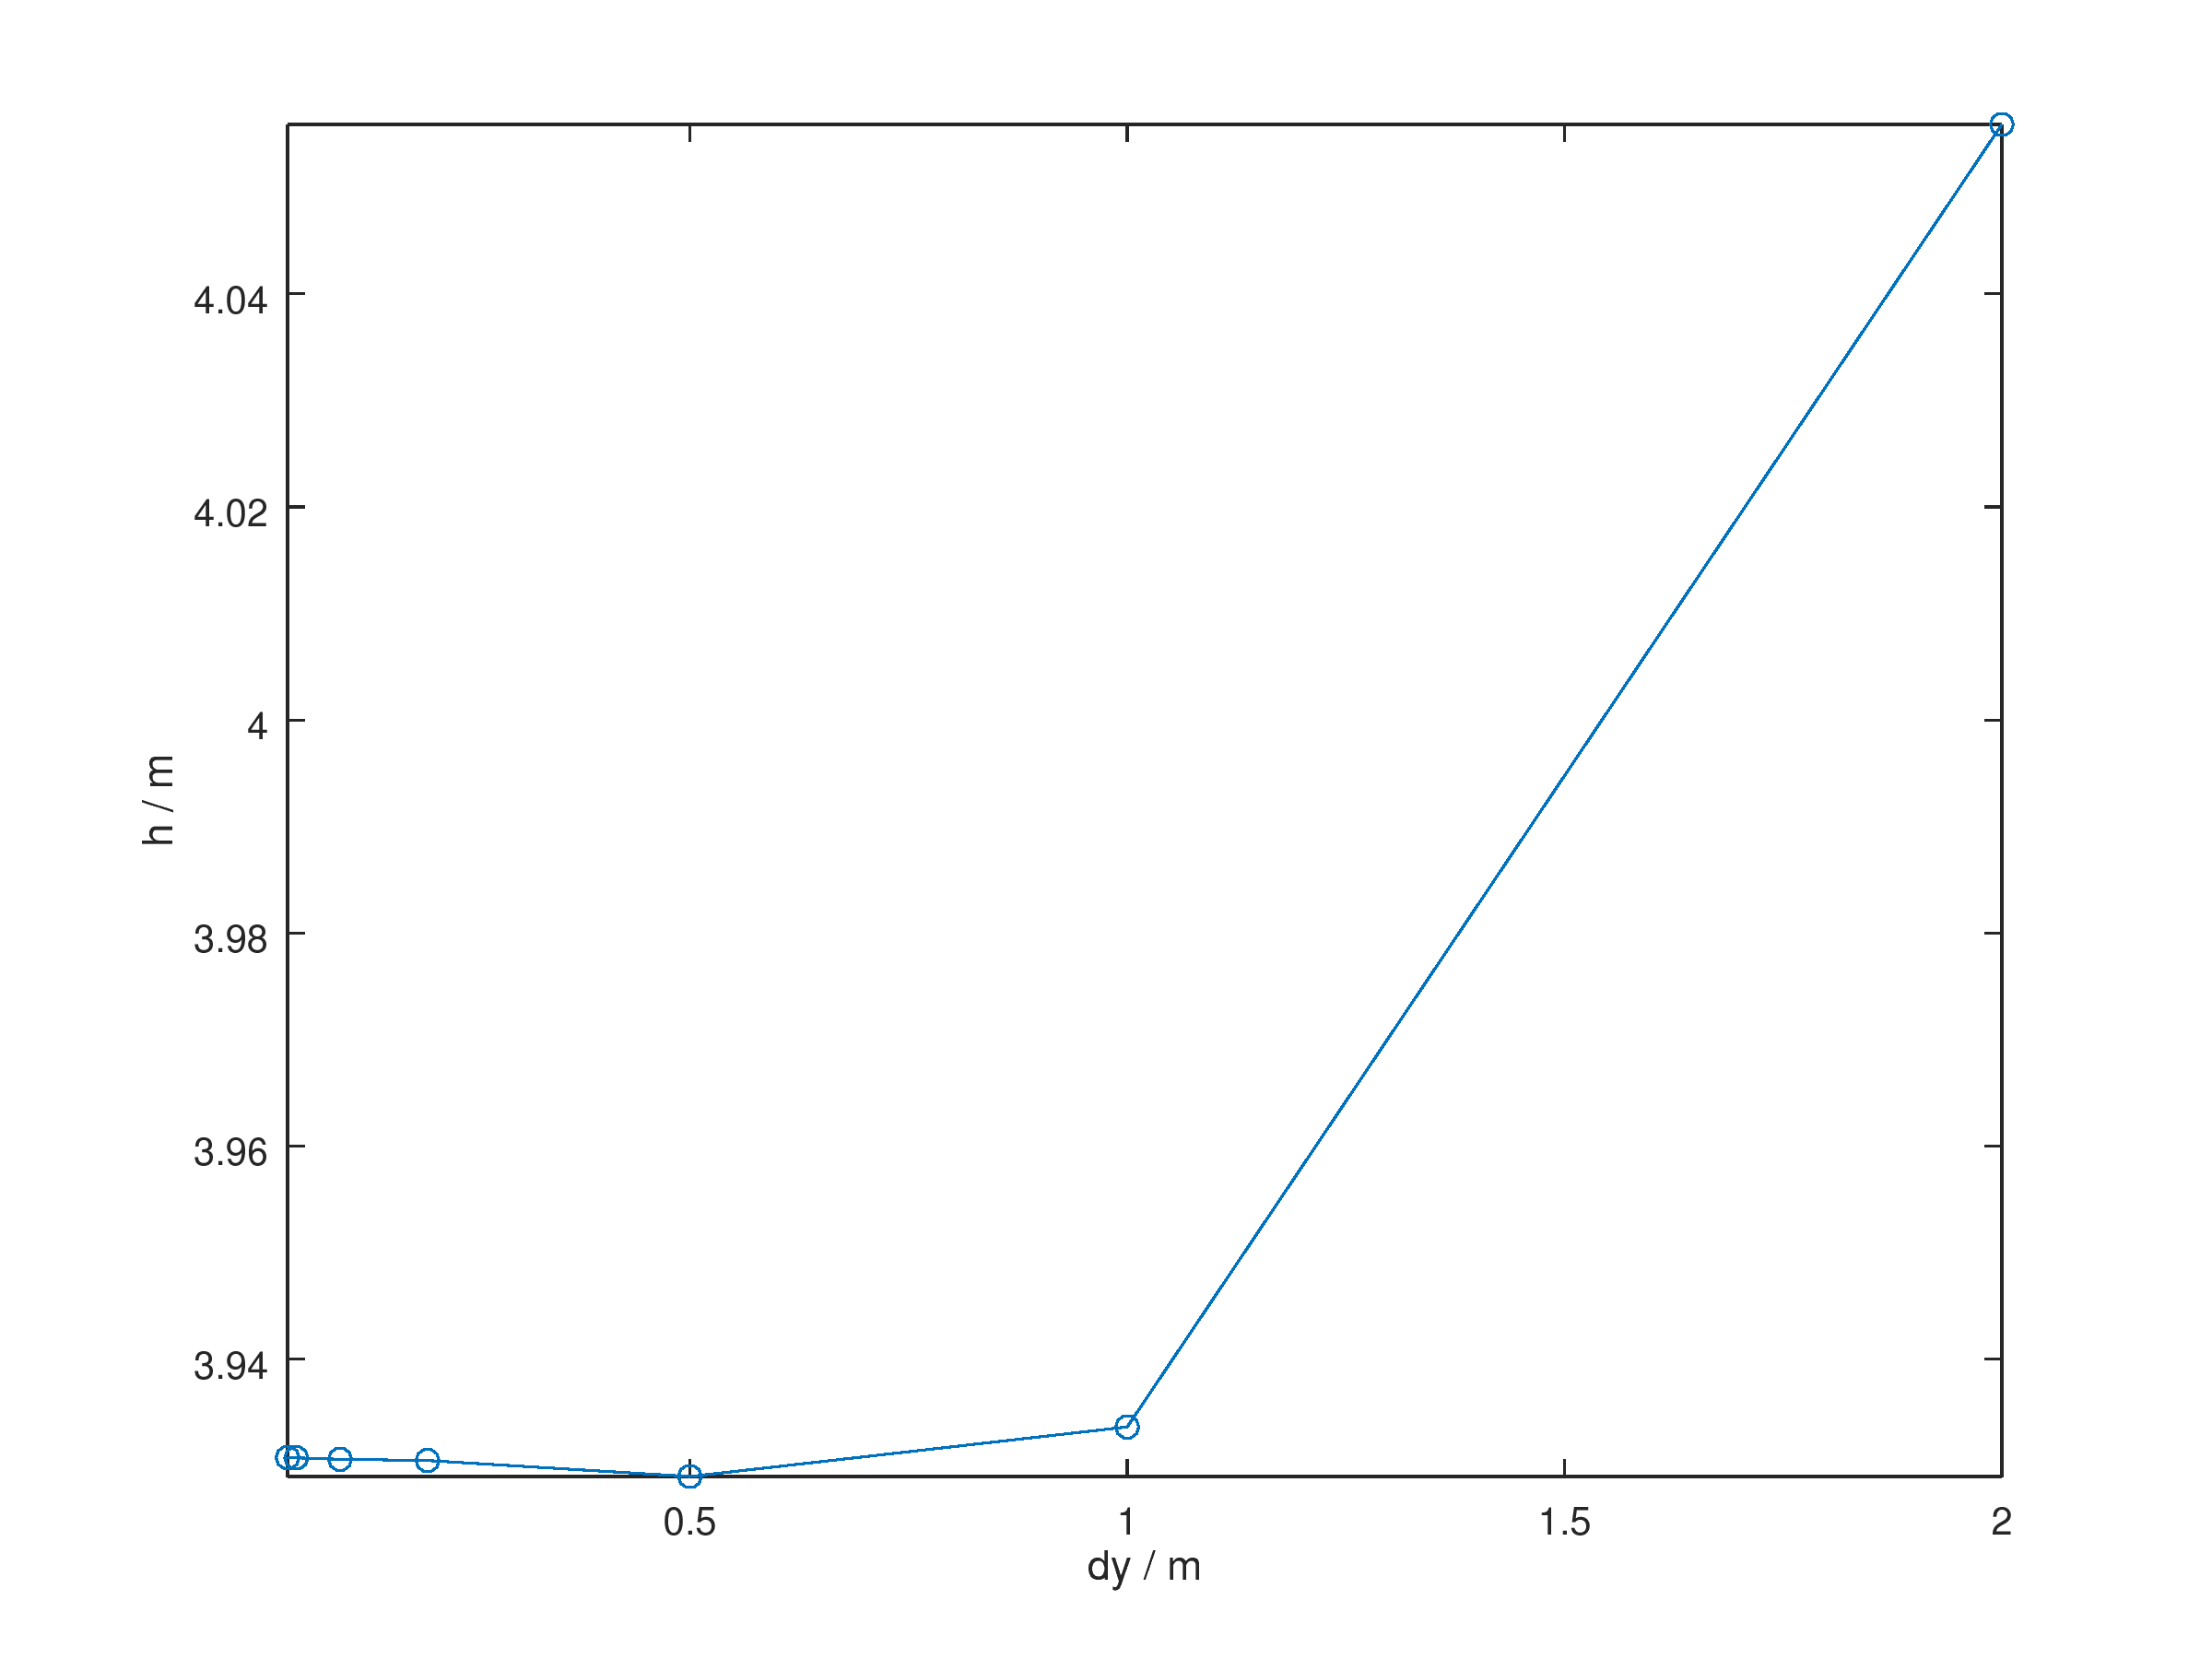
\includegraphics[width=0.7\textwidth]{Figures/convergence_center.png}
  \caption{Measured free surface height at the weir crest as a function of the grid resolution used.}
  \label{fig:convergence_center}
\end{figure}


\begin{table}[H]
  \centering
  \caption{Dataset used for computing the model error.}
  \label{tab:dataset_error}
  \begin{adjustbox}{max width=\textwidth}
    \begin{tabular}{lrrrrrrrrrrrrrr}
      \toprule
      $\bm{h_w}\,[\si{\m}]$             & 0.00 & 0.50 & 0.55 & 0.61 & 0.66 & 0.80 & 0.89 & 0.93 & 1.05 & 1.08 & 1.20 & 1.16 & 1.27 & 1.30\\
      $\bm{Q}\,[\si{\cubic\m\per\s}]$   & 0.00 & 2.16 & 2.58 & 2.99 & 3.40 & 4.64 & 5.46 & 5.88 & 7.11 & 7.53 & 8.76 & 8.35 & 9.59 & 10.00\\
      \bottomrule
    \end{tabular}}
  \end{adjustbox}
\end{table}


\begin{figure}[H]
  \centering
  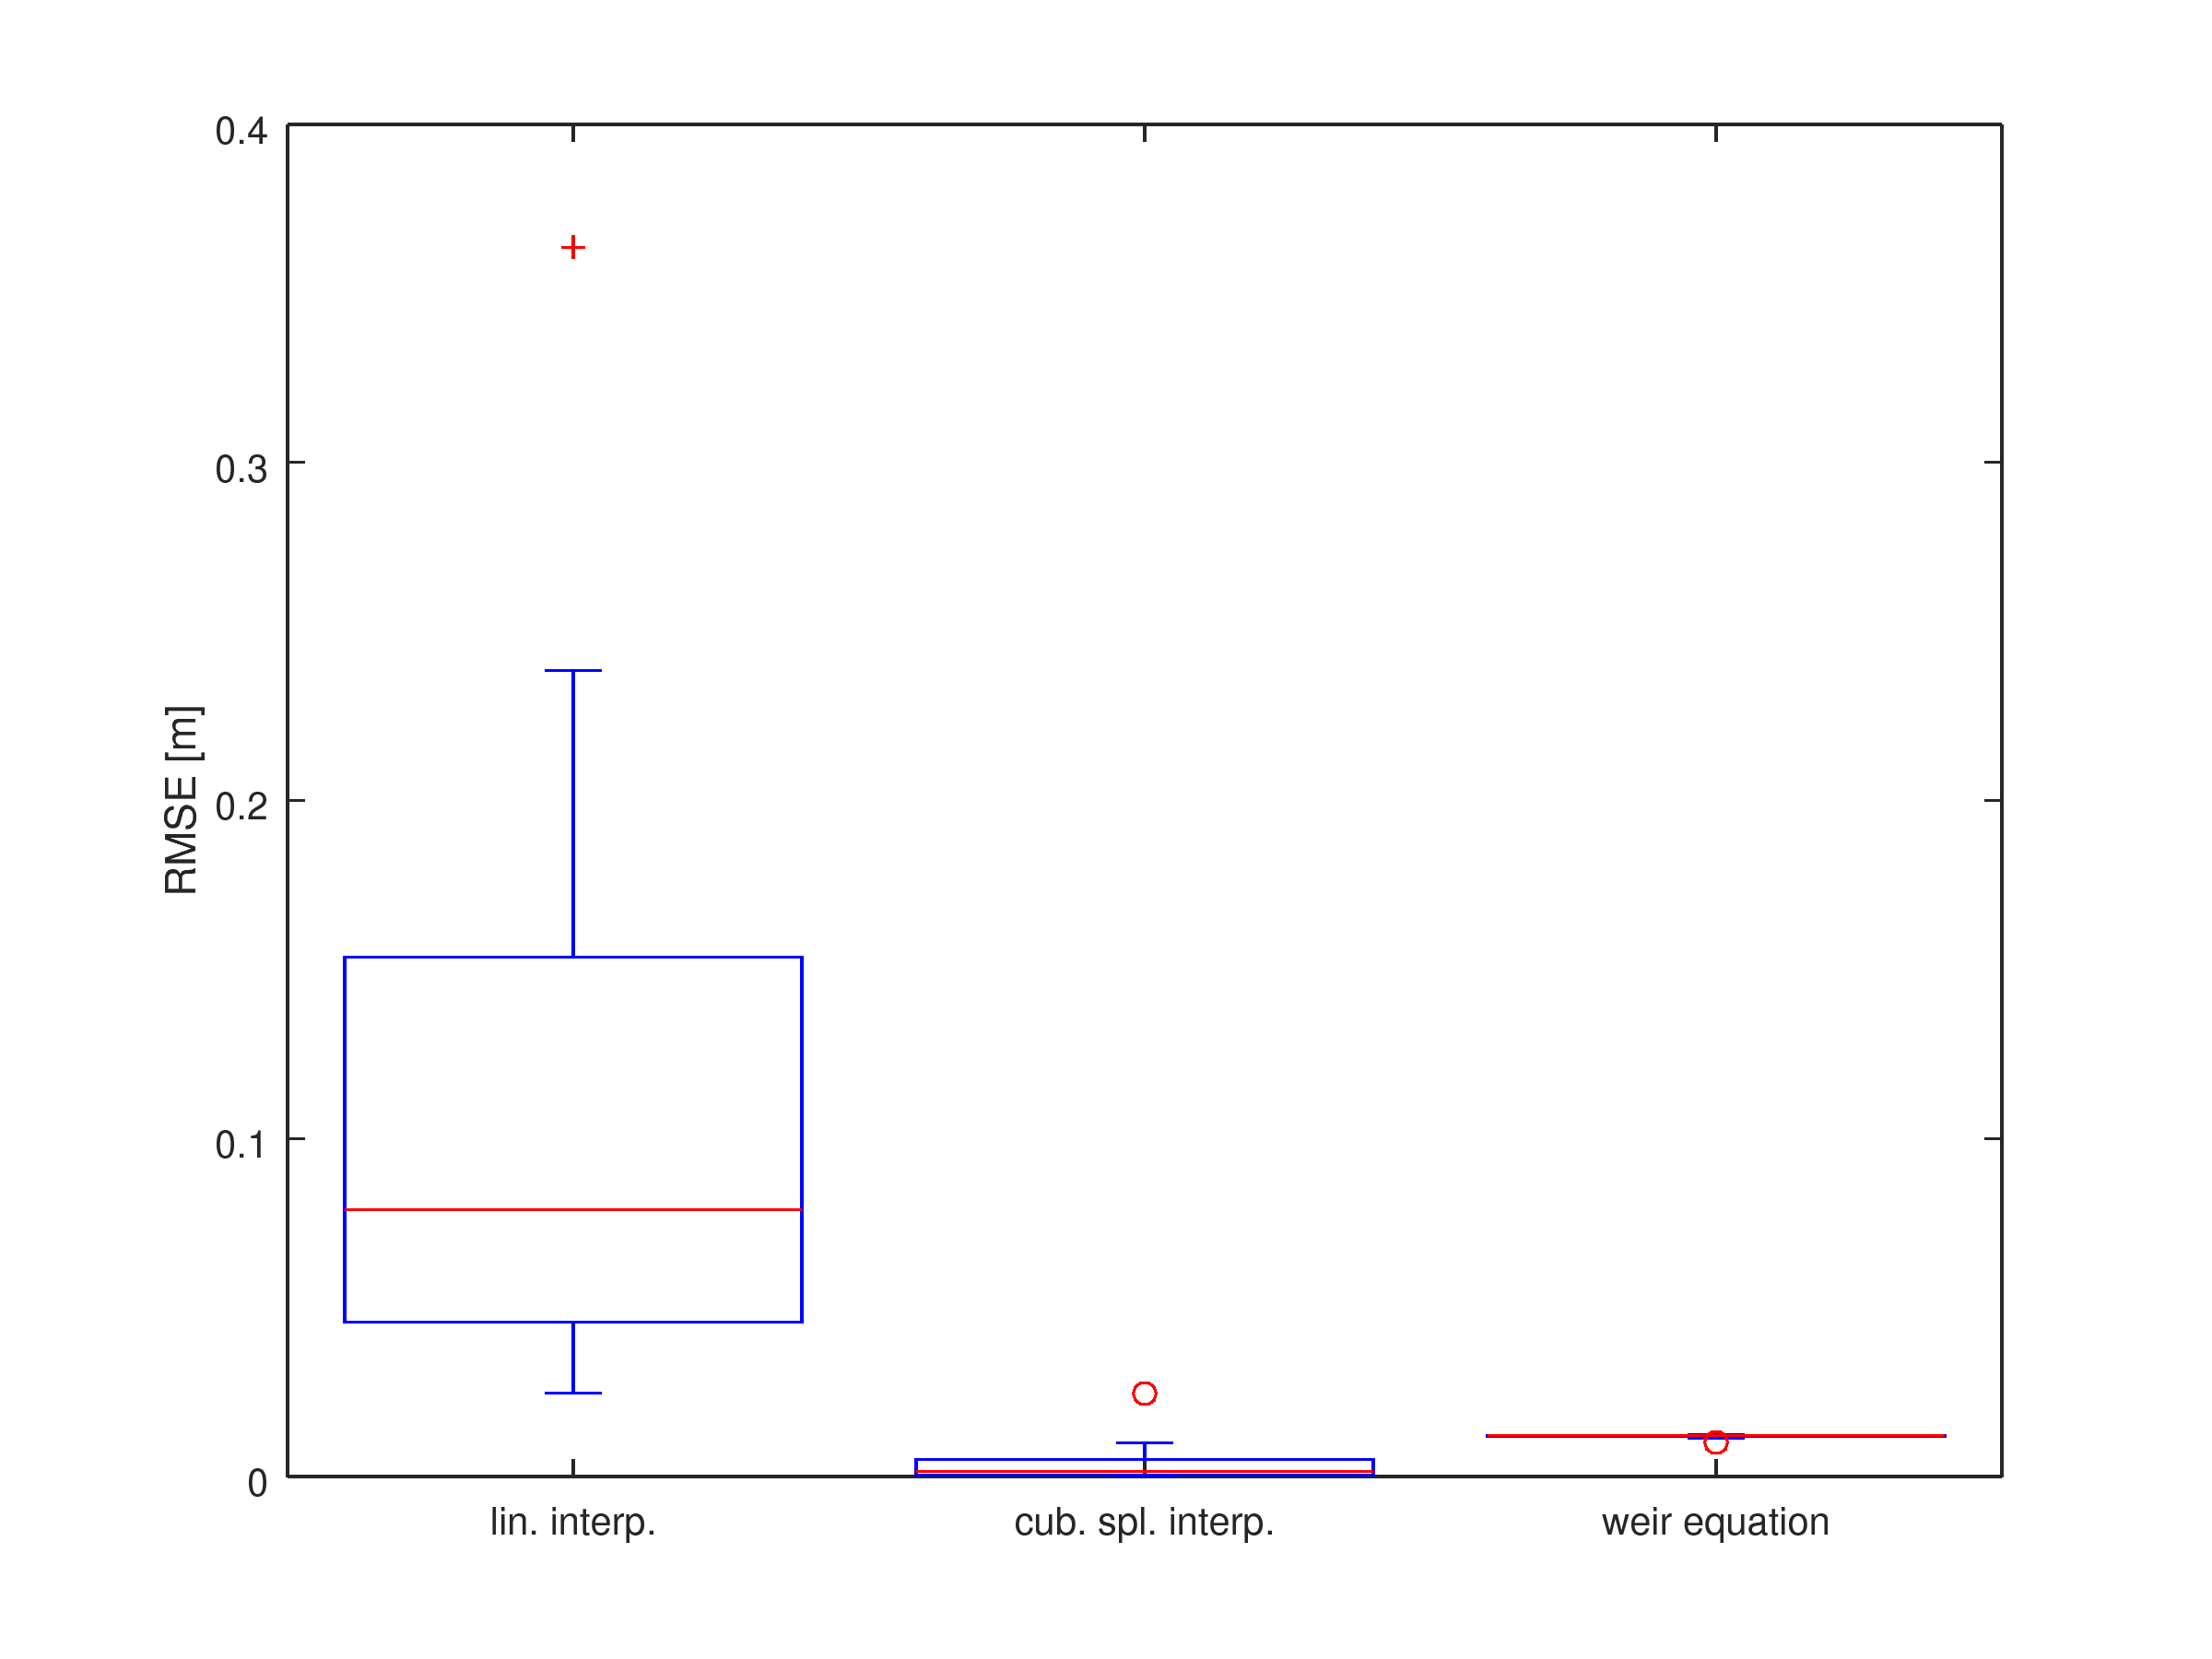
\includegraphics[width=0.7\textwidth]{Figures/boxplot_models.png}
  \caption{Box plot summarizing the performance of the three models by using $[\numrange{4}{13}]$ \# of points. The red line represent the median RMSE. The box is given by the \nth{1} and \nth{3} quartile. Whiskers are drawn at $1.5 \times IQR$. Points between $1.5 \times IQR$ and $3 \times IQR$ are marked with 'o', while '+' indicates points beyond this range \autocite{eaton_gnu_2016}.}
  \label{fig:boxplot_models}
\end{figure}

%===============================================================================
\section{Case study 2}
%===============================================================================
%-------------------------------------------------------------------------------
\subsection{Test dataset}\label{sec:test_dataset}
%-------------------------------------------------------------------------------
\inputminted[
  fontsize=\footnotesize,
  firstline=50,
  lastline=67,
  numbersep=2pt,
  gobble=0,
  frame=none,
  bgcolor=light-gray,
  framesep=10mm
]{octave}{code.m}

%-------------------------------------------------------------------------------
\subsection{Validation dataset}
%-------------------------------------------------------------------------------
\begin{table}[H]
  \centering
  \caption{Dataset used for the validation of the emulator.}
  \label{tab:validation_dataset}
  \begin{tabular}{ccccccc}
    \toprule
     & \textbf{1} & \textbf{2} & \textbf{3} & \textbf{4} & \textbf{5} & \textbf{6} \\
    \midrule
    $\bm{I}$ {\scriptsize[\si{\milli\meter\per\hour}]} & 15  & 20  & 22  & 25  & 25  & 35\\
    $\bm{\theta_i}$                                    & 0.9 & 0.2 & 0.5 & 0.8 & 0.4 & 0.8\\
    \bottomrule
  \end{tabular}
\end{table}

%-------------------------------------------------------------------------------
\subsection{Classification additional dataset}
%-------------------------------------------------------------------------------
\begin{table}[H]
  \centering
  \caption{Dataset used for the second, more accurate classification.}
  \label{tab:classification_dataset}
  \begin{tabular}{ccccccccc}
    \toprule
    $\bm{I}$ {\scriptsize[\si{\milli\meter\per\hour}]} & 11.2  & 12.0  & 13.5  & 14.7  & 15.4  & 15.8 & 16.3 & 17.0\\
    $\bm{\theta_i}$                                    & 0.95  & 0.80  & 0.60  & 0.45  & 0.35  & 0.3  & 0.20 & 0.05\\
    \bottomrule
  \end{tabular}
\end{table}


%-------------------------------------------------------------------------------
\subsection{"Rough" classifier}
%-------------------------------------------------------------------------------
\begin{figure}[H]
  \centering
  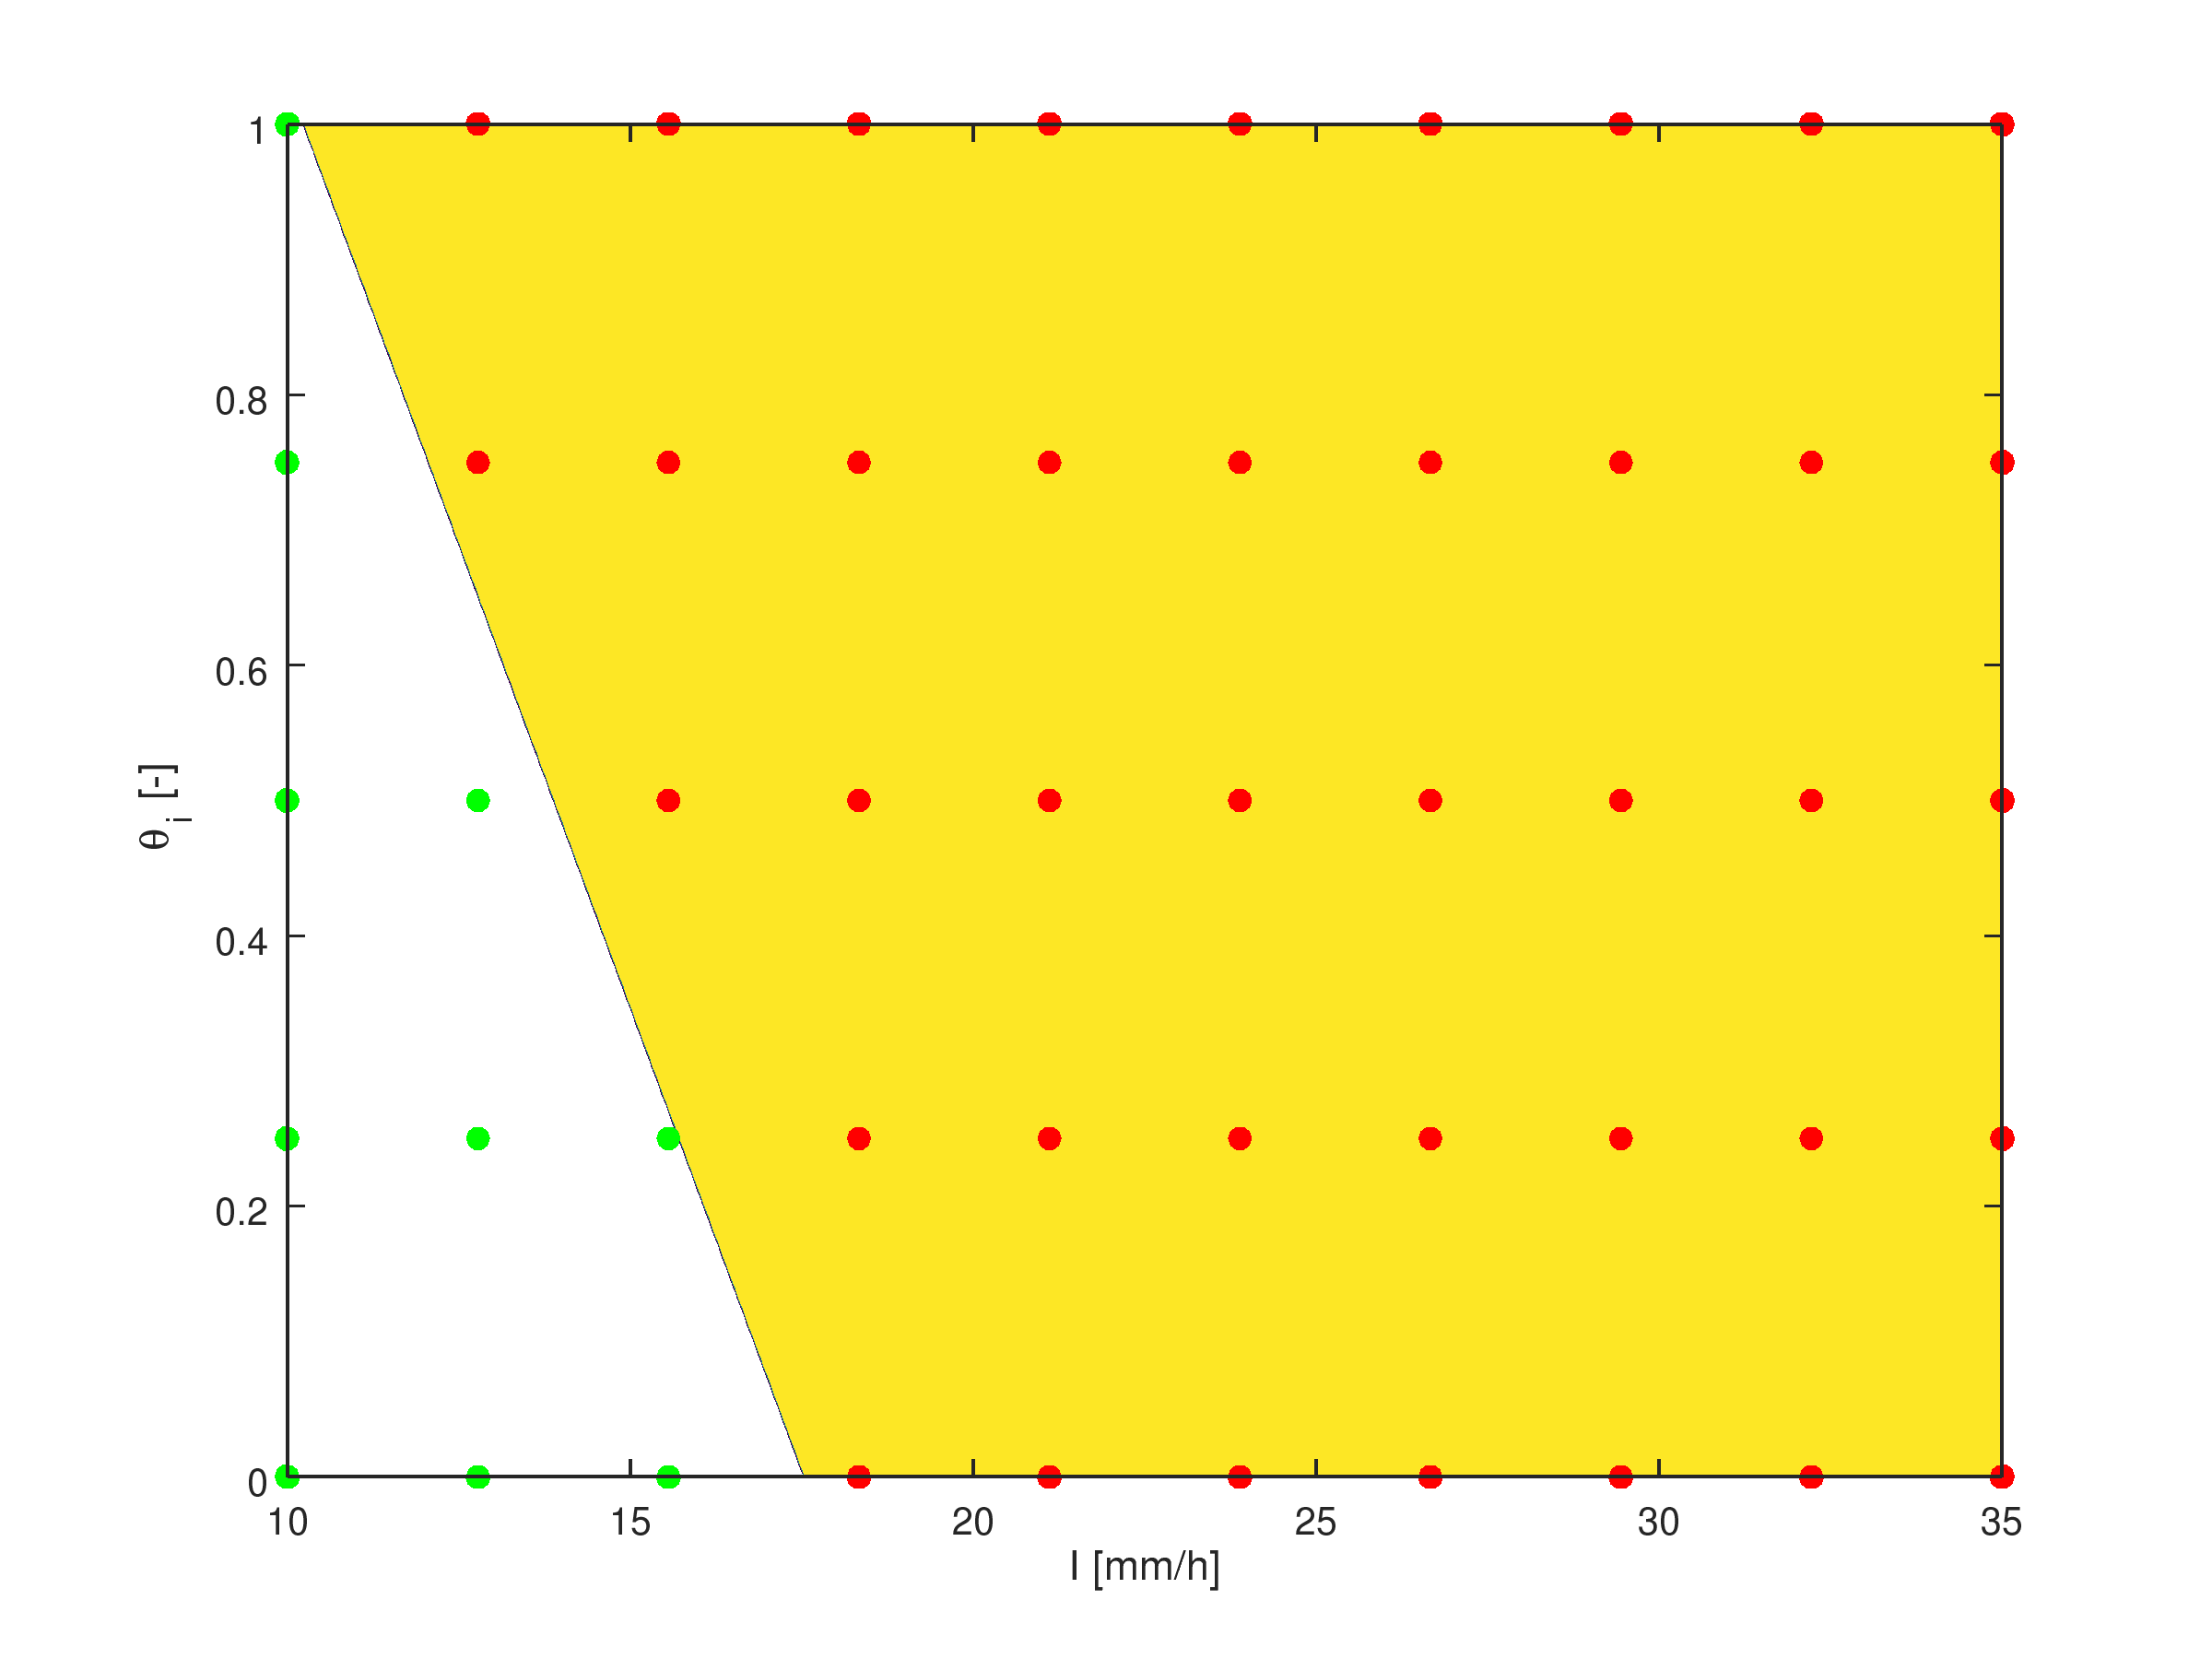
\includegraphics[width=0.7\textwidth]{Figures/classifier_trn.png}
  \caption{Linear separation of the training dataset with use of the "meanLinear" and "covConst" functions of the \citetalias{rasmussen_gaussian_2010} package. The linear classification works well on this dataset, but the shape of the boundary could be very different if more observations were present. An additional dataset with observations close to this boundary was created in order to refine the shape of the boundary.}
  \label{fig:classifier_rough}
\end{figure}

%-------------------------------------------------------------------------------
\subsection{Values of classifier's hyperparameters}\label{sec:classifier_hyperparameters}
%-------------------------------------------------------------------------------
\inputminted[
  fontsize=\footnotesize,
  firstline=115,
  lastline=132,
  numbersep=2pt,
  gobble=0,
  frame=none,
  bgcolor=light-gray,
  framesep=10mm
]{octave}{code.m}


%-------------------------------------------------------------------------------
\subsection{Values of emulator's hyperparameters}\label{sec:emulator_hyperparameters}
%-------------------------------------------------------------------------------
\inputminted[
  fontsize=\footnotesize,
  firstline=91,
  lastline=108,
  numbersep=2pt,
  gobble=0,
  frame=none,
  bgcolor=light-gray,
  framesep=10mm
]{octave}{code.m}


%-------------------------------------------------------------------------------
\subsection{Detailed validation performance}
%-------------------------------------------------------------------------------
\begin{table}[H]
  \centering
  \caption{Emulator performance on every validation point.}
  \label{tab:validation_performance}
  \begin{tabular}{lcccccc}
    \toprule
     & \textbf{1} & \textbf{2} & \textbf{3} & \textbf{4} & \textbf{5} & \textbf{6}\\
    \midrule
    \textbf{simulated} $\bm{t_!}\,[\si{\minute}]$     & 91.5 & 192.5 & 101.5 & 32.5 & 32.5 & 11.5\\
    \textbf{emulated}  $\bm{t_!}\,[\si{\minute}]$     & 86.2 & 198.0 & 95.5  & 32.4 & 34.0 & 11.0\\
    \textbf{error}     $\bm{\epsilon}\,[\si{\minute}]$ & 5.3  & -5.5  & 6.0   & 0.1  & -1.5 & 0.5\\
    \bottomrule
  \end{tabular}
\end{table}


%-------------------------------------------------------------------------------

\end{document}  
